% Options for packages loaded elsewhere
\PassOptionsToPackage{unicode}{hyperref}
\PassOptionsToPackage{hyphens}{url}
%
\documentclass[
]{book}
\usepackage{amsmath,amssymb}
\usepackage{lmodern}
\usepackage{iftex}
\ifPDFTeX
  \usepackage[T1]{fontenc}
  \usepackage[utf8]{inputenc}
  \usepackage{textcomp} % provide euro and other symbols
\else % if luatex or xetex
  \usepackage{unicode-math}
  \defaultfontfeatures{Scale=MatchLowercase}
  \defaultfontfeatures[\rmfamily]{Ligatures=TeX,Scale=1}
\fi
% Use upquote if available, for straight quotes in verbatim environments
\IfFileExists{upquote.sty}{\usepackage{upquote}}{}
\IfFileExists{microtype.sty}{% use microtype if available
  \usepackage[]{microtype}
  \UseMicrotypeSet[protrusion]{basicmath} % disable protrusion for tt fonts
}{}
\makeatletter
\@ifundefined{KOMAClassName}{% if non-KOMA class
  \IfFileExists{parskip.sty}{%
    \usepackage{parskip}
  }{% else
    \setlength{\parindent}{0pt}
    \setlength{\parskip}{6pt plus 2pt minus 1pt}}
}{% if KOMA class
  \KOMAoptions{parskip=half}}
\makeatother
\usepackage{xcolor}
\usepackage{color}
\usepackage{fancyvrb}
\newcommand{\VerbBar}{|}
\newcommand{\VERB}{\Verb[commandchars=\\\{\}]}
\DefineVerbatimEnvironment{Highlighting}{Verbatim}{commandchars=\\\{\}}
% Add ',fontsize=\small' for more characters per line
\usepackage{framed}
\definecolor{shadecolor}{RGB}{248,248,248}
\newenvironment{Shaded}{\begin{snugshade}}{\end{snugshade}}
\newcommand{\AlertTok}[1]{\textcolor[rgb]{0.94,0.16,0.16}{#1}}
\newcommand{\AnnotationTok}[1]{\textcolor[rgb]{0.56,0.35,0.01}{\textbf{\textit{#1}}}}
\newcommand{\AttributeTok}[1]{\textcolor[rgb]{0.77,0.63,0.00}{#1}}
\newcommand{\BaseNTok}[1]{\textcolor[rgb]{0.00,0.00,0.81}{#1}}
\newcommand{\BuiltInTok}[1]{#1}
\newcommand{\CharTok}[1]{\textcolor[rgb]{0.31,0.60,0.02}{#1}}
\newcommand{\CommentTok}[1]{\textcolor[rgb]{0.56,0.35,0.01}{\textit{#1}}}
\newcommand{\CommentVarTok}[1]{\textcolor[rgb]{0.56,0.35,0.01}{\textbf{\textit{#1}}}}
\newcommand{\ConstantTok}[1]{\textcolor[rgb]{0.00,0.00,0.00}{#1}}
\newcommand{\ControlFlowTok}[1]{\textcolor[rgb]{0.13,0.29,0.53}{\textbf{#1}}}
\newcommand{\DataTypeTok}[1]{\textcolor[rgb]{0.13,0.29,0.53}{#1}}
\newcommand{\DecValTok}[1]{\textcolor[rgb]{0.00,0.00,0.81}{#1}}
\newcommand{\DocumentationTok}[1]{\textcolor[rgb]{0.56,0.35,0.01}{\textbf{\textit{#1}}}}
\newcommand{\ErrorTok}[1]{\textcolor[rgb]{0.64,0.00,0.00}{\textbf{#1}}}
\newcommand{\ExtensionTok}[1]{#1}
\newcommand{\FloatTok}[1]{\textcolor[rgb]{0.00,0.00,0.81}{#1}}
\newcommand{\FunctionTok}[1]{\textcolor[rgb]{0.00,0.00,0.00}{#1}}
\newcommand{\ImportTok}[1]{#1}
\newcommand{\InformationTok}[1]{\textcolor[rgb]{0.56,0.35,0.01}{\textbf{\textit{#1}}}}
\newcommand{\KeywordTok}[1]{\textcolor[rgb]{0.13,0.29,0.53}{\textbf{#1}}}
\newcommand{\NormalTok}[1]{#1}
\newcommand{\OperatorTok}[1]{\textcolor[rgb]{0.81,0.36,0.00}{\textbf{#1}}}
\newcommand{\OtherTok}[1]{\textcolor[rgb]{0.56,0.35,0.01}{#1}}
\newcommand{\PreprocessorTok}[1]{\textcolor[rgb]{0.56,0.35,0.01}{\textit{#1}}}
\newcommand{\RegionMarkerTok}[1]{#1}
\newcommand{\SpecialCharTok}[1]{\textcolor[rgb]{0.00,0.00,0.00}{#1}}
\newcommand{\SpecialStringTok}[1]{\textcolor[rgb]{0.31,0.60,0.02}{#1}}
\newcommand{\StringTok}[1]{\textcolor[rgb]{0.31,0.60,0.02}{#1}}
\newcommand{\VariableTok}[1]{\textcolor[rgb]{0.00,0.00,0.00}{#1}}
\newcommand{\VerbatimStringTok}[1]{\textcolor[rgb]{0.31,0.60,0.02}{#1}}
\newcommand{\WarningTok}[1]{\textcolor[rgb]{0.56,0.35,0.01}{\textbf{\textit{#1}}}}
\usepackage{longtable,booktabs,array}
\usepackage{calc} % for calculating minipage widths
% Correct order of tables after \paragraph or \subparagraph
\usepackage{etoolbox}
\makeatletter
\patchcmd\longtable{\par}{\if@noskipsec\mbox{}\fi\par}{}{}
\makeatother
% Allow footnotes in longtable head/foot
\IfFileExists{footnotehyper.sty}{\usepackage{footnotehyper}}{\usepackage{footnote}}
\makesavenoteenv{longtable}
\usepackage{graphicx}
\makeatletter
\def\maxwidth{\ifdim\Gin@nat@width>\linewidth\linewidth\else\Gin@nat@width\fi}
\def\maxheight{\ifdim\Gin@nat@height>\textheight\textheight\else\Gin@nat@height\fi}
\makeatother
% Scale images if necessary, so that they will not overflow the page
% margins by default, and it is still possible to overwrite the defaults
% using explicit options in \includegraphics[width, height, ...]{}
\setkeys{Gin}{width=\maxwidth,height=\maxheight,keepaspectratio}
% Set default figure placement to htbp
\makeatletter
\def\fps@figure{htbp}
\makeatother
\setlength{\emergencystretch}{3em} % prevent overfull lines
\providecommand{\tightlist}{%
  \setlength{\itemsep}{0pt}\setlength{\parskip}{0pt}}
\setcounter{secnumdepth}{5}
\usepackage{booktabs}
\ifLuaTeX
  \usepackage{selnolig}  % disable illegal ligatures
\fi
\usepackage[]{natbib}
\bibliographystyle{plainnat}
\IfFileExists{bookmark.sty}{\usepackage{bookmark}}{\usepackage{hyperref}}
\IfFileExists{xurl.sty}{\usepackage{xurl}}{} % add URL line breaks if available
\urlstyle{same} % disable monospaced font for URLs
\hypersetup{
  pdftitle={Leaflet book},
  pdfauthor={Samuel Gachuhi Ngugi},
  hidelinks,
  pdfcreator={LaTeX via pandoc}}

\title{Leaflet book}
\author{Samuel Gachuhi Ngugi}
\date{2023-06-21}

\begin{document}
\maketitle

{
\setcounter{tocdepth}{1}
\tableofcontents
}
\hypertarget{about}{%
\chapter*{About}\label{about}}
\addcontentsline{toc}{chapter}{About}

This is a \emph{sample} book written in \textbf{Markdown}. You can use anything that Pandoc's Markdown supports; for example, a math equation \(a^2 + b^2 = c^2\).

\hypertarget{usage}{%
\section*{Usage}\label{usage}}
\addcontentsline{toc}{section}{Usage}

Each \textbf{bookdown} chapter is an .Rmd file, and each .Rmd file can contain one (and only one) chapter. A chapter \emph{must} start with a first-level heading: \texttt{\#\ A\ good\ chapter}, and can contain one (and only one) first-level heading.

Use second-level and higher headings within chapters like: \texttt{\#\#\ A\ short\ section} or \texttt{\#\#\#\ An\ even\ shorter\ section}.

The \texttt{index.Rmd} file is required, and is also your first book chapter. It will be the homepage when you render the book.

\hypertarget{render-book}{%
\section*{Render book}\label{render-book}}
\addcontentsline{toc}{section}{Render book}

You can render the HTML version of this example book without changing anything:

\begin{enumerate}
\def\labelenumi{\arabic{enumi}.}
\item
  Find the \textbf{Build} pane in the RStudio IDE, and
\item
  Click on \textbf{Build Book}, then select your output format, or select ``All formats'' if you'd like to use multiple formats from the same book source files.
\end{enumerate}

Or build the book from the R console:

\begin{Shaded}
\begin{Highlighting}[]
\NormalTok{bookdown}\SpecialCharTok{::}\FunctionTok{render\_book}\NormalTok{()}
\end{Highlighting}
\end{Shaded}

To render this example to PDF as a \texttt{bookdown::pdf\_book}, you'll need to install XeLaTeX. You are recommended to install TinyTeX (which includes XeLaTeX): \url{https://yihui.org/tinytex/}.

\hypertarget{preview-book}{%
\section*{Preview book}\label{preview-book}}
\addcontentsline{toc}{section}{Preview book}

As you work, you may start a local server to live preview this HTML book. This preview will update as you edit the book when you save individual .Rmd files. You can start the server in a work session by using the RStudio add-in ``Preview book'', or from the R console:

\begin{Shaded}
\begin{Highlighting}[]
\NormalTok{bookdown}\SpecialCharTok{::}\FunctionTok{serve\_book}\NormalTok{()}
\end{Highlighting}
\end{Shaded}

\hypertarget{introduction}{%
\chapter{Introduction}\label{introduction}}

\hypertarget{what-is-leaflet}{%
\section{What is Leaflet?}\label{what-is-leaflet}}

Something to do with leaves? Of course not.Leaflet, when bare scrapped to its most basic definition, is simply an open source JavaScript library for interactive maps. It was developed in 2011 by Volodymyr Agafonkin, a Ukrainain with a mathematical background.

\hypertarget{how-does-it-work}{%
\section{How does it work?}\label{how-does-it-work}}

Leaflet can work if every line of code is inside a \texttt{html} document, so long as the code appears under the \texttt{\textless{}script\textgreater{}} tag. However, for a neat work, especially working with complex maps, it is recommended you separate the \texttt{html} file from its other components of \texttt{main.js} and \texttt{style.css} files.

``HTML we know, but what are \texttt{main.js} and \texttt{style.css} files?'', you may ask.

Well, beginning with \texttt{html}, which stands for \textbf{Hypertext Markup Language}, it is the language that is \href{https://www.tutorialspoint.com/html/index.htm}{used in creating webpages}. It is actually the standard of making static webmaps. I am yet to come across any webpage that is made up of everything apart from HTML. If you want to have a view of what HTML looks like, just right click any webpage and click \emph{Inspect} in Google Chrome and Firefox. A toolbar will appear at the bottom or side of the webpage, depending on your settings.

\begin{Shaded}
\begin{Highlighting}[]
\NormalTok{knitr}\SpecialCharTok{::}\FunctionTok{include\_graphics}\NormalTok{(}\FunctionTok{rep}\NormalTok{(}\StringTok{"D:/gachuhi/my{-}leaflet/images/inspect.jpg"}\NormalTok{))}
\end{Highlighting}
\end{Shaded}

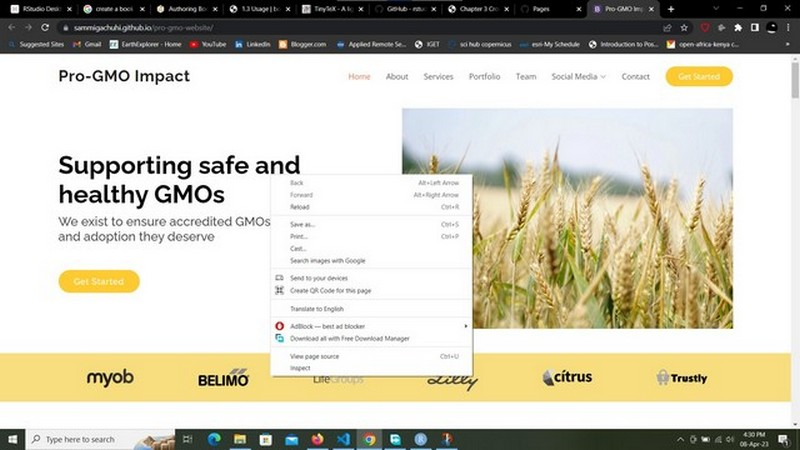
\includegraphics[width=11.11in]{../images/inspect}

Scroll over to the \textbf{Element} tab and you will have something that looks like this:

\begin{Shaded}
\begin{Highlighting}[]
\NormalTok{knitr}\SpecialCharTok{::}\FunctionTok{include\_graphics}\NormalTok{(}\FunctionTok{rep}\NormalTok{(}\StringTok{"D:/gachuhi/my{-}leaflet/images/elements.jpg"}\NormalTok{))}
\end{Highlighting}
\end{Shaded}

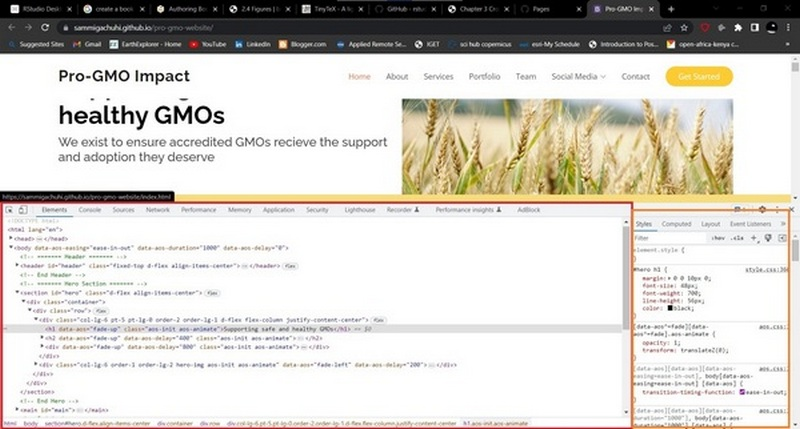
\includegraphics[width=11.11in]{../images/elements}

The part encircled in red is the \texttt{html} that makes up the webpage for the \href{https://sammigachuhi.github.io/pro-gmo-website/}{ProGMO website} in this case.

So, I am a GIS specialist, I want to learn how to make a html website so as to use leaflet and its functionalities. Whereas this document does not provide an indepth view of all the ins and outs of a html document, html websites are made up of elements known as \texttt{tags}. Tags, normally indicated by angle brackets (\texttt{\textless{}\textgreater{}}) are what introduce any form of content into a webpage, be it a paragraph \texttt{(\textless{}p\textgreater{})}, an image \texttt{(\textless{}img\textgreater{})}, video \texttt{(\textless{}video\textgreater{})} and even an entire section (\texttt{\textless{}div\textgreater{}}, \texttt{\textless{}section\textgreater{}}, \texttt{\textless{}article\textgreater{}}). With this basic introduction, let's create a basic html page.

To create a html element along with many other programming files, such as \texttt{.js} and \texttt{.css} which we shall see later, we use a text editor. A good example of a text editor is VS code or Pycharm. Check their websites on their installation methods for your personal computer. For creating html and working with \texttt{.js} documents later, we shall use VS Code unless otherwise stated.

Here is a basic html webpage.

\begin{verbatim}
<!DOCTYPE html>
<html lang="en">
    <head>
        <title>A basic html webpage</title>
        <meta charset="utf-8">
        <link rel="stylesheet" href="style.css">
    </head>
    <body>
        <div id="division-1">
            <p>Hello, World!</p>
        </div>
        <script src="main.js">

        </script>

    </body>
</html>
\end{verbatim}

Let's go through the above tags one by one.

\begin{enumerate}
\def\labelenumi{\arabic{enumi}.}
\item
  \texttt{\textless{}!DOCTYPE\ html\textgreater{}} - It is an ``information'' to the browser about what document type to expect.
\item
  \texttt{\textless{}html\ lang="en"\textgreater{}} - It is the container for all other HTML elements (except for the \texttt{\textless{}!DOCTYPE\textgreater{}} tag). The \texttt{lang} attribute is used to assist web engines know which language the website uses.
\item
  \texttt{\textless{}head\textgreater{}} - It is not displayed on the webpage as other tags, but contains the metadata of the webpage.
\item
  \texttt{\textless{}title\textgreater{}} - Can you guess? You had it right. Defines the title of the document. In our case, if you open the webpage assuming you created it in VS Code, the webpage shall be titled \emph{A basic html webpage} at the tab of your web-browser.
\item
  \texttt{\textless{}meta\ charset="utf-8"\textgreater{}} - This is one of the metadata hosted by the \texttt{\textless{}head\textgreater{}} tag. We had mentioned earlier that the \texttt{\textless{}head\textgreater{}} contains the metadata of the webpage. Now here we would like to add that the \texttt{\textless{}meta\textgreater{}} tag found \emph{within} the \texttt{\textless{}head\textgreater{}} is what \emph{defines} the metadata. You can think of it as \textbf{README} text file that comes with any software you download. The \texttt{\textless{}meta\textgreater{}} tag in our case defines the encoding of our HTML5 document with the attribute \texttt{charset="utf-8"}. Don't think about this too much. HTML5 documents have \texttt{utf-8} as their encoding. You can try to look up what encoding is but it's not useful for this tutorial!
\item
  \texttt{\textless{}link\textgreater{}} - Defines the relationship between a document and an external resource. It has various attributes but \texttt{rel} and \texttt{href} have been used. The former specifies the relationship between the current document and the linked document/resource. The \texttt{rel} here references the \texttt{styles.css} file as the style sheet for our html. That is, the styles for our html are found in the \texttt{styles.css} file. \texttt{href} on the other hand points the html document to the path of the stylesheet --the \texttt{styles.css} file.
\item
  \texttt{\textless{}body\textgreater{}} - This is the crux of your webpage. If nothing is within the \texttt{\textless{}body\textgreater{}} tags, your webpage will be as empty as a blank sheet of paper. This tag is the home for all the other contents of the webpage such as headings, paragraphs, images, tables etc.
\item
  \texttt{\textless{}div\textgreater{}} - This is a special element that lets you group similar sets of content together on a web page. You can use it as a generic container for associating similar content. In the above html script, we have included an \texttt{\textless{}id\textgreater{}} attribute that is in other words, a unique identifier for this section of the webpage. \texttt{\textless{}id\textgreater{}s} are useful if you want to customize the appearance of a certain part of the webpage. \texttt{\textless{}class\textgreater{}}es behave in a similar way, but the difference between \texttt{\textless{}id\textgreater{}} and \texttt{\textless{}class\textgreater{}} is that \texttt{\textless{}id\textgreater{}} has to be unique, while \texttt{\textless{}class\textgreater{}}es can be used more than once.
\end{enumerate}

9.\texttt{\textless{}script\textgreater{}} - It is used to embed executable code or data. In most cases it refers to JavaScript, which enhances interactivity.

If you may have noticed above, most HTML tags end with \texttt{\textless{}/name-of-tag\textgreater{}}. With a few exceptions such as \texttt{\textless{}img\textgreater{}}, almost all HTML tags end this way.

\hypertarget{javascript}{%
\section{JavaScript}\label{javascript}}

JavaScript, shortened to \texttt{.js} is the language of the web. It introduces interactivity to HTML files. Without it our HTML files would just remain static. Have you ever clicked a link or a shiny button on a website and some visual or menu popped up? JavaScript was the engine behind all that. Think of \texttt{.js} as the life of the party while HTML is just the setting. Without \texttt{.js} creating webmaps would not be possible since adding JavaScript code to a html file using \texttt{\textless{}script\textgreater{}} is what makes the map appear on any website!

\hypertarget{css-files}{%
\section{CSS files}\label{css-files}}

CSS stands for \emph{Cascading Style Sheet}. The CSS defines how your HTML is to appear, such as color and size of text, background color of the HTML as well as the structure of your HTML page.

CSS is quite a huge field despite being simple. However, the html elements of a webpage are accompanied by a curly bracket containing the specified properties and values.

\begin{itemize}
\item
  Properties: These are human-readable identifiers that indicate which stylistic features you want to modify. For example, font-size, width, background-color.
\item
  Values: Each property is assigned a value. This value indicates how to style the property.
\end{itemize}

Using the example of our ProGMO website, this is how we would specify the font and color of the \texttt{\textless{}body\textgreater{}} element of our webpage. In some cases, the property values in CSS elements can be more than one, as in \texttt{font-family} below.

\begin{verbatim}
body {
  font-family: "Open Sans", sans-serif;
  color: #444444;
}
\end{verbatim}

The \texttt{body} in the CSS file is known as the selector. Selectors in CSS are what tags are in HTML files. However, selectors can be more specific, such as specifying the exact \texttt{\textless{}div\textgreater{}} that should be displayed in a particular way. Using our html file example, if there were other \texttt{\textless{}div\textgreater{}}s apart from the \texttt{\textless{}div\ id="division-1"\textgreater{}} above, we would specify our first one in a CSS document like so:

\begin{verbatim}
#division-1 {
  font-family: "Open Sans", sans-serif;
  color: #343a40;
}
\end{verbatim}

We would specify other property values for our \texttt{\textless{}div\textgreater{}}s by their names following a \texttt{\#} like so. Suppose there was a \texttt{\textless{}div\ id="division-2"\textgreater{}} somewhere in the HTML we could define some properties specific to it in the manner below:

\begin{verbatim}
#division-2 {
  font-family: helvetica;
  color: #000000;
}
\end{verbatim}

For \texttt{\textless{}classes\textgreater{}} and they can be several, we select each particular class using the convention:

\begin{verbatim}
.class_name {
property: value
prperty2: value2}
\end{verbatim}

You can view the style of a particular HTML element using the styles tab found in the inspect console. It is shown in yellow bounds for a chrome webpage. Firefox should have a similar one.

\begin{Shaded}
\begin{Highlighting}[]
\NormalTok{knitr}\SpecialCharTok{::}\FunctionTok{include\_graphics}\NormalTok{(}\FunctionTok{rep}\NormalTok{(}\StringTok{"D:/gachuhi/my{-}leaflet/images/elements2.jpg"}\NormalTok{))}
\end{Highlighting}
\end{Shaded}

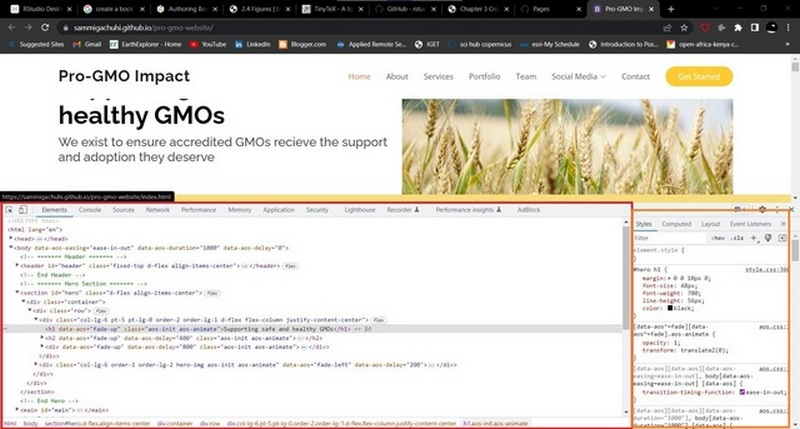
\includegraphics[width=11.11in]{../images/elements2}

The \href{https://developer.mozilla.org/en-US/docs/Learn/CSS/First_steps/How_CSS_is_structured}{MDN website} provides a lot of information on HTML and CSS.

\hypertarget{summary}{%
\section{Summary}\label{summary}}

This chapter was an introduction to Hyper Text Markup Language (HTML), JavaScript and Cascading Style Sheets (CSS) languages. You learnt the following:

\begin{itemize}
\item
  You can work with leaflet in either a html or JavaScript file. In html,
  the JavaScript code must appear under the \texttt{\textless{}script\textgreater{}} tag.
\item
  HTML files are made up of elements called tags. Tags are features that introduce any form of content into a webpage.
\item
  JavaScript is the main language of the web. It is the language responsible for the interactivity in most websites.
\item
  CSS stands for Cascading Style Sheet (CSS). CSS defines how your HTML is to appear, such as color and size of text, background color and even the structure of your HTML page.
\end{itemize}

\hypertarget{first-leaflet-map}{%
\chapter{First Leaflet Map}\label{first-leaflet-map}}

\hypertarget{setting-the-superstructure}{%
\section{Setting the superstructure}\label{setting-the-superstructure}}

We had earlier mentioned that Javascript, otherwise shortened to JS is the life of the party when it comes to webpages. In other words, it makes your web pages interactive. It's like the additional component that makes your HTML pages move from static to responsive.

Creating a leaflet map is not like creating any other HTML web page. You have to set up the leaflet essentials in your HTML page first. To begin with, create a new html document called \texttt{map.html}. This will be the html document that will act as the structure which will house our webpage to be created using JS. Using VS Code, create \texttt{map.html} and paste, or preferably, type the following code.

\begin{verbatim}
<!DOCTYPE html>
<html lang="en">
    <head>
        <title>Leaflet Maps</title>
        <meta charset="utf-8">
        <link rel="stylesheet" href="styles.css">
        <link rel="stylesheet" href="https://unpkg.com/leaflet@1.9.3/dist/leaflet.css"
     integrity="sha256-kLaT2GOSpHechhsozzB+flnD+zUyjE2LlfWPgU04xyI="
     crossorigin=""/>
        <script src="https://unpkg.com/leaflet@1.9.3/dist/leaflet.js"
        integrity="sha256-WBkoXOwTeyKclOHuWtc+i2uENFpDZ9YPdf5Hf+D7ewM="
        crossorigin=""></script>
    </head>
    <body>
        <div id="myMap">
            <script src="main.js">
            </script> 
        </div>  
        
    </body>
</html>
\end{verbatim}

You may be wondering why we have two \texttt{\textless{}link\textgreater{}} tags.

``Won't they confuse the webpage or something?'' You may wonder.

Same thing for the two \texttt{\textless{}script\textgreater{}} tags, one at the head and the other at the \texttt{\textless{}body\textgreater{}} tag. The answers is `No'. Once a html script is loaded in our browser, assuming its the \texttt{map.html} we've created, the browser reads it from top to bottom. In our html script, the browser will apply the styles defined in \texttt{styles.css} to the html elements. To make matters clearer, the following script is what is contained in the \texttt{styles.css}:

\begin{verbatim}
#myMap { 
    height: 600px; 
}
\end{verbatim}

Therefore, the browser will display everything contained in the \texttt{\textless{}div\textgreater{}} inside the \texttt{\textless{}body\textgreater{}} tag at a height of 500px. This is because the \texttt{\textless{}div\textgreater{}} contains the ID \texttt{myMap} which has been referenced in the local stylesheet as \texttt{\#myMap}. Don't fret about what how things outside the \texttt{\textless{}div\textgreater{}} will be displayed since for our webmap making purposes, hardly will we code anything outside the \texttt{\textless{}div\textgreater{}} tag.

Now to the two \texttt{\textless{}script\textgreater{}} tags. One refers to the online JavaScript library. The \texttt{src} attribute is in fact linking to a webpage as you can see from the protocol https. The second, housed under the \texttt{\textless{}div\textgreater{}} tag, references to our local JavaScript file which shall contain all the code to transform our html page to a webmap ninja --lines, polygons and other cool stuff.

\hypertarget{beautifying-the-house}{%
\section{Beautifying the house}\label{beautifying-the-house}}

Think of the html document as the superstructure, like a huge multistorey building just finished. Though the structure has the best architectural design, it just looks all grey with no life unless we call some interior and exterior designers to add some color. That's what \texttt{main.js} file, pointed to by the \texttt{\textless{}script\textgreater{}} tag in the html document will precisely do.

Open your VS Code, and assuming you had already created \texttt{main.js} already, (if not, create one now), insert the following code into the \texttt{.js} file.

\begin{verbatim}
var map = L.map('myMap').setView([-0.0884105,34.7299038], 13);
\end{verbatim}

Take a pause.

Breath in, breath out.

You are just about to learn something very important here. In fact, it is the crux of what makes Leaflet work. Your future of understanding leaflet hinges on this little code.

The \texttt{L.map()} class we just used is what initializes the leaflet map. Everything within the \texttt{\textless{}div\textgreater{}} is displayed thanks to this class function. It is referred to as a factory function because it uses the method \texttt{map} to return an object.

The \texttt{setView} method \emph{sets the view of the map (geographical center and zoom) with the given animation options}. It's properties are Latitude-Longitude, zoom number and other options. If you would like to view the humongous leaflet reference, get it \href{https://leafletjs.com/reference.html}{here}.

In our case we just inserted the Lat-Long and zoom number.

Try loading your \texttt{map.html}. All you see is a grey canvas with zoom options. This is because we haven't added a tilelayer yet. A \href{https://pro.arcgis.com/en/pro-app/latest/help/data/services/use-tiled-web-layers.htm}{tileLayer} is a set of web-accessible tiles that reside on a server. A tile is an individual image or vector file from a server which are collectively joined together to form the webmap. If you've zoomed into a webmap, say Google Maps and noticed boxes appearing as you zoomed in or out, those are \emph{tiles}.

Let's load an example of a common tile layer--the Open StreetMap--into Leaflet.

\begin{verbatim}
L.tileLayer('https://tile.openstreetmap.org/{z}/{x}/{y}.png', {
    maxZoom: 19,
    attribution: '&copy; <a href="http://www.openstreetmap.org/copyright">OpenStreetMap</a>'
}).addTo(map);
\end{verbatim}

Reload your html page again. What do you see?

\begin{Shaded}
\begin{Highlighting}[]
\NormalTok{knitr}\SpecialCharTok{::}\FunctionTok{include\_graphics}\NormalTok{(}\FunctionTok{rep}\NormalTok{(}\StringTok{"D:/gachuhi/my{-}leaflet/images/kisumu{-}leaflet.jpg"}\NormalTok{))}
\end{Highlighting}
\end{Shaded}

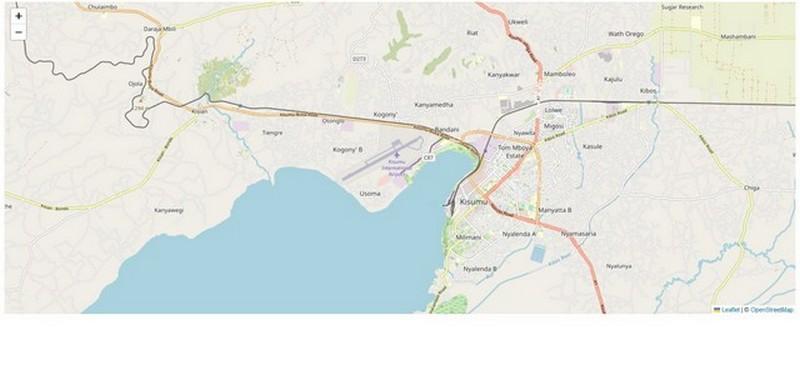
\includegraphics[width=11.11in]{../images/kisumu-leaflet}

What \texttt{L.tileLayer} has done is retrieve the web tiles from the url source provided, and within the dictionary that follows the url, zoom level (\texttt{maxZoom}) and map attribution (\texttt{attribution}) have been provided. When working with leaflet, the dictionary, indicated by the curly braces \texttt{\{\}} houses most of the additional class options other than the key one(s). In this case we used the additional options of \texttt{maxZoom} and \texttt{attribution}. Finally, the method \texttt{addTo} adds the layer to the given map or layer group. Here, our webtile is added to the \texttt{var\ map} which only contains the \texttt{setView} properties.

A very influential person said Kisumu located in Kenya is a town with great potential. How about dispalying it to the whole world to realise it!

\hypertarget{summary-1}{%
\section{Summary}\label{summary-1}}

In this chapter, we created our first leaflet map. Here are a couple of things that you have learnt at the first step of this web mapping journey.

\begin{itemize}
\item
  Browsers read code scripts from top to bottom, much like skimming down a page.
\item
  The styles defined in the CSS style sheet, the \texttt{styles.css} in this case,
  will apply to the HTML elements in the \texttt{map.html} file.
\item
  We use the \texttt{src} attribute to link to a webpage.
\item
  If HTML is the magnificent building, JavaScript acts like a good interior and exterior designer.
\item
  The \texttt{L.map()} class is what initializes the leaflet map.
\end{itemize}

\hypertarget{add-ons}{%
\chapter{Add ons}\label{add-ons}}

Like in the ultimate finale of a series where the episode begins with ``Previously on\ldots{}'', this chapter shall be a continuation of \protect\hyperlink{first-leaflet-map}{Chapter 2}.

So we have a plain looking webmap like the one shown below.

\begin{Shaded}
\begin{Highlighting}[]
\NormalTok{knitr}\SpecialCharTok{::}\FunctionTok{include\_graphics}\NormalTok{(}\FunctionTok{rep}\NormalTok{(}\StringTok{"D:/gachuhi/my{-}leaflet/images/kisumu{-}leaflet.jpg"}\NormalTok{))}
\end{Highlighting}
\end{Shaded}

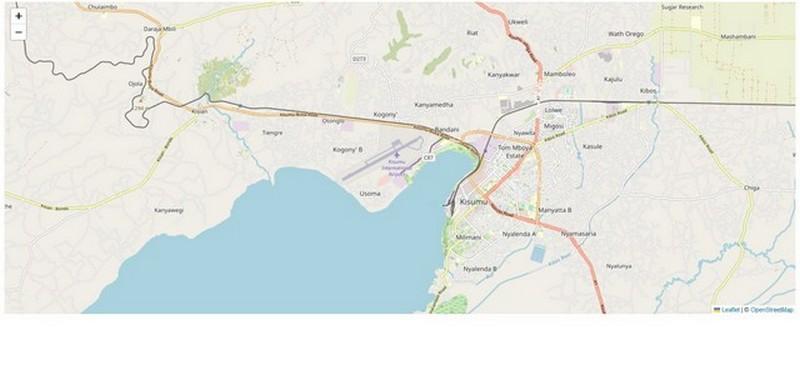
\includegraphics[width=11.11in]{../images/kisumu-leaflet}

However, despite being a cool looking webmap, it offers no sort of information to the viewer except that it is an interactive map interface. In order to pass some information, such as showing the location of Kisumu and \emph{inter alia}, markers are one way of displaying content.

In the last chapter we had last left our \texttt{main.js} file looking like in the image above. Ensure yours is also the same, but we encourage you to explore with other leaflet layers available from \href{https://leaflet-extras.github.io/leaflet-providers/preview/}{here}.

\hypertarget{a-marker}{%
\section{A marker}\label{a-marker}}

Many people could possibly hardly know where Kisumu, is, so lets indicate its location with a simple pin marker. To be more specific, let's pinpoint Kisumu International Airport.

\begin{verbatim}
// Location of Kisumu International Airport
var marker = L.marker([-0.0819301, 34.7260167]).addTo(map);
\end{verbatim}

\begin{Shaded}
\begin{Highlighting}[]
\NormalTok{knitr}\SpecialCharTok{::}\FunctionTok{include\_graphics}\NormalTok{(}\FunctionTok{rep}\NormalTok{(}\StringTok{"D:/gachuhi/my{-}leaflet/images/kisumu{-}international{-}airport.jpg"}\NormalTok{))}
\end{Highlighting}
\end{Shaded}

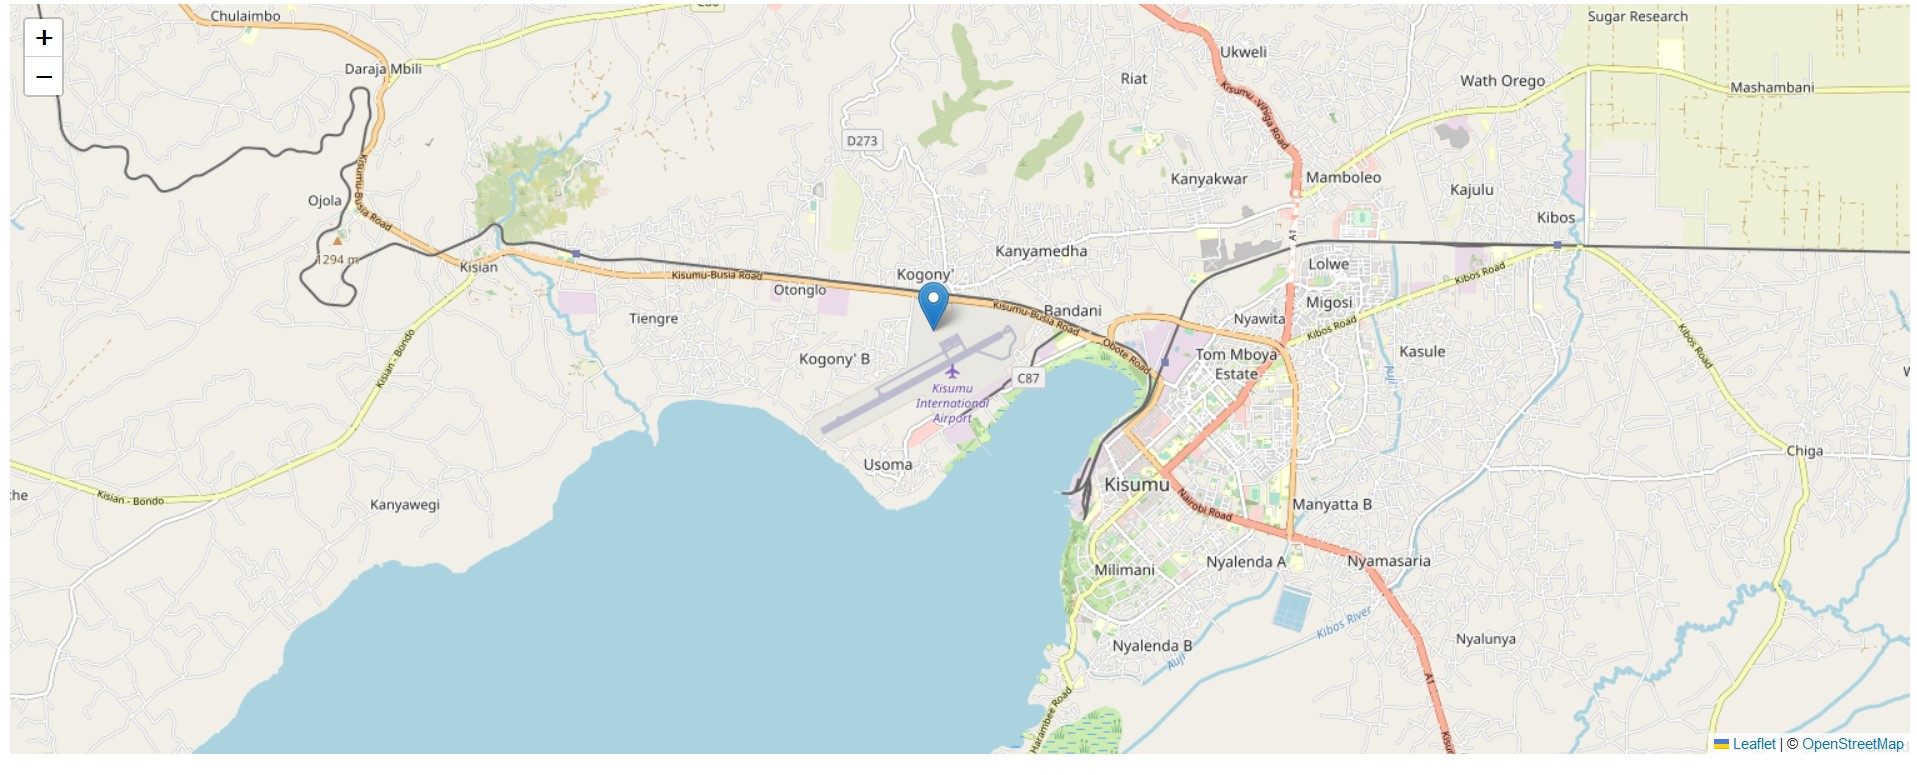
\includegraphics[width=26.62in]{../images/kisumu-international-airport}

As a simple exercise, can you try creating a marker for your home location, not forgetting to change the \texttt{setView} method you had initially started with in this map creating journey?

Alright, we have a marker. But what's so special about it as a lone pin in the middle of somewhere? Let's try to make this marker have some information, otherwise called attributes in GIS. Let's say the attributes we want to add are the name of the airport and other auxillary data.

\hypertarget{a-marker-with-a-popup}{%
\section{A marker with a popup}\label{a-marker-with-a-popup}}

To create popups, leaflet provides the \texttt{bindPopup} method. It is especially easy if you already have a marker variable in place, as in our case.

\begin{verbatim}
// Create popup of Kisumu international Airport
marker.bindPopup("Kisumu International Airport.").openPopup();
\end{verbatim}

\begin{Shaded}
\begin{Highlighting}[]
\NormalTok{knitr}\SpecialCharTok{::}\FunctionTok{include\_graphics}\NormalTok{(}\FunctionTok{rep}\NormalTok{(}\StringTok{"D:/gachuhi/my{-}leaflet/images/kisumu{-}airport{-}popup.jpg"}\NormalTok{))}
\end{Highlighting}
\end{Shaded}

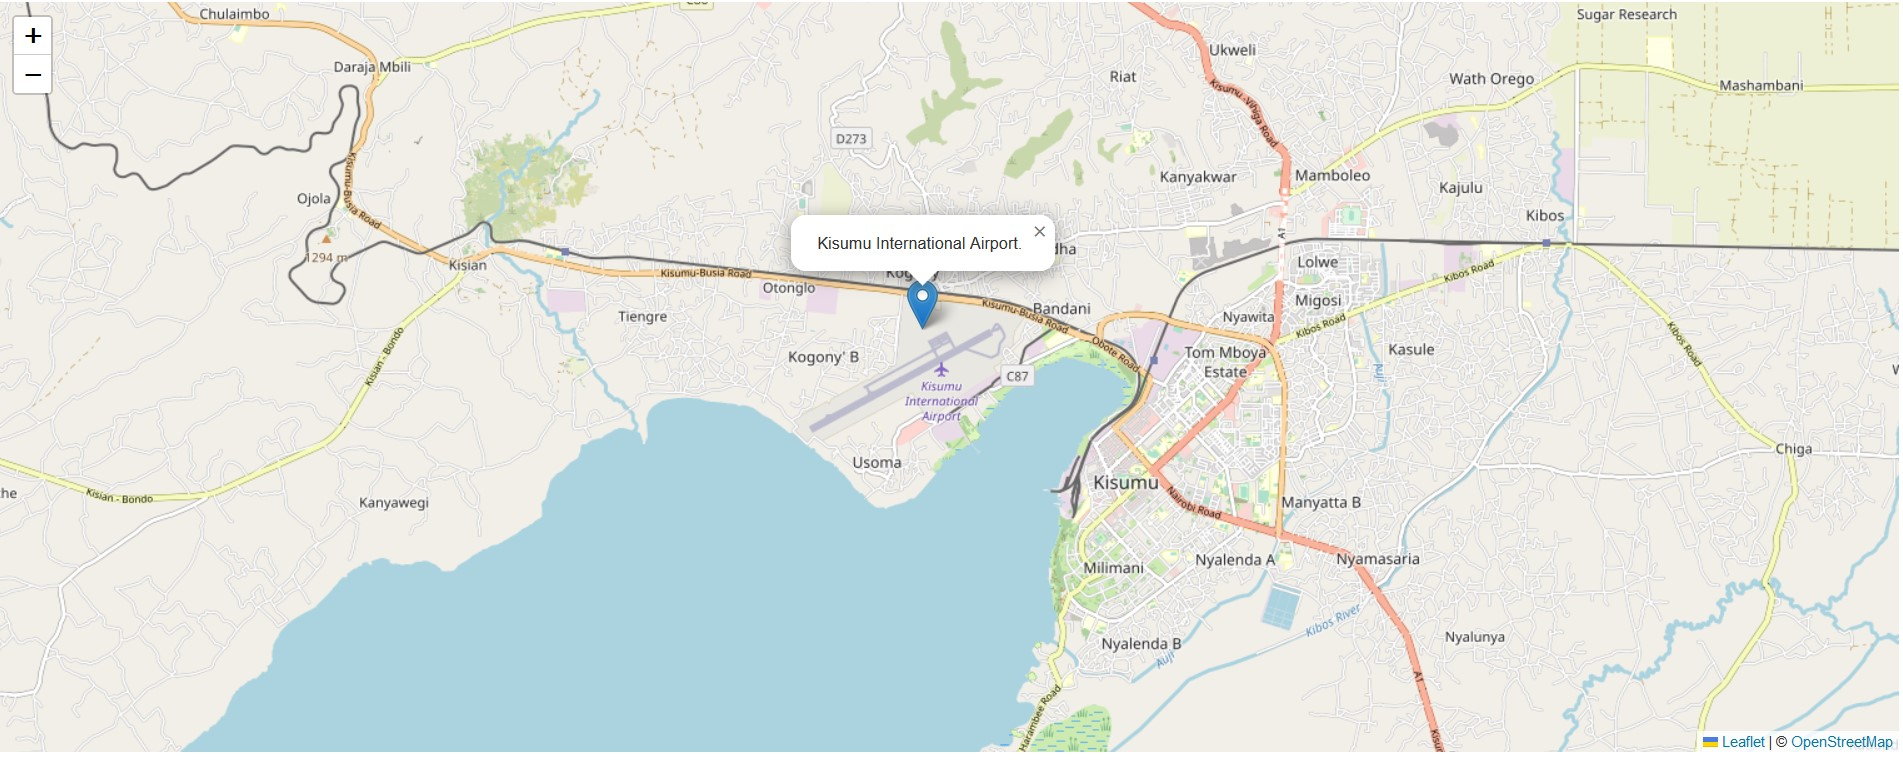
\includegraphics[width=26.43in]{../images/kisumu-airport-popup}

What has just happened is that \texttt{bindPopup} binds the popup content-- ``Kisumu International Airport'' to the marker. The following \texttt{openPopup} method chained to the method \emph{opens} the popup at that specified latitude longitude. If you remove, or comment \texttt{//} out the \texttt{popUp} method, you will have to click the marker to see the popup content. Try it out.

Markers can also work with HTML elements, such as when you want to display additional metadata, say the owner of the place, size of land et cetera. In the below case, we have added the lat-lon coordinates of Kisumu airport location. I would advise not to include lengthy information in an HTML marker element.

\begin{verbatim}
// With html content
marker.bindPopup("<br>Name: Kisumu International Airport</br><br>Latitude: -0.0819301</br><br>Longitude: 34.7260167</br>").openPopup();
\end{verbatim}

\begin{Shaded}
\begin{Highlighting}[]
\NormalTok{knitr}\SpecialCharTok{::}\FunctionTok{include\_graphics}\NormalTok{(}\FunctionTok{rep}\NormalTok{(}\StringTok{"D:/gachuhi/my{-}leaflet/images/marker{-}html.jpg"}\NormalTok{))}
\end{Highlighting}
\end{Shaded}

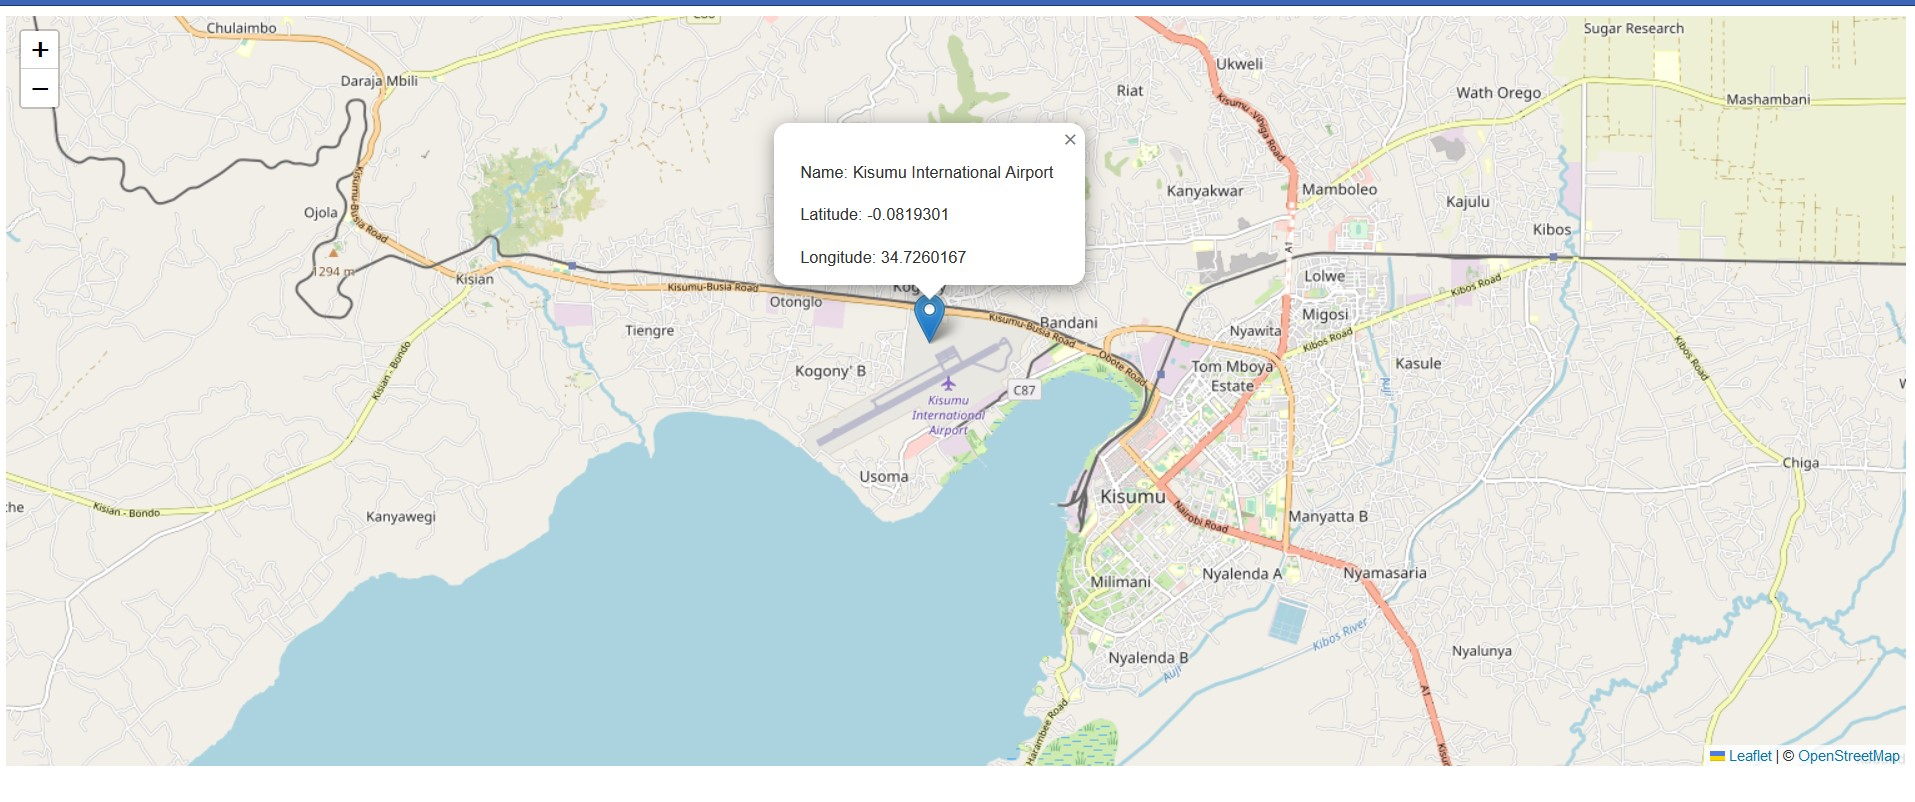
\includegraphics[width=26.6in]{../images/marker-html}

\hypertarget{different-markers-and-popups}{%
\section{Different markers and popups}\label{different-markers-and-popups}}

So far you have seen pin markers, but there are also other kinds of markers, such as circles and rectangles. Unlike the pin markers we have been experimenting with, these other markers require additional options, such as radius for circle and lat-long coordinates for rectangles. Let's have a go with each type.

Starting with a circle, let's start by inserting a circle to show the location of Kisumu Museum.

\begin{verbatim}
// Circle over Kisumu Museum
var circle = L.circle([-0.107637, 34.7435975]).setRadius(2000).addTo(map);
\end{verbatim}

\begin{Shaded}
\begin{Highlighting}[]
\NormalTok{knitr}\SpecialCharTok{::}\FunctionTok{include\_graphics}\NormalTok{(}\FunctionTok{rep}\NormalTok{(}\StringTok{"D:/gachuhi/my{-}leaflet/images/kisumu{-}museum{-}circle.jpg"}\NormalTok{))}
\end{Highlighting}
\end{Shaded}

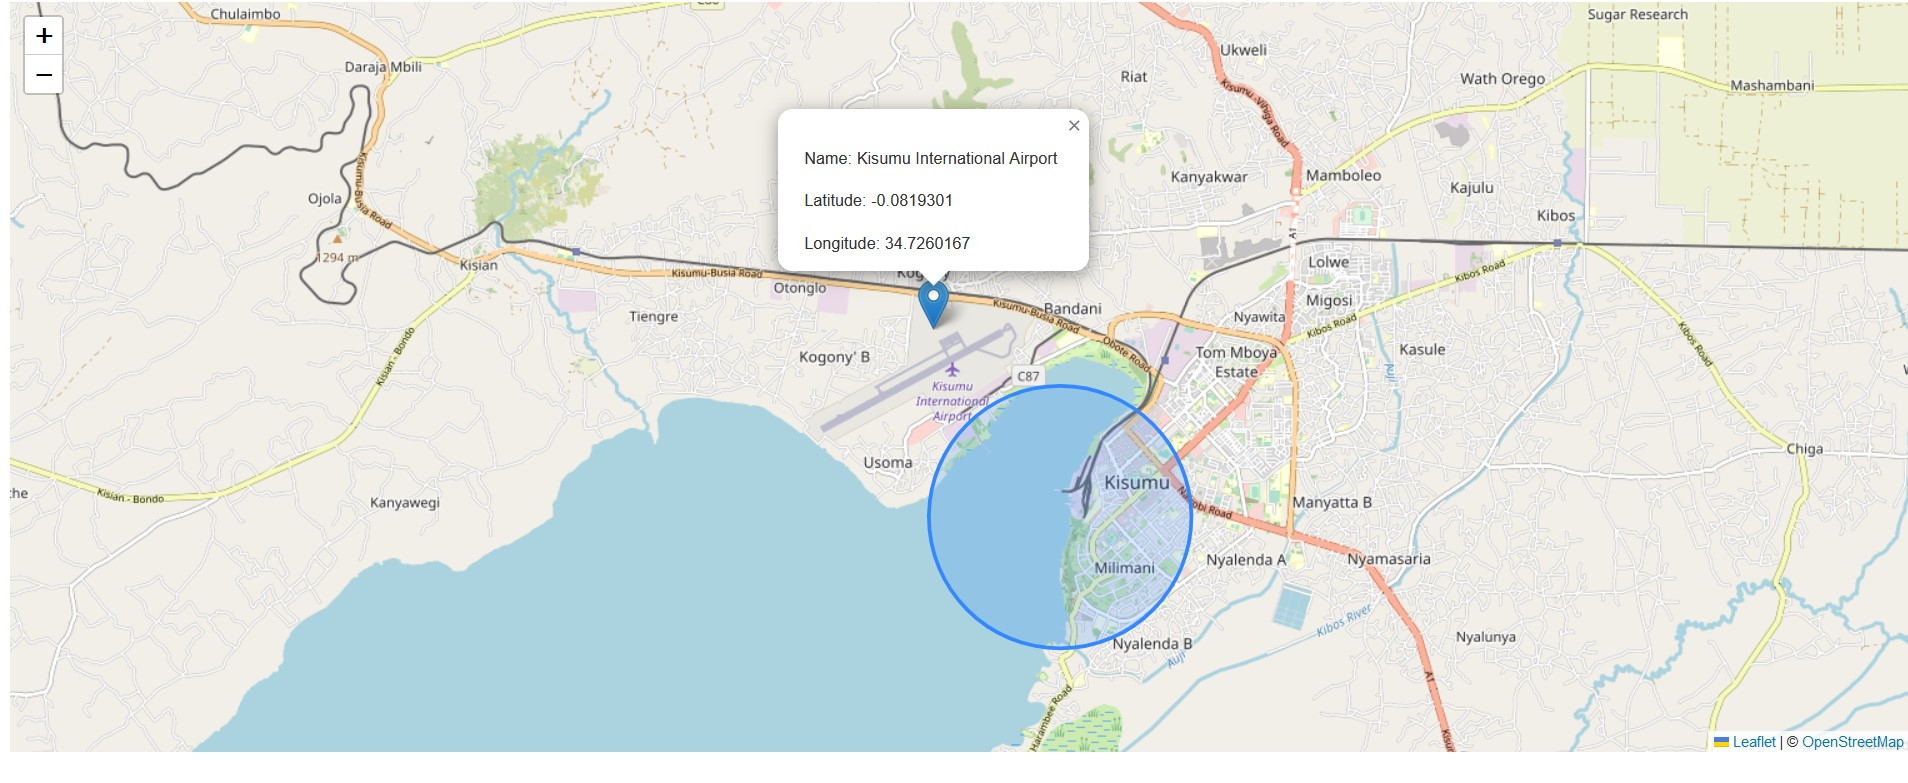
\includegraphics[width=26.5in]{../images/kisumu-museum-circle}

The below code will also create a slightly similar circle marker, the only difference is that in the preceding one we didn't insert \texttt{\{options\}} and we set radius using the \texttt{setRadius} method. In the second one below, we have been very specific in what we want --our specifications going into the curly brackets \{\} before eventually adding the circle marker to our map. Brackets in JavaScript denote \href{https://flexiple.com/javascript/javascript-dictionary/}{dictionaries}. Dictionaries in JavaScript and even in python are used to denote key-value pairs.

\begin{verbatim}
var circle = L.circle([-0.107637, 34.7435975], {
    color: 'blue',
    fillColor: 'blue',
    fillOpacity: .5,
    radius: 2000
}).addTo(map);
\end{verbatim}

As we had mentioned earlier, other marker elements such as circles and rectangles can have popups attached to them. Ready for something cool? We will attach a popup into our circle. Not just any other ordinary hard coded popup but one which relies on other Leaflet JavaScript methods to generate an output. In our case, we want a pop up that shows the radius of our circle, without us typing it out into the code.

\begin{verbatim}
// Circle marker pop up for Kisumu Museum
var getRadius = circle.getRadius();
circle.bindPopup("Radius is: " + getRadius.toString() + " metres");
\end{verbatim}

In our above code, \texttt{getRadius} gets the radius of our circle marker. \texttt{bindPopup} as has already been explained before \emph{binds} the popup content to our circle marker. But there is a catch. The variable \texttt{getRadius} is used to print out the results, which is 2000 of course. However, \texttt{bindPopup} only understands strings so we convert our variable result to a string using \texttt{toString()}. We also added other strings to give the popup a wholesome result that is understandable to every Tom, Dick, Harry and Harriet.

\begin{Shaded}
\begin{Highlighting}[]
\NormalTok{knitr}\SpecialCharTok{::}\FunctionTok{include\_graphics}\NormalTok{(}\FunctionTok{rep}\NormalTok{(}\StringTok{"D:/gachuhi/my{-}leaflet/images/circle{-}radius.jpg"}\NormalTok{))}
\end{Highlighting}
\end{Shaded}

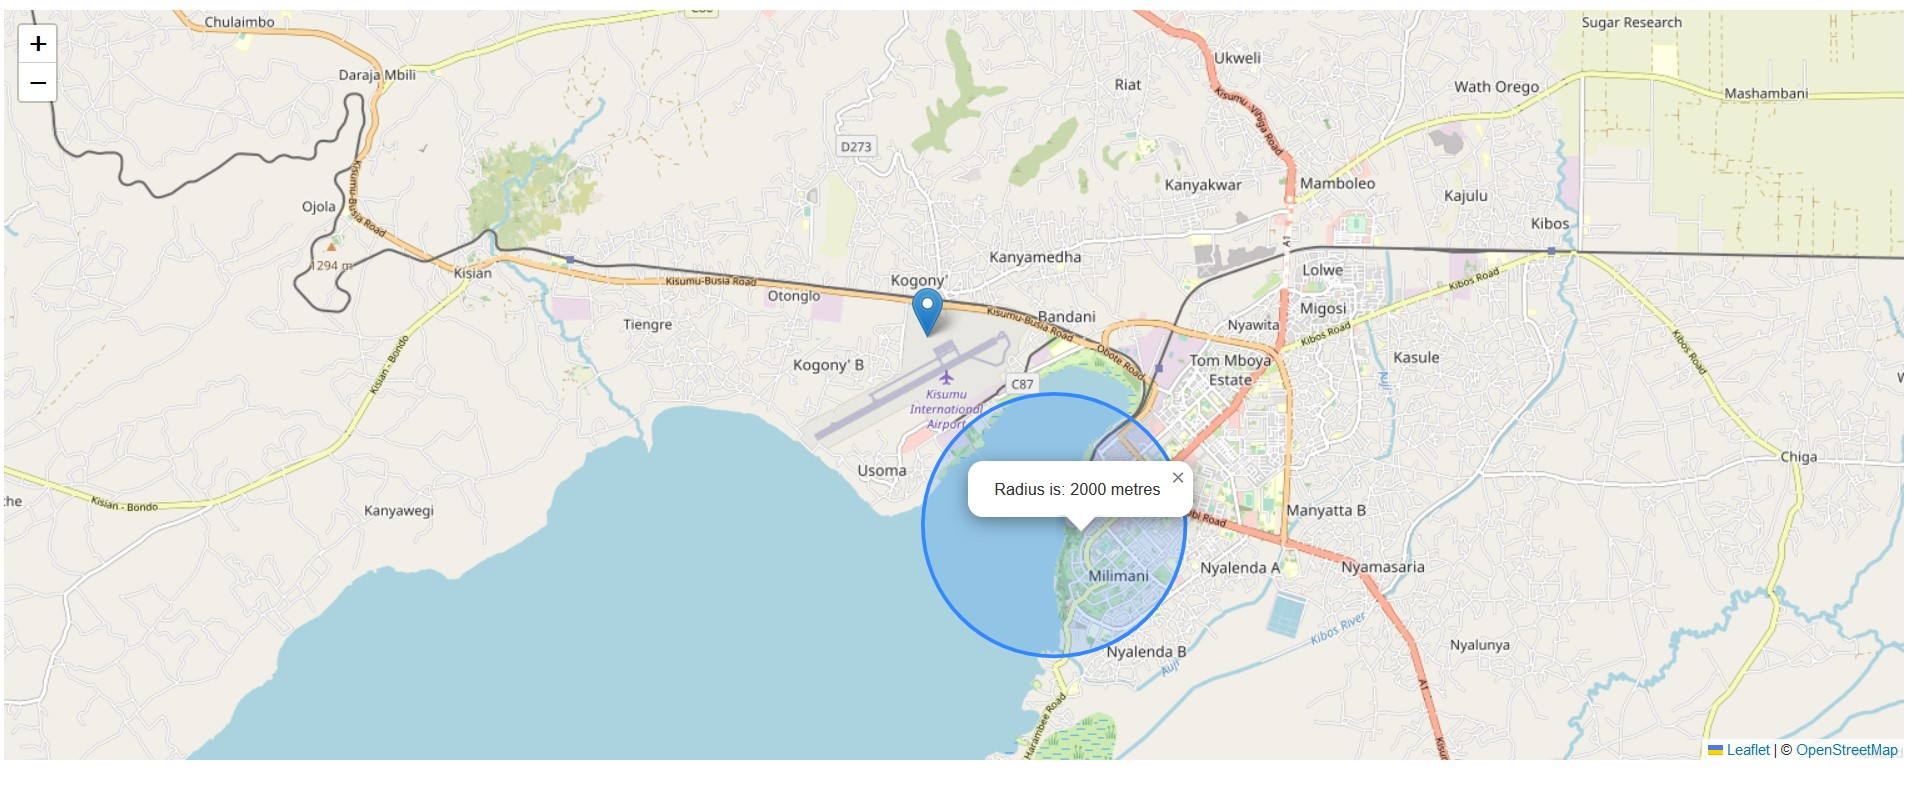
\includegraphics[width=26.57in]{../images/circle-radius}

Finally, let's try with a rectangle. Actually, leaflet allows us to create polygons, and with a polygon --at least in leaflet, you can also create rectangles. Let's work with the polygon class instead.

Copy the following coordinates.

\begin{verbatim}
// Draw rectangle around Kisumu Wildlife Impala Park
var impalaParkCoordinates = [
    [-0.1144753, 34.743418],
    [-0.115097, 34.745242],
    [-0.114238, 34.745071],
    [-0.114002, 34.746101],
    [-0.115054, 34.746787],
    [-0.115998, 34.745586],
    [-0.118444, 34.746208],
    [-0.121255, 34.744684]
]
\end{verbatim}

Now using the \texttt{L.polygon} class and a few optional parameters, let's showcase where the Kisumu Wildlife Impala Park is situated.

\begin{verbatim}
// Create a polygon using the above coordinates
var impalaParkPolygon = L.polygon(impalaParkCoordinates, {
    color: 'brown',
    fillOpacity: 0.4
}).addTo(map);
\end{verbatim}

You will notice that the Kisumu Museum circle overlaps the location of the Kisumu Impala Park but that is no problem. We will make our popup content appear by default as soon as you load the map. Just like we did for the circle marker, we will make our popup content rely on another variable, in this case \texttt{getCenter} which gets the centroid coordinates of our polygon. We were looking for something cooler such as \texttt{getArea} in Leaflet, one that automatically prints out the area of a polygon in a popup. Unfortunately, we were unable to find it.

\begin{verbatim}
// Add popup to the polygon of Kisumu Impala Park
var getCenter = impalaParkPolygon.getCenter();
impalaParkPolygon.bindPopup("Centre is at Lat-Lon: " + getCenter.toString()).openPopup();
\end{verbatim}

If you find the circle marker radius as an obstraction you can comment out it and its dependancies using \texttt{//}.

\begin{Shaded}
\begin{Highlighting}[]
\NormalTok{knitr}\SpecialCharTok{::}\FunctionTok{include\_graphics}\NormalTok{(}\FunctionTok{rep}\NormalTok{(}\StringTok{"D:/gachuhi/my{-}leaflet/images/polygon{-}marker.jpg"}\NormalTok{))}
\end{Highlighting}
\end{Shaded}

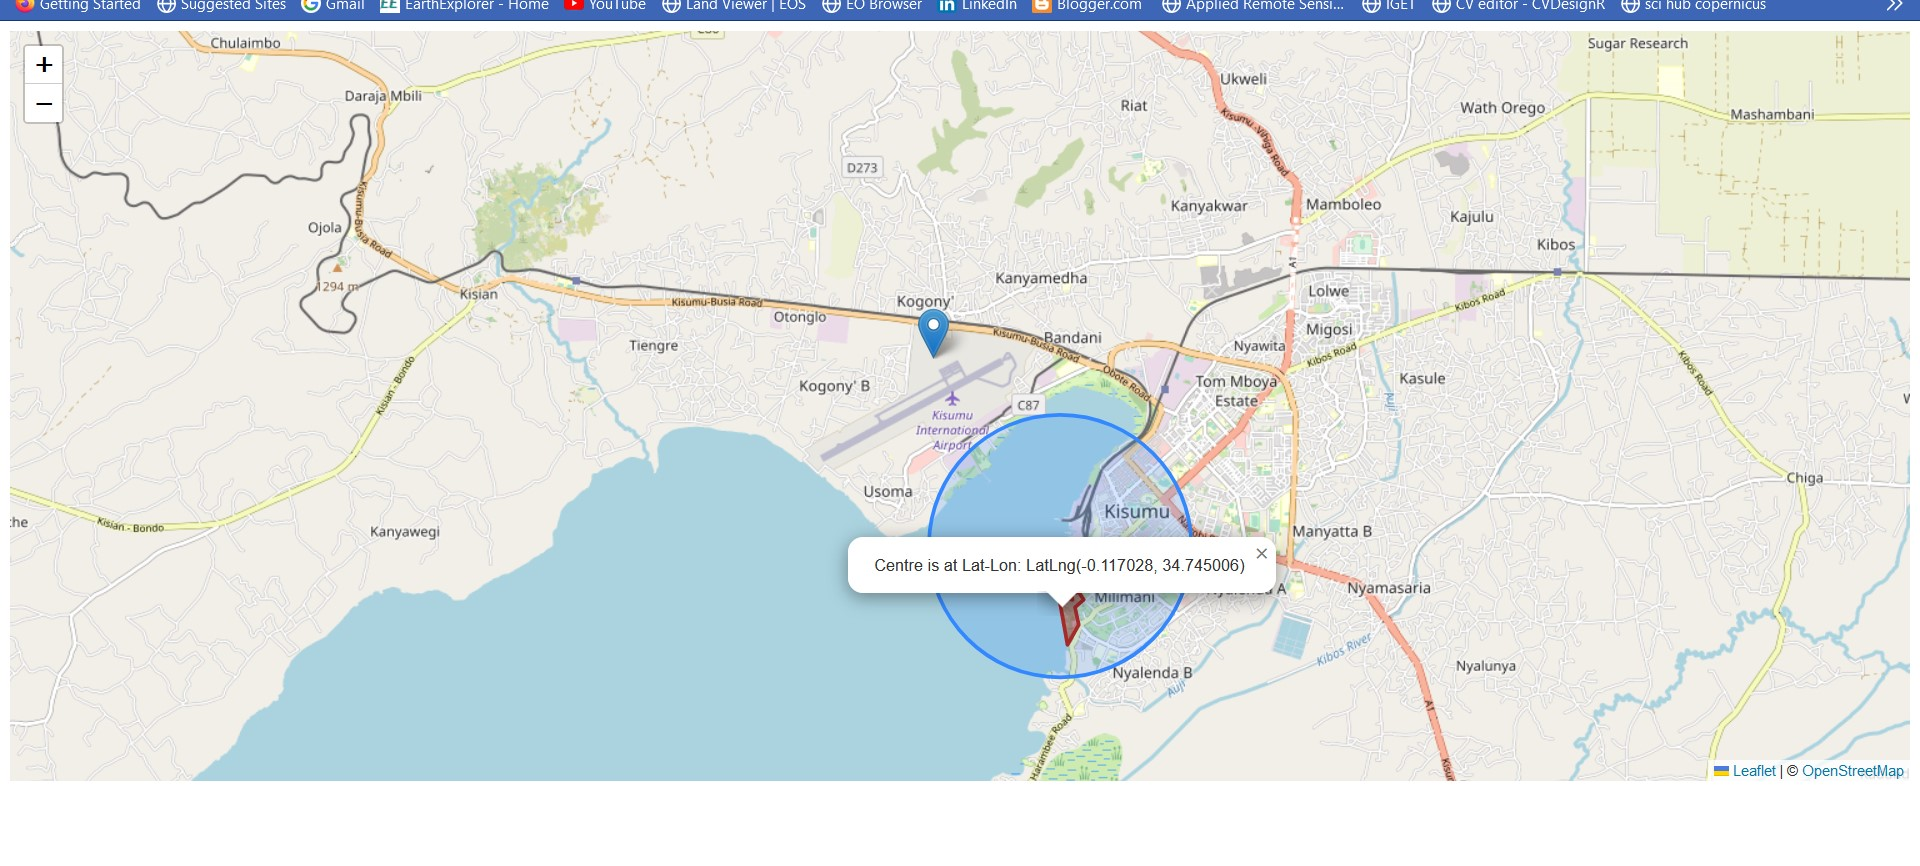
\includegraphics[width=26.67in]{../images/polygon-marker}

You can get the files used in this exercise \href{https://github.com/sammigachuhi/my-leaflet-project/tree/main/my-leaflet-code/chapter-3-markers}{here}.

\hypertarget{summary-2}{%
\section{Summary}\label{summary-2}}

This chapter took you further in enriching the content that can be displayed in a webmap. You have seen that a webmap can offer far more useful information than just mere markers and symbols on a web canvas. Popups are one way of displaying information, and they too can be customized further. Through the practicals in this chapter, you have learnt the following:

\begin{itemize}
\item
  To create popups in leaflet, we use the \texttt{bindPopup} method.
\item
  \texttt{openPopup} automatically opens the popups once the leaflet map is loaded. They only disappear once you close them.
\item
  Markers can also work with HTML elements.
\item
  Apart from location pins, markers can also be circles and rectangles.
\item
  There exist methods in leaflet that can automatically parse out information in popups without requiring any hardcoding from the programmer. For example, we used \texttt{getRadius} to display the circle radius in the popup without necessarily typing it out in the \texttt{bindPopup} method.
\end{itemize}

You comment out JavaScript code with \texttt{//}!

\hypertarget{embedding-leaflet-map-to-an-external-website}{%
\chapter{Embedding leaflet map to an external website}\label{embedding-leaflet-map-to-an-external-website}}

\hypertarget{a-website-with-a-sense-of-direction}{%
\section{A website with a sense of direction}\label{a-website-with-a-sense-of-direction}}

Now, we have succeeded in making a stand alone leaflet map. However, we want to do something that will quickly upscale you from a novice to a pro. That is, placing the leaflet map into a website.

An example of what we want is shown below, which is a snapshot from the \href{https://data.humdata.org/dataset/cod-ab-ken}{HDX website}.

\begin{Shaded}
\begin{Highlighting}[]
\NormalTok{knitr}\SpecialCharTok{::}\FunctionTok{include\_graphics}\NormalTok{(}\FunctionTok{rep}\NormalTok{(}\StringTok{"D:/gachuhi/my{-}leaflet/images/webmap{-}in{-}web.jpg"}\NormalTok{))}
\end{Highlighting}
\end{Shaded}

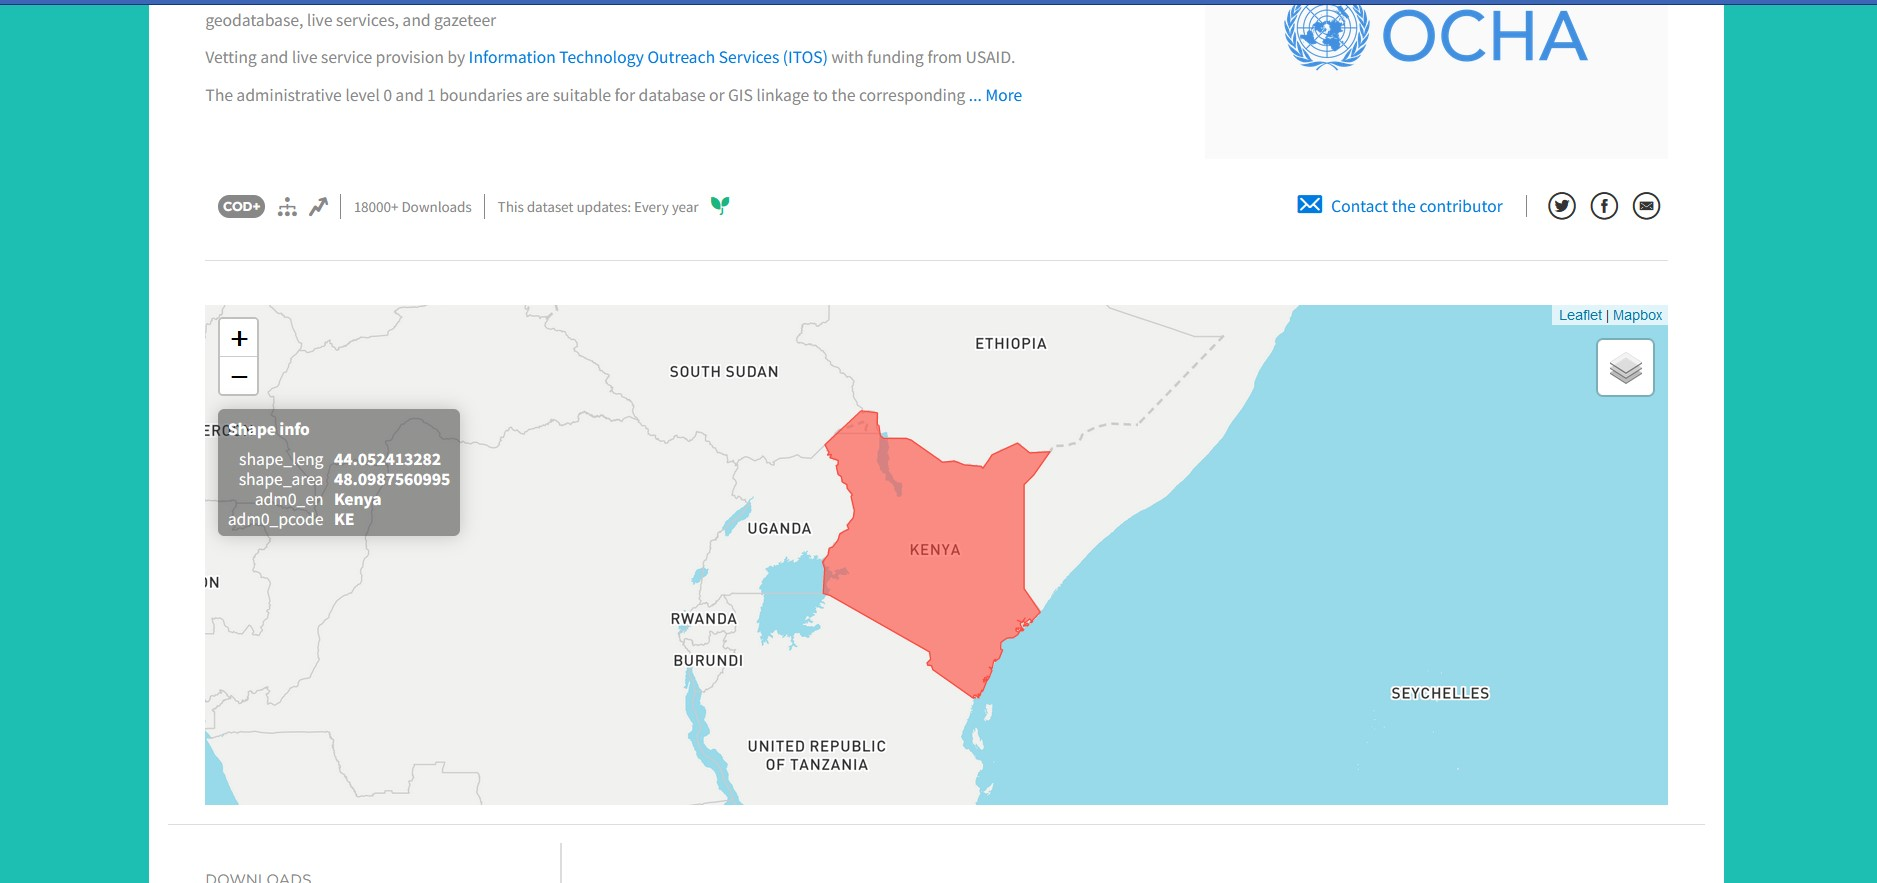
\includegraphics[width=26.07in]{../images/webmap-in-web}

For this exercise, we shall embed a leaflet map to a simple HTML webpage. This webpage doesn't look grand, but it serves the purpose of our exercise. Let's get on to it. Here are the \href{https://github.com/sammigachuhi/my-leaflet-project/tree/main/my-leaflet-code/chapter-4-embed-leaflet-website}{files}.

\hypertarget{the-html-webpage}{%
\section{The HTML webpage}\label{the-html-webpage}}

Create a HTML page with the following code.

\begin{verbatim}
<!DOCTYPE html>
<html lang="en">
    <head>
        <title>Pro-GMO Alliance</title>
        <meta charset="utf-8">
        <link rel="stylesheet" href="example-styles.css">
        <link rel="stylesheet" href="https://unpkg.com/leaflet@1.9.3/dist/leaflet.css"
        integrity="sha256-kLaT2GOSpHechhsozzB+flnD+zUyjE2LlfWPgU04xyI="
        crossorigin=""/>
        <script src="https://unpkg.com/leaflet@1.9.3/dist/leaflet.js"
        integrity="sha256-WBkoXOwTeyKclOHuWtc+i2uENFpDZ9YPdf5Hf+D7ewM="
        crossorigin=""></script>
    </head>
    <body>
    <div id="div-for-article">
        <article id="introduction">
            <h2>Introduction</h2>
            <q>Sed ut perspiciatis unde omnis iste natus error sit voluptatem accusantium 
            doloremque laudantium, totam rem aperiam, eaque ipsa quae ab illo inventore veritatis et 
            quasi architecto beatae vitae dicta sunt explicabo. Nemo enim ipsam voluptatem quia voluptas 
            sit aspernatur aut odit aut fugit, sed quia consequuntur magni dolores eos qui ratione 
            voluptatem sequi nesciunt. Neque porro quisquam est, qui dolorem ipsum quia dolor sit amet, 
            consectetur, adipisci velit, sed quia non numquam eius modi tempora incidunt ut labore et 
            dolore magnam aliquam quaerat voluptatem. Ut enim ad minima veniam, quis nostrum exercitationem 
            ullam corporis suscipit laboriosam, nisi ut aliquid ex ea commodi consequatur? Quis autem 
            vel eum iure reprehenderit qui in ea voluptate velit esse quam nihil molestiae consequatur, 
            vel illum qui dolorem eum fugiat quo voluptas nulla pariatur?</q>
        </article>
    </div>
    <div id="div-for-section">
        <section id="Products">
            <div class="row">
                <h2>Our Products</h2>
                <div class="column">
                  <img src="https://images.unsplash.com/photo-1632125941710-35a9d2fcc7ce?ixlib=rb-4.0.3&ixid=MnwxMjA3fDB8MHxwaG90by1wYWdlfHx8fGVufDB8fHx8&auto=format&fit=crop&w=1170&q=80" alt="Maize" style="width:100%">
                </div>
                <div class="column">
                    <img src="https://images.unsplash.com/photo-1595615636850-3292eb0a95b0?ixlib=rb-4.0.3&ixid=MnwxMjA3fDB8MHxwaG90by1wYWdlfHx8fGVufDB8fHx8&auto=format&fit=crop&w=1170&q=80" alt="Sunflower" style="width:100%">
                  </div>
                <div class="column">
                  <img src="https://images.unsplash.com/photo-1600333859399-228aa03f7dba?ixlib=rb-4.0.3&ixid=MnwxMjA3fDB8MHxwaG90by1wYWdlfHx8fGVufDB8fHx8&auto=format&fit=crop&w=1170&q=80" alt="Potato" style="width:100%">
                </div>
                <div class="column">
                  <img src="https://images.unsplash.com/photo-1630145398476-853543b02843?ixlib=rb-4.0.3&ixid=MnwxMjA3fDB8MHxwaG90by1wYWdlfHx8fGVufDB8fHx8&auto=format&fit=crop&w=1167&q=80" alt="Cotton" style="width:100%">
                </div>
              </div>
        </section>
    </div>
    <div>
        <br>
        <h2>Our Branches</h2>
        <br>
    </div>
      <div class="container">
        <div id="map">
          <script src="example-main.js"></script>
        </div>
        <div class="text">
          <h1>Address</h1>
          <p>
            P.O. Box 55044, Nakuru
        </p>
        </div>
      </div>
    </body>
</html>
\end{verbatim}

Since this is a geospatial book, we shall not go through every line of the HTML code above. It just a webpage containing some text, some pictures and a webmap. The webmap is the centre of our interest in this chapter. How do we create a Leaflet map, of which we know how to do, and fit it inside an existing webpage?

Before we head there, let's insert the CSS file, which looks like this.

\begin{verbatim}
/* Three image containers (use 25% for four, and 50% for two, etc) */
.column {
    float: left;
    width: 33.33%;
    padding: 5px;
  }
  
  /* Clear floats after image containers */
  .row::after {
    content: "";
    clear: both;
    display: table;
  }


/* Styling the map */
  .container {
    display: flex;
    align-items: center;
    justify-content: center
  }

#map {
    height: 300px; 
    width: 90%
}

.text {
    font-size: 15px;
    padding-left: 20px;
}
\end{verbatim}

\hypertarget{the-leaflet-javascript-code-for-our-website}{%
\section{The leaflet JavaScript code for our website}\label{the-leaflet-javascript-code-for-our-website}}

Back to the leaflet map of our dummy Pro-GMO Alliance webpage. How did we put the leaflet in there? Nothing complicated, just inserting the same leaflet code, with some additional JavaScript and calling it within the HTML file with \texttt{\textless{}script\ src="example-main.js"\textgreater{}\textless{}/script\textgreater{}}. The Javascript file used is shown below.

\begin{verbatim}
var map = L.map('map').setView([-0.302765, 36.146147], 12);

L.tileLayer('https://tile.openstreetmap.org/{z}/{x}/{y}.png', {
    maxZoom: 19,
    attribution: '&copy; <a href="http://www.openstreetmap.org/copyright">OpenStreetMap</a>'
}).addTo(map);

var branches = [
    ["Potatoes",-0.328858, 36.008474],
    ["Maize",-0.302765, 36.146147],
    ["Sunflower",-0.224832, 36.159880],
    ["Cotton", -0.214189, 36.135847]
    ];

for (var i = 0; i < branches.length; i++) {
    marker = new L.marker([branches[i][1], branches[i][2]])
        .bindPopup(branches[i][0])
        .addTo(map);
}
\end{verbatim}

The only new thing in the above script is the \texttt{for} loop. In JavaScript, the \texttt{for} loop is used to iterate over items. In this case, and remembering that indexing in arrays begins from 0, the marker popups will read the latitudes and longitudes which are at index 1 and 2 respectively. The lat-lon are indicated by \texttt{({[}branches{[}i{]}{[}1{]},\ branches{[}i{]}{[}2{]}{]})}. The popup strings, which appear as the first elements in the \texttt{branches} array, are at index 0. The popup strings are indicated by \texttt{branches{[}i{]}{[}0{]}}. At the end of the chain the markers are added to the map with \texttt{.addTo}.

Alright. How about the keyword \texttt{new}?

The \texttt{new} keyword is a constructor. That is, it creates an empty object. Many instances of the variable \texttt{marker} can be created from the instance of \texttt{new} object. For more information on the \texttt{new} keyword constructor, see this \href{https://www.programiz.com/javascript/constructor-function}{website}. Be rest assured that the \texttt{new} keyword isn't mandatory to make the webmap to work in our case but its helpful to add another JavaScript trick to your hat.

Below is a snapshot of how the dummy Pro-GMO website looks like with our newly embedded webmap.

\begin{Shaded}
\begin{Highlighting}[]
\NormalTok{knitr}\SpecialCharTok{::}\FunctionTok{include\_graphics}\NormalTok{(}\FunctionTok{rep}\NormalTok{(}\StringTok{"D:/gachuhi/my{-}leaflet/images/embedded.jpg"}\NormalTok{))}
\end{Highlighting}
\end{Shaded}

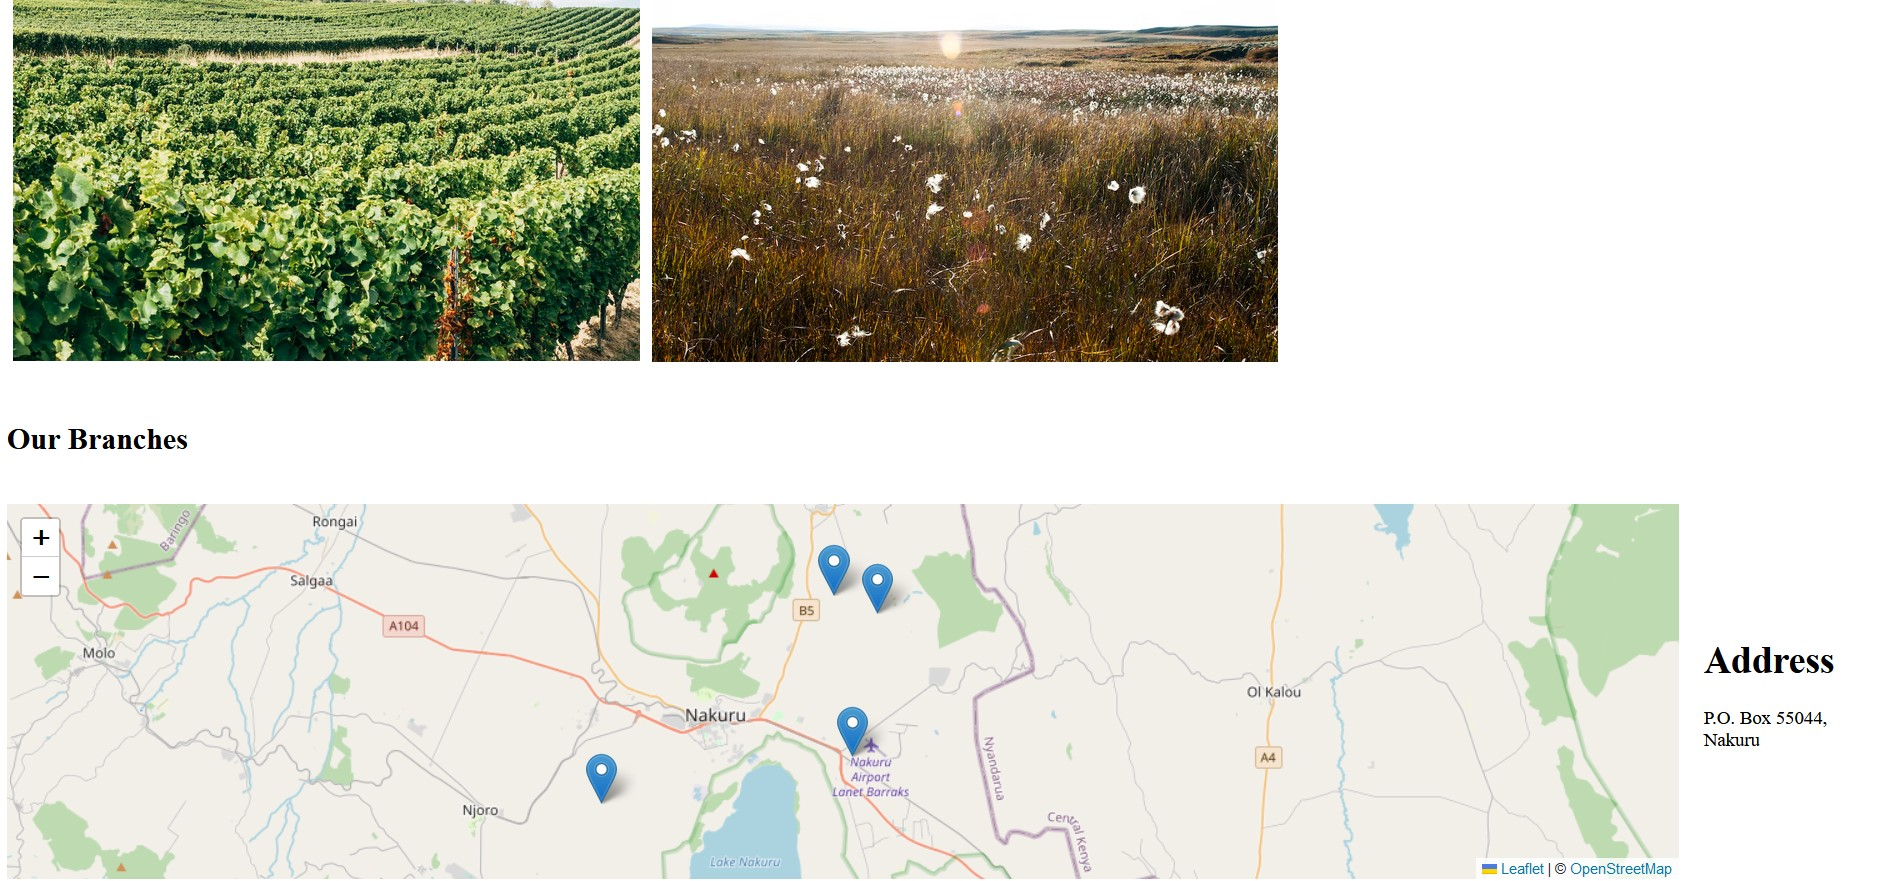
\includegraphics[width=26.21in]{../images/embedded}

``How are we able to align the webmap to the left and also make other text stand aside to it?'' This is all thanks to the CSS property \texttt{display:\ flex}. \texttt{display} is a CSS property that deals with how HTML elements are displayed.
This property aligns the element to fill or shrink according to the space available within its assigned portion in the webpage. On the other hand, the CSS property \texttt{padding-left} just creates space all around the element, thus creating a neat space between the leaflet map and the address text. Removing this will just make the address text and the leaflet map touch each other edge to edge. The inspiration to use all these CSS properties and values in placing HTML elements side-by-side enamated from this \href{https://www.w3docs.com/snippets/css/how-to-vertically-align-text-next-to-an-image.html?utm_source=pocket_saves}{example}.

Having done the above, you can consider you are as good a Leaflet mapper to undertake any task!

\hypertarget{summary-3}{%
\section{Summary}\label{summary-3}}

This chapter has introduced you on how you can use CSS to customize the appearance and positioning of your webmap. You have also encountered the use of \texttt{for} loop in JavaScript code to retrieve geospatial information, particularly from arrays. Here are brief notes of your take aways from this chapter.

\begin{itemize}
\item
  Leaflet maps can be embedded inside a website as demonstrated in the dummy Pro-GMO webpage.
\item
  One can use \texttt{for} loops to iterate over elements from an array and retrieve geospatial information. In this chapter, the \texttt{for} loop was used to retrieve both latitude-longitude coordinates and text from the \texttt{branches} array variable.
\item
  We can use CSS elements, such as \texttt{display} and \texttt{padding-left} to position and define how webmap shall be displayed on our webpage.
\end{itemize}

\hypertarget{using-geojson-in-leaflet}{%
\chapter{Using GeoJSON in Leaflet}\label{using-geojson-in-leaflet}}

\hypertarget{creating-a-.geojson-file}{%
\section{\texorpdfstring{Creating a \texttt{.geojson} file}{Creating a .geojson file}}\label{creating-a-.geojson-file}}

So far, we have created a leaflet map, added some aesthetics such as markers, and even embedded a map into a dummy website. Alright, the website wasn't even close to good, but the methodology should be the same when working with other fully functional and better looking websites. That may be enough to give you confidence to start as a webmapper, but not so fast! There is always, and will be some more things to learn and in this case I would like to introduce another format of storing geospatial information. The use of \texttt{.geojson} files.

\hypertarget{what-are-.geojson-files}{%
\section{\texorpdfstring{What are \texttt{.geojson} files?}{What are .geojson files?}}\label{what-are-.geojson-files}}

\texttt{.geojson} files, according to the GIS leader ESRI, are an \href{https://doc.arcgis.com/en/arcgis-online/reference/geojson.htm}{open standard geospatial data interchange format} that represents simple geographic features and their nonspatial attributes. GeoJSON is based on the JavaScript Object Notation (JSON) file format which is a lightweight data exchange format that is easily interpretable by both man and machine. In very few instances can any format please both sides of the divide but JSON does, and this \href{https://www.oracle.com/ke/database/what-is-json/}{site} provides examples. Anyway, just like you can tell from the name, it is also based from the JavaScript programming language. If you have worked with JavaScript before, it looks very much like a data format based on dictionaries. In essence, JSON is a large dictionary holding other \emph{dictionaries} of data within it. A GeoJSON is a JSON file that follows a certain structure and has spatial index and geometry specifications in it. See this \href{https://datascience.aero/geospatial-data-representation-the-geojson-format/}{website} for a geojson example.

An example of a GeoJSON file format structure is shown below:

\begin{verbatim}
{
  "type": "FeatureCollection",
  "features": [
    {
      "type": "Feature",
      "properties": {
        "City": "Nairobi",
        "Population": "4, 300, 000"
      },
      "geometry": {
        "coordinates": [
          36.80617598261199,
          -1.2868825246637812
        ],
        "type": "Point"
      }
    },
    {
      "type": "Feature",
      "properties": {
        "City": "Kisumu",
        "Population": "610, 082"
      },
      "geometry": {
        "coordinates": [
          34.738718987625106,
          -0.10390483386935045
        ],
        "type": "Point"
      }
    },
    ---snip----
\end{verbatim}

Below is an example of a \href{https://www.oracle.com/ke/database/what-is-json/}{json file structure}.

\begin{verbatim}
{

"Influencers" :   [ 
{
 "name" : "Jaxon", 
 "age" : 42, 
 "Works At" : "Tech News"
}

{
 "name" : "Miller", 
 "age" : 35
 "Works At" : "IT Day"
}

] 
}
\end{verbatim}

\hypertarget{why-geojson}{%
\section{\texorpdfstring{Why \texttt{geojson}?}{Why geojson?}}\label{why-geojson}}

Yours truly could be wrong, but one advantage of \texttt{geojson} and \texttt{json} is that it's minimal on size (sometimes) and is more portable than shapefiles. Shapefiles are dependent on other data formats that accompany it, such as \texttt{.shx}, \texttt{.dbf}, \texttt{.prj} and others that provide geospatial orientation, metadata, attributes and others. GeoJSON and JSON formats will come as standalone and holding the same amount of data.

So when do I use shapefiles vis a vis GeoJson? If you want to work with geospatial data in a web interface, \texttt{geojson} is the way to go. Period.

\hypertarget{creating-a-geojson-file}{%
\section{Creating a geojson file}\label{creating-a-geojson-file}}

``Creating a geojson file with several dictionaries in it looks very intimidating. No hope of creating one without errors.'' You may think to yourself. Precisely, but luckily, we have the \href{https://geojson.io/\#map=2/0/20}{geojson.io} website that does the heavylifting for us. We shall head over to it and create a \texttt{geojson} file of some cities and their population.

First, of all, the website looks like this, a cool global map powered by Mapbox.

\begin{Shaded}
\begin{Highlighting}[]
\NormalTok{knitr}\SpecialCharTok{::}\FunctionTok{include\_graphics}\NormalTok{(}\FunctionTok{rep}\NormalTok{(}\StringTok{"D:/gachuhi/my{-}leaflet/images/mapbox{-}front.jpg"}\NormalTok{))}
\end{Highlighting}
\end{Shaded}

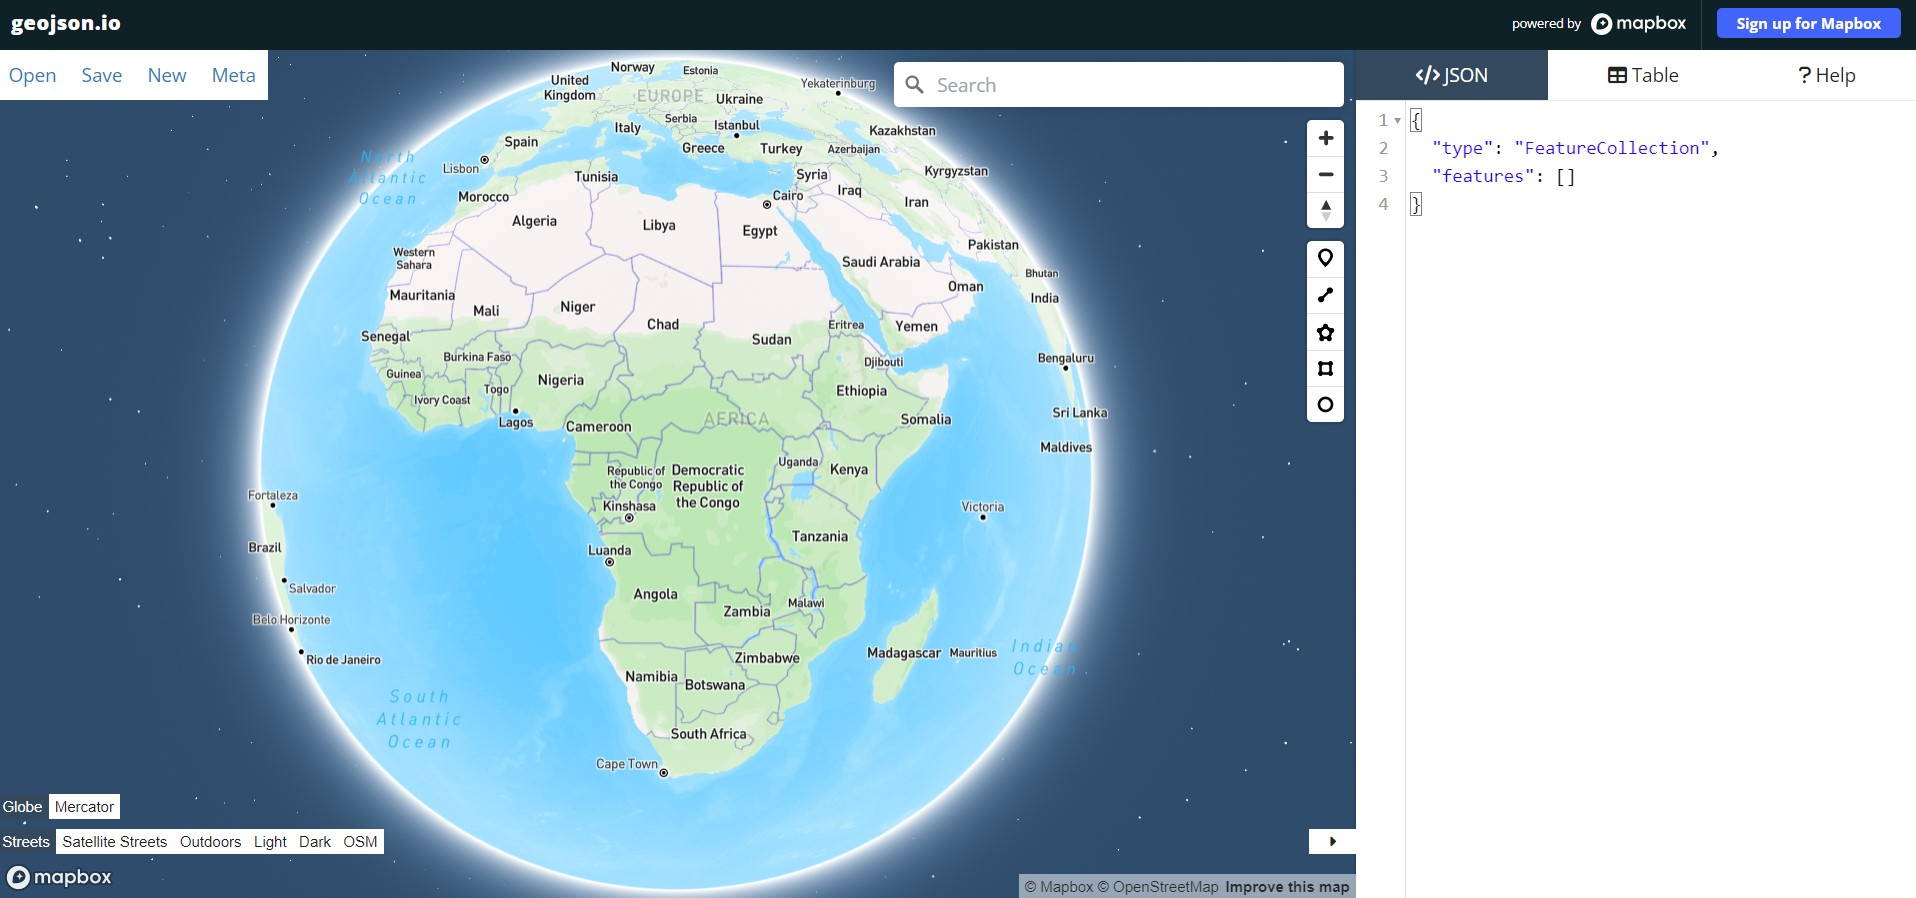
\includegraphics[width=26.61in]{../images/mapbox-front}

On your right, under the \textbf{\textless/\textgreater JSON} tab, the Mapbox folks have already given you a headstart by indicating what feature type and features will go into your \texttt{geojson} file. These are important as any website uses these keywords when parsing information from the GeoJSON file. Zoom to Kenya and click a point on top of the Nairobi dot pin, like shown below. Use the highlighted pin in the image below to create a marker over Nairobi.

\begin{Shaded}
\begin{Highlighting}[]
\NormalTok{knitr}\SpecialCharTok{::}\FunctionTok{include\_graphics}\NormalTok{(}\FunctionTok{rep}\NormalTok{(}\StringTok{"D:/gachuhi/my{-}leaflet/images/nairobi{-}pin.jpg"}\NormalTok{))}
\end{Highlighting}
\end{Shaded}

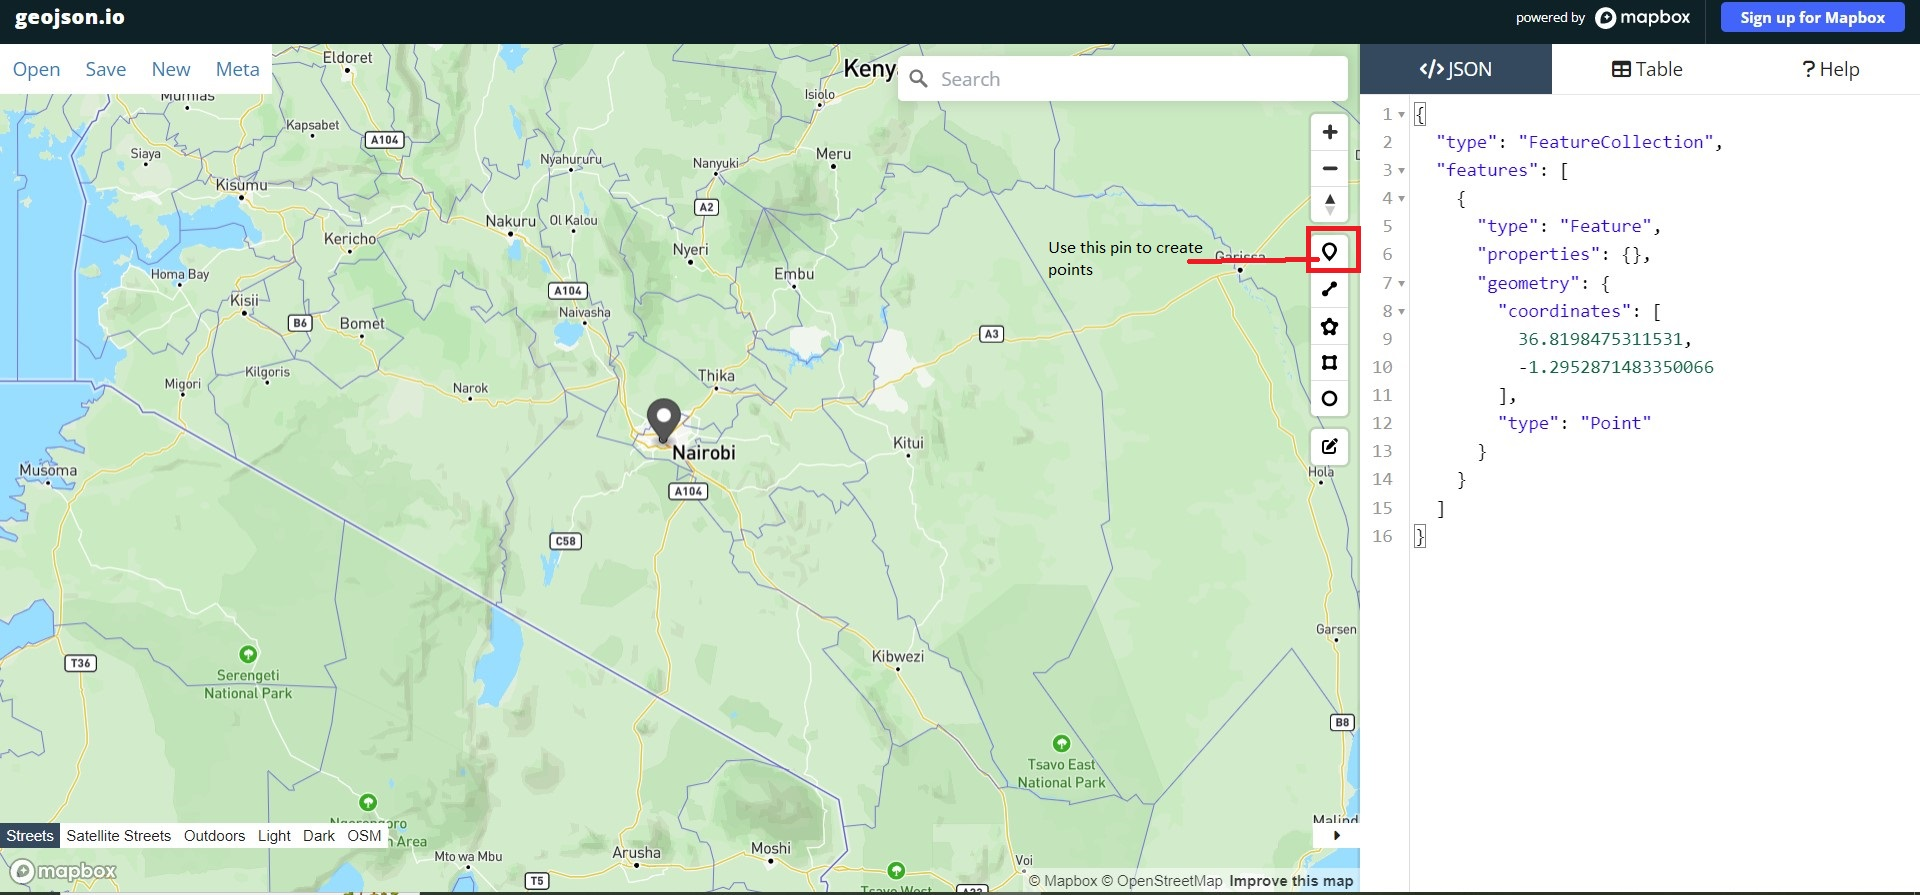
\includegraphics[width=26.67in]{../images/nairobi-pin}

By doing so, you will realize that a new dictionary of \texttt{type}, \texttt{properties} and \texttt{geometry} appears within the \textbf{features} list. These new keys provide the additional spatial and geometry data in their values in which a website when parsing this information can place them at their appropriate earth locations.

Now move over to the \textbf{Table} tab and click new column as shown below.

\begin{Shaded}
\begin{Highlighting}[]
\NormalTok{knitr}\SpecialCharTok{::}\FunctionTok{include\_graphics}\NormalTok{(}\FunctionTok{rep}\NormalTok{(}\StringTok{"D:/gachuhi/my{-}leaflet/images/table.jpg"}\NormalTok{))}
\end{Highlighting}
\end{Shaded}

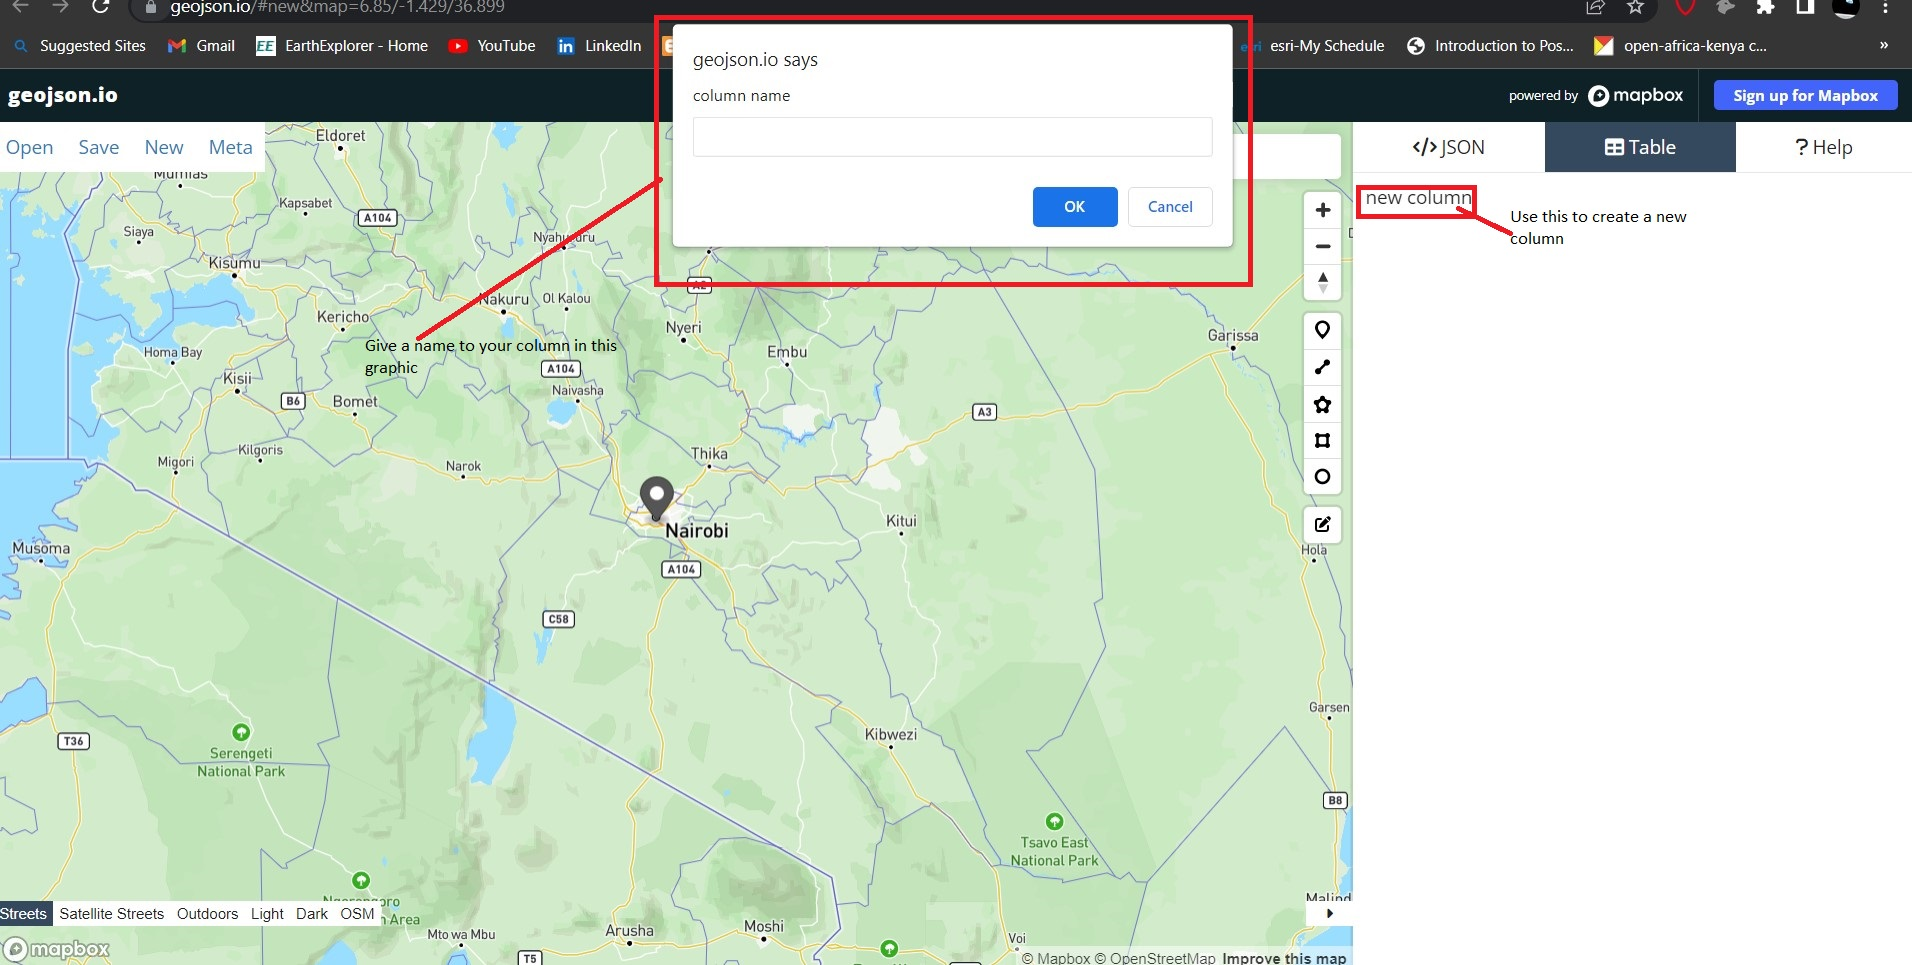
\includegraphics[width=26.56in]{../images/table}

Click on it and in the graphic that appears, give your column the name \textbf{City}. Click \textbf{Ok} and in the table cell that appears, type \textbf{Nairobi}.

\begin{Shaded}
\begin{Highlighting}[]
\NormalTok{knitr}\SpecialCharTok{::}\FunctionTok{include\_graphics}\NormalTok{(}\FunctionTok{rep}\NormalTok{(}\StringTok{"D:/gachuhi/my{-}leaflet/images/nairobi{-}named.jpg"}\NormalTok{))}
\end{Highlighting}
\end{Shaded}

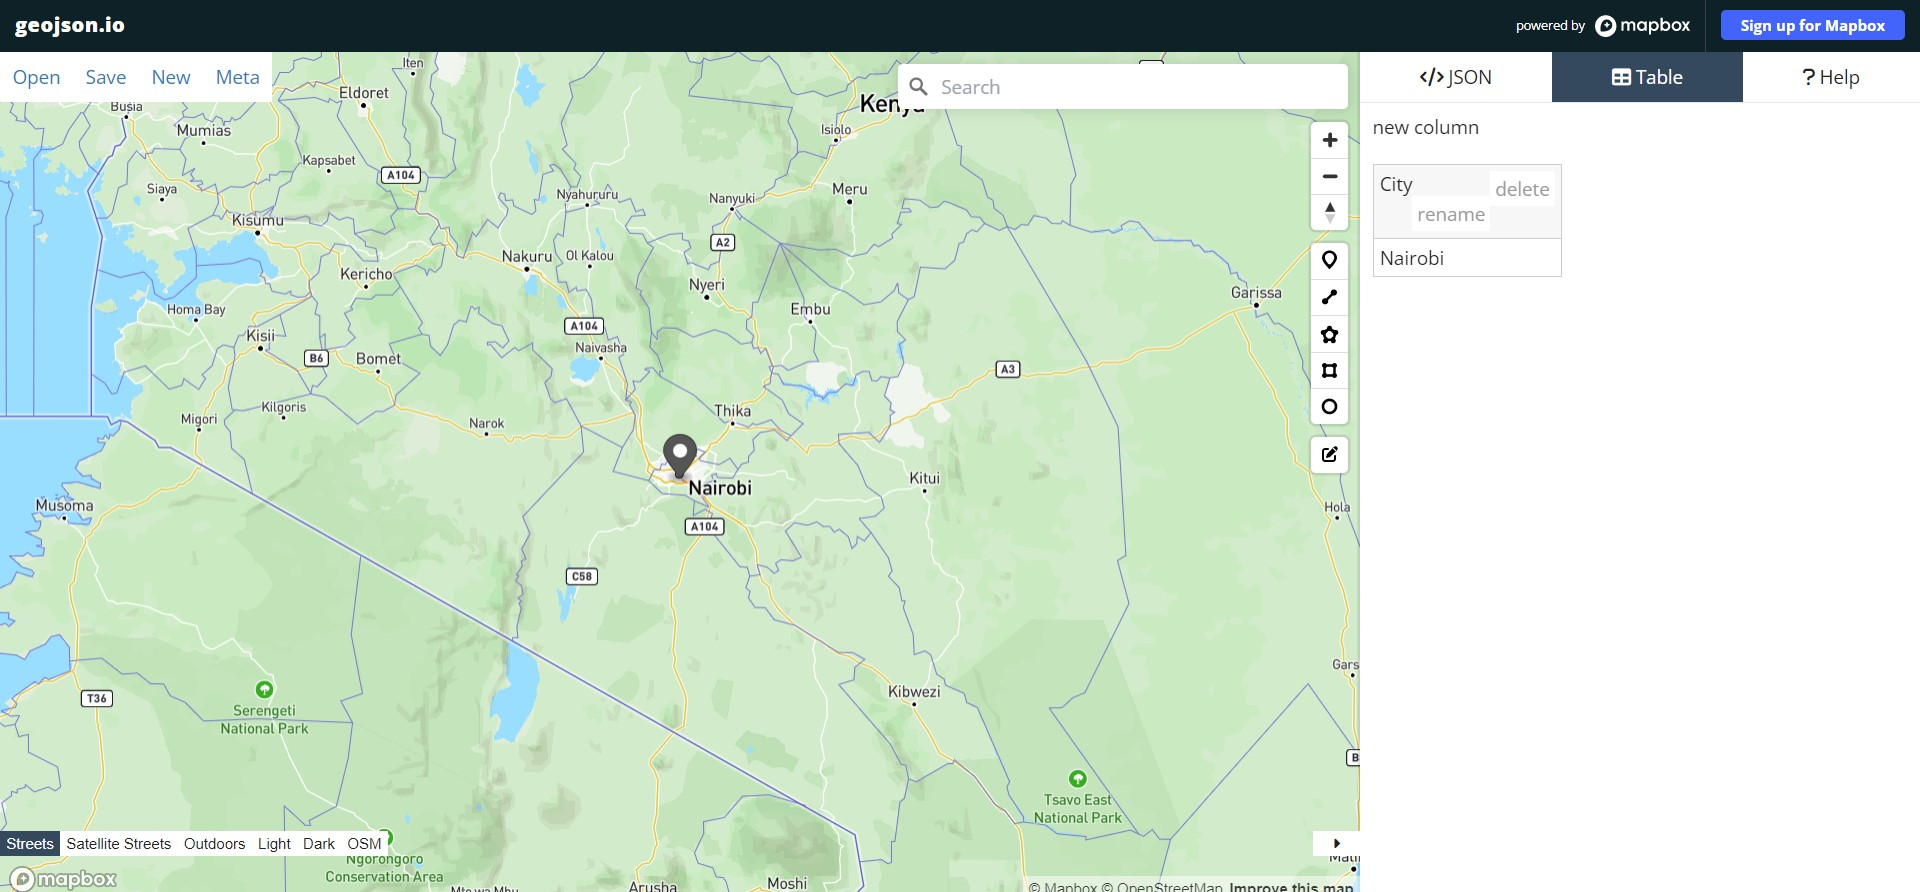
\includegraphics[width=26.67in]{../images/nairobi-named}

Now create a new pin over \emph{Kisumu} and a new dictionary will appear below that of Nairobi and a new table row will appear in the \textbf{Table} tab. Do the rest for the following cities: Mombasa, Nakuru, Nyeri, Machakos and Malindi. Legally speaking, only the first four are cities by law, the rest are just towns but for the sake of this tutorial, let's corporately refer to them as cities.

\begin{Shaded}
\begin{Highlighting}[]
\NormalTok{knitr}\SpecialCharTok{::}\FunctionTok{include\_graphics}\NormalTok{(}\FunctionTok{rep}\NormalTok{(}\StringTok{"D:/gachuhi/my{-}leaflet/images/cities{-}named.jpg"}\NormalTok{))}
\end{Highlighting}
\end{Shaded}

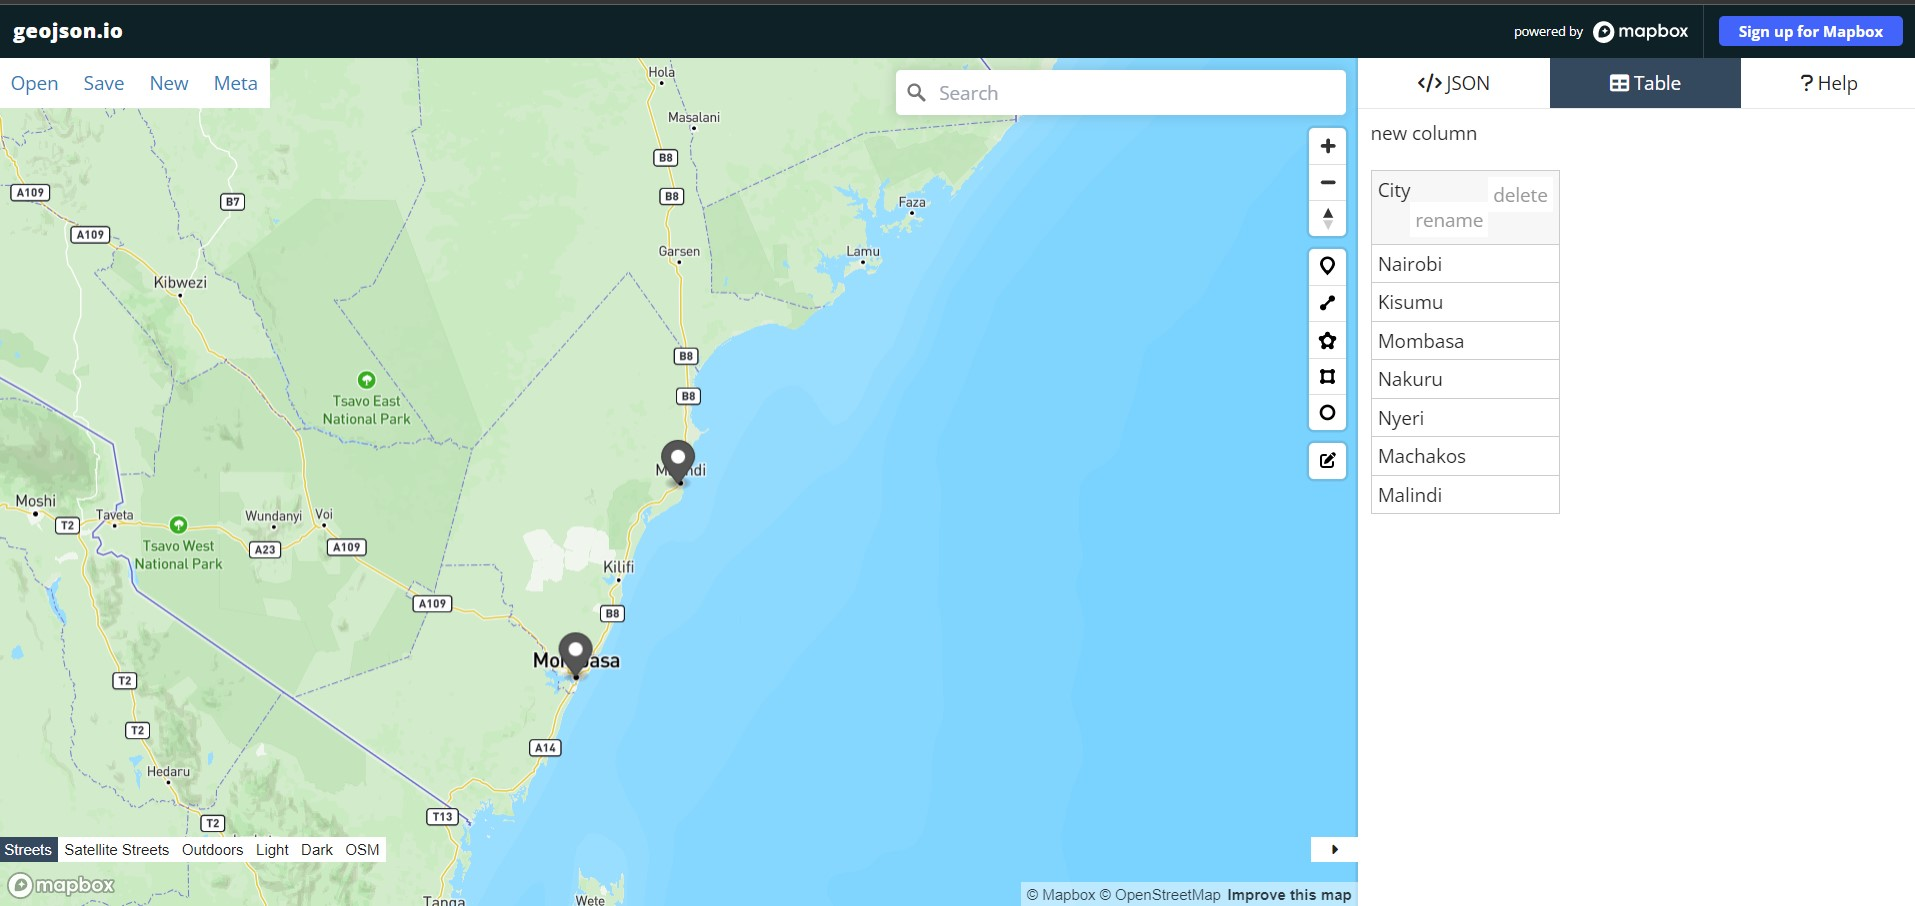
\includegraphics[width=26.6in]{../images/cities-named}

Alright, one process down, one more to go. We will fill these cities with their population statistics. Create a new column with the heading ``Population''. Fill each of the cities with the following statistics.

\begin{Shaded}
\begin{Highlighting}[]
\FunctionTok{read.csv}\NormalTok{(}\StringTok{"D:/gachuhi/my{-}leaflet{-}vs/data/points.csv"}\NormalTok{)[ , }\DecValTok{1}\SpecialCharTok{:}\DecValTok{2}\NormalTok{]}
\end{Highlighting}
\end{Shaded}

\begin{verbatim}
##       City  Population
## 1  Nairobi 4, 300, 000
## 2   Kisumu    610, 082
## 3  Mombasa 1, 440, 000
## 4   Nakuru    422, 000
## 5    Nyeri    759, 164
## 6 Machakos 1, 422, 000
## 7  Malindi    119, 859
\end{verbatim}

Once done, head over to the top left of the \href{http://geojson.io/}{geojson.io} website, and click \textbf{Save}. A list of options will appear, click on save as \textbf{geojson}. It should appear somewhere in your \emph{Downloads} directory.

\begin{Shaded}
\begin{Highlighting}[]
\NormalTok{knitr}\SpecialCharTok{::}\FunctionTok{include\_graphics}\NormalTok{(}\FunctionTok{rep}\NormalTok{(}\StringTok{"D:/gachuhi/my{-}leaflet/images/geojson{-}save.jpg"}\NormalTok{))}
\end{Highlighting}
\end{Shaded}

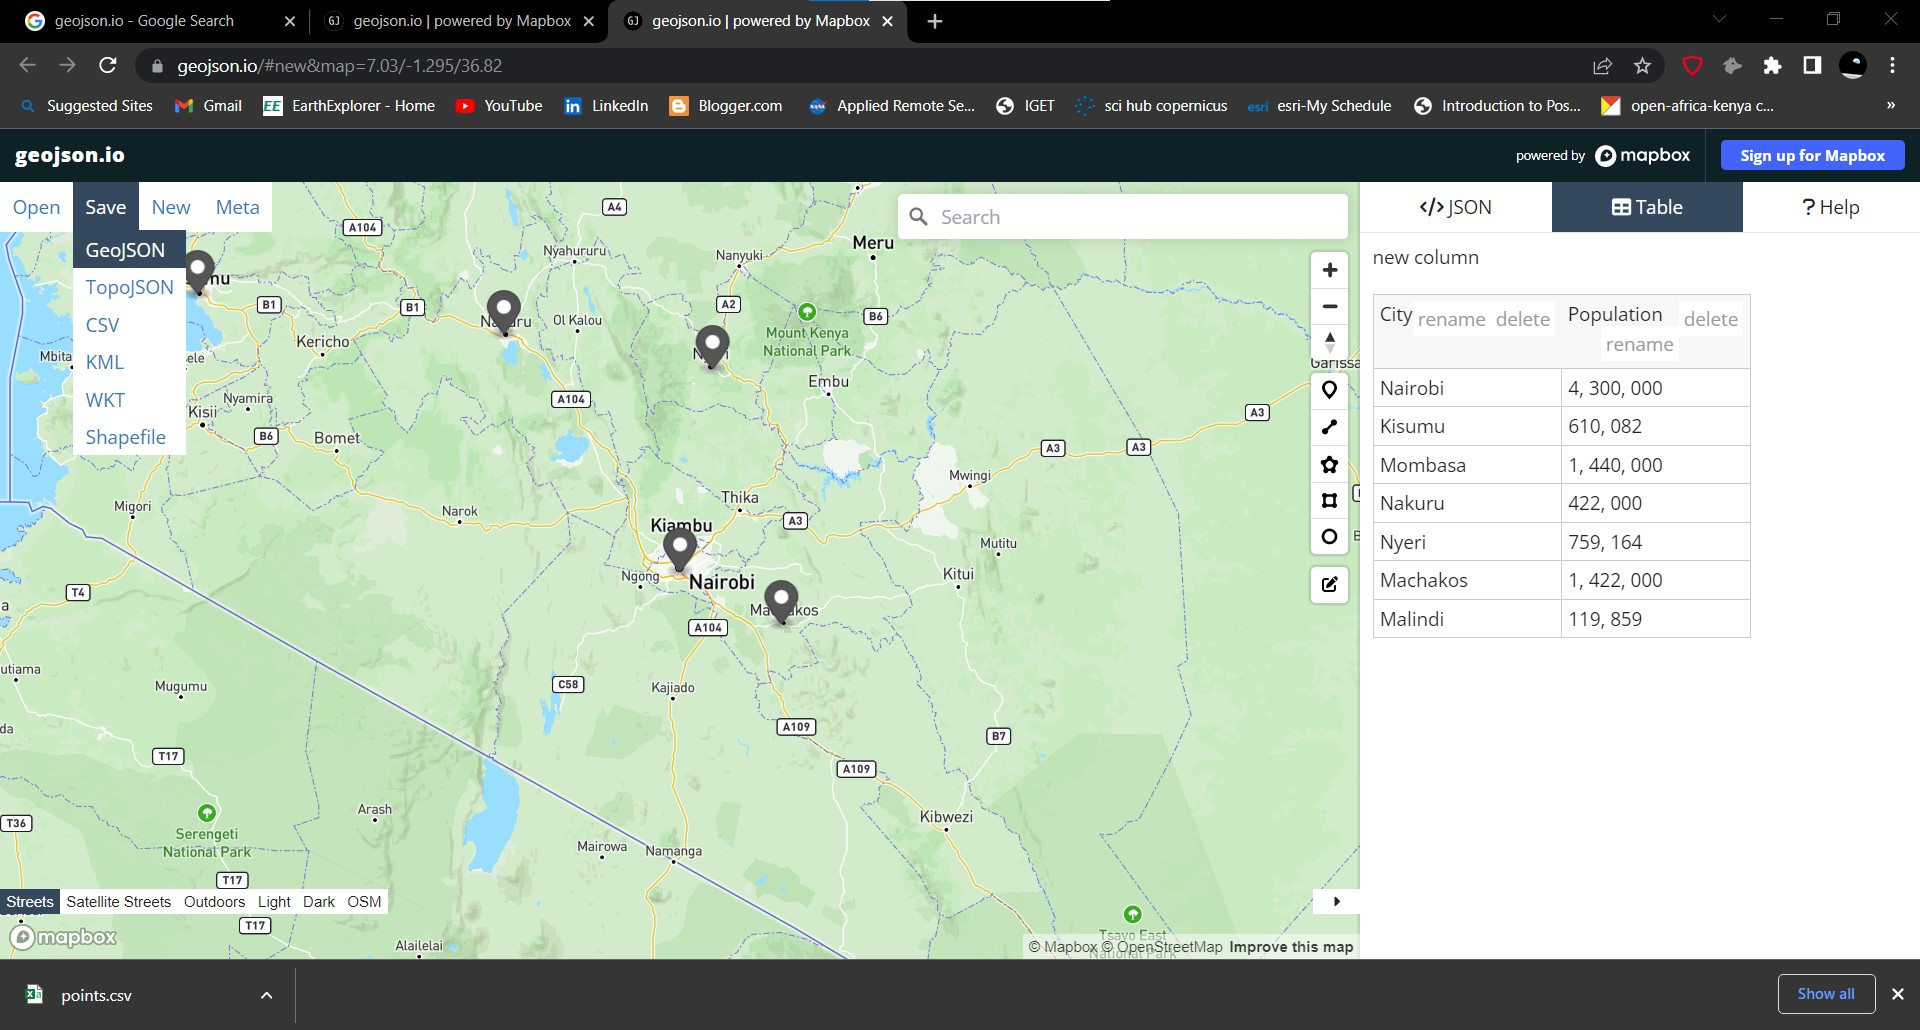
\includegraphics[width=26.67in]{../images/geojson-save}

\hypertarget{saving-the-geojson-to-github}{%
\section{Saving the Geojson to Github}\label{saving-the-geojson-to-github}}

Now, based on experience, using a local Geojson file (one within your computer directory) is painful in JavaScript. The error I faced had to do with servers or something. To get a way around this and still be able to display \texttt{.geojson} data in Leaflet, the data had to be stored on an online server, in this case Github. We would love to show you how to save data on Github, but this would make this chapter long. Therefore, and with sincere apologies, it would be best if you googled it out.

However, on the bright side, we have provided the GeoJSON we will use accessible from this \href{https://raw.githubusercontent.com/sammigachuhi/geojson_files/main/cities-geojson.geojson}{link}.

\hypertarget{loading-the-geojson-into-leaflet}{%
\section{Loading the GeoJSON into Leaflet}\label{loading-the-geojson-into-leaflet}}

As they always say, there are many ways of killing a rat. There are around three ways in which to load GeoJson data into leaflet, at least from our discovery. We shall start with the easiest and most unreliable to what we consider the best. Let start with the easy one, loading a \texttt{.geojson} file from within our Javascript file itself.

\hypertarget{the-easy-way}{%
\subsection{The easy way}\label{the-easy-way}}

First of all create a blank JavaScript file called \texttt{geojson.js}. Thereafter, go to your \texttt{map.html} file which you had created last in \protect\hyperlink{setting-the-superstructure}{Chapter 2} Open it. Change the value in the \texttt{src} attribute within the \texttt{\textless{}script\textgreater{}} tag of the \texttt{\textless{}body\textgreater{}}--the one inside the \texttt{\textless{}div\textgreater{}} element with \texttt{id="myMap"} to read \texttt{"geojson.io"} like below.

\begin{verbatim}
<!DOCTYPE html>
<html lang="en">
    <head>
        -- snip ---
    </head>
    <body>
        <div id="myMap">
            <script src="geojson.js">
            </script> 
        </div>  
        
    </body>
</html>
\end{verbatim}

Alright. Head over to your \texttt{geojson.js} and as always, add the leaflet classes \texttt{L.map} and \texttt{L.tileLayer}. We set the view of our new Leaflet map to that of Nairobi. Your blank \texttt{geojson.js} should now be filled with the below code.

\begin{verbatim}
var map = L.map('myMap').setView([-1.295287148, 36.81984753], 7);

L.tileLayer('https://tile.openstreetmap.org/{z}/{x}/{y}.png', {
    maxZoom: 19,
    attribution: '&copy; <a href="http://www.openstreetmap.org/copyright">OpenStreetMap</a>'
}).addTo(map);
\end{verbatim}

Okay. Head over to \url{geojson.io} website and right under the \textbf{\textless/\textgreater JSON} you will see a copy icon.

\begin{Shaded}
\begin{Highlighting}[]
\NormalTok{knitr}\SpecialCharTok{::}\FunctionTok{include\_graphics}\NormalTok{(}\FunctionTok{rep}\NormalTok{(}\StringTok{"D:/gachuhi/my{-}leaflet/images/geojson{-}copy.jpg"}\NormalTok{))}
\end{Highlighting}
\end{Shaded}

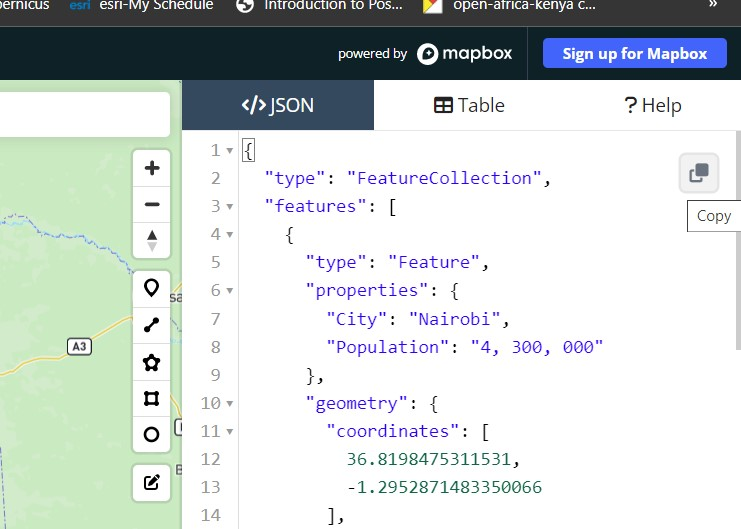
\includegraphics[width=10.29in]{../images/geojson-copy}
Click it and past it in your \texttt{geojson.js} file right above the other \texttt{L.map} and \texttt{L.tileLayer} classes. Your \texttt{geojson.js} should look like below.

\begin{verbatim}
var cities = {
    "type": "FeatureCollection",
    "features": [
      {
        "type": "Feature",
        "properties": {
          "City": "Nairobi",
          "Population": "4, 300, 000"
        },
        "geometry": {
          "coordinates": [
            36.8198475311531,
            -1.2952871483350066
          ],
          "type": "Point"
        }
      },
      -- snip ---
      {
        "type": "Feature",
        "properties": {
          "City": "Malindi",
          "Population": "119, 859"
        },
        "geometry": {
          "coordinates": [
            40.10521499751357,
            -3.2138767356491655
          ],
          "type": "Point"
        }
      }
    ]
  }


var map = L.map('myMap').setView([-1.295287148, 36.81984753], 7);

L.tileLayer('https://tile.openstreetmap.org/{z}/{x}/{y}.png', {
    maxZoom: 19,
    attribution: '&copy; <a href="http://www.openstreetmap.org/copyright">OpenStreetMap</a>'
}).addTo(map);
\end{verbatim}

Refresh your \texttt{map.html}. It's a map of Kenya alright, but none of our \texttt{.geojson} features appear yet. We are about to change that. Leaflet offers the \texttt{L.geoJSON} class to add GeoJSON data to a map. The class speaks for itself therefore, let's use it to add our GeoJSON features. Add the following code below the other leaflet map class layers.

\begin{verbatim}
L.geoJSON(cities).addTo(map);
\end{verbatim}

Refresh your \texttt{map.html}. The GeoJSON features should now appear at their exact locations.

\begin{Shaded}
\begin{Highlighting}[]
\NormalTok{knitr}\SpecialCharTok{::}\FunctionTok{include\_graphics}\NormalTok{(}\FunctionTok{rep}\NormalTok{(}\StringTok{"D:/gachuhi/my{-}leaflet/images/geojson{-}leaflet.jpg"}\NormalTok{))}
\end{Highlighting}
\end{Shaded}

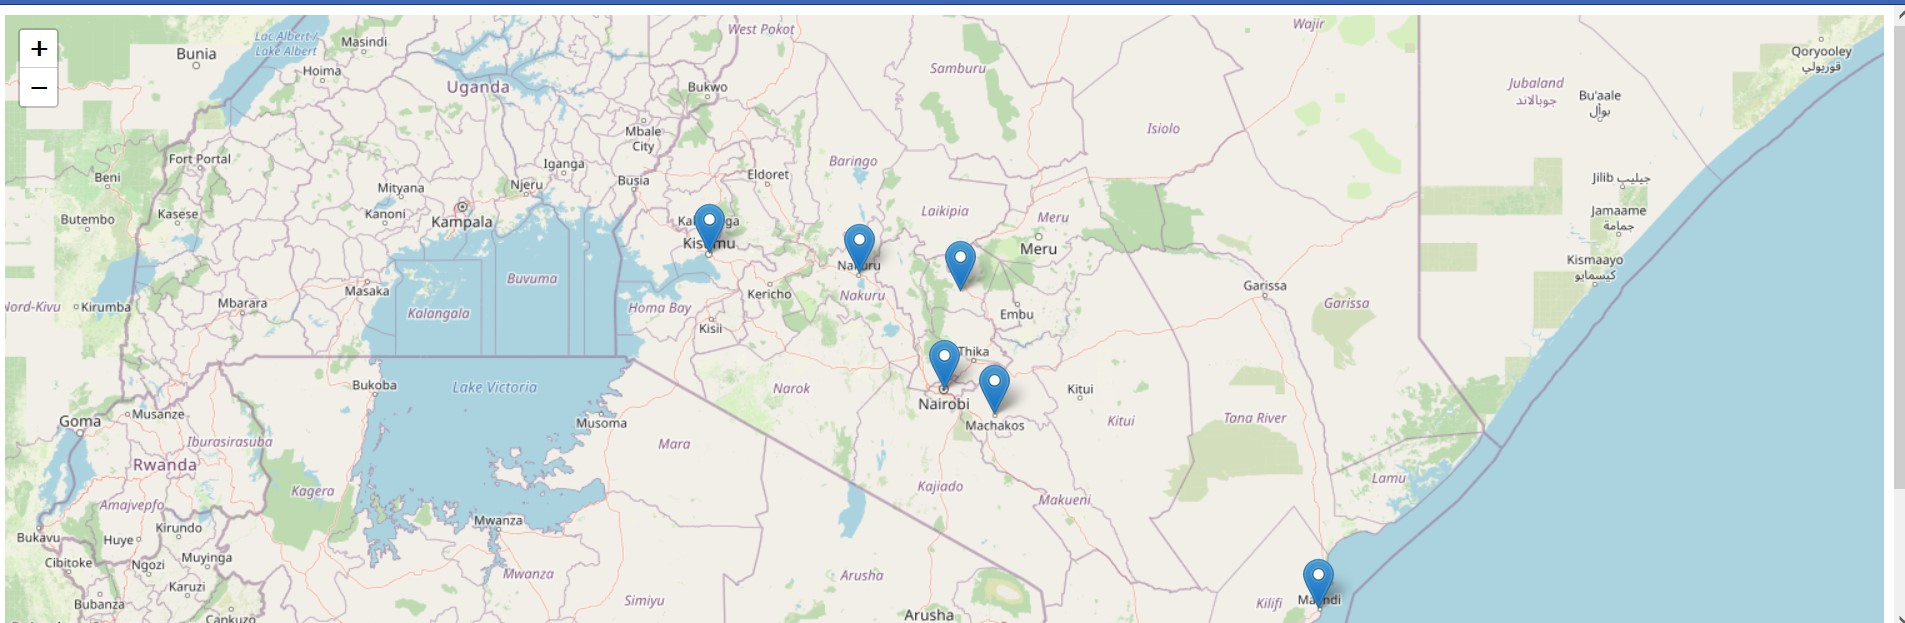
\includegraphics[width=26.46in]{../images/geojson-leaflet}

How about if we made the markers more interactive, say they display popups as we did in \protect\hyperlink{a-marker-with-a-popup}{Chapter 3}? We want the city names to appear when the user clicks on the markers. Easy. Just create a function that does so as in the logic provided \href{https://leafletjs.com/reference.html\#geojson}{here}. We customized it to our case to make sure it references to the \texttt{City} key which is part of the dictionary attached to the \texttt{properties} key.

\begin{verbatim}
L.geoJSON(cities).bindPopup(function (layer) {
    return layer.feature.properties.City;
}).addTo(map);
\end{verbatim}

\begin{Shaded}
\begin{Highlighting}[]
\NormalTok{knitr}\SpecialCharTok{::}\FunctionTok{include\_graphics}\NormalTok{(}\FunctionTok{rep}\NormalTok{(}\StringTok{"D:/gachuhi/my{-}leaflet/images/geojson{-}names.jpg"}\NormalTok{))}
\end{Highlighting}
\end{Shaded}

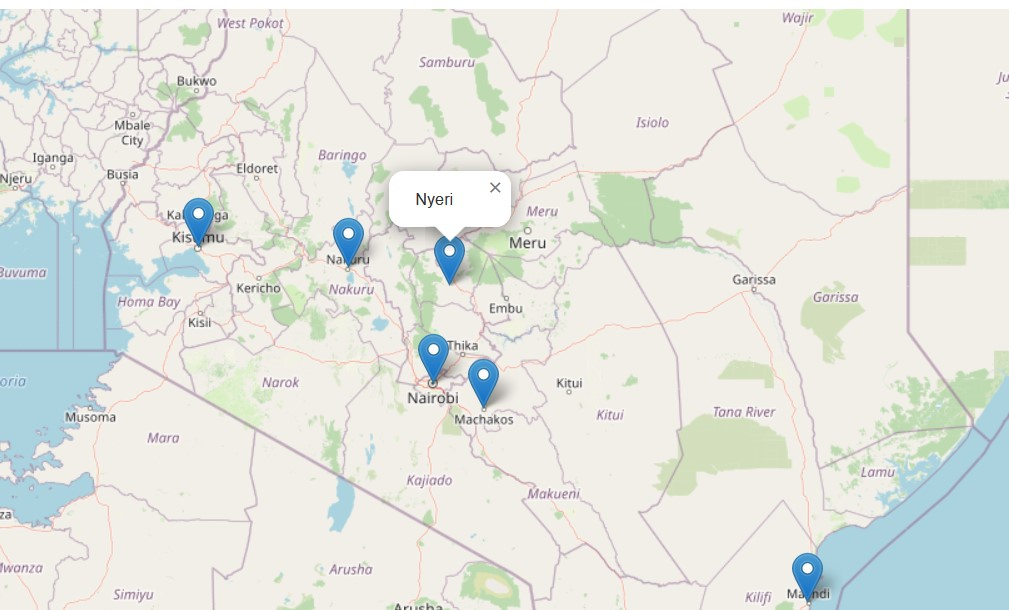
\includegraphics[width=14.01in]{../images/geojson-names}

There is one issue with this method. If we have a very long GeoJSON data structure, it will clatter our JavaScript file. We only worked with seven cities, but it is very common to work with data holding hundreds and even thousands of dictionaries. That would make your JavaScript file stretch to \emph{ad infitum}.

This brings us to the other two methods, that of using the \textbf{Ajax} plugin and using the \textbf{Fetch} Application Programming Interface (API). Don't let the words scare you. Take a break, grab a glass of water and come back.

\hypertarget{using-the-ajax-plugin}{%
\subsection{Using the Ajax Plugin}\label{using-the-ajax-plugin}}

As the term `plugin' suggests, this is an extension that offers additional functions to the core Leaflet plugin. The Ajax plugin is available from this \href{https://github.com/calvinmetcalf/leaflet-ajax/archive/refs/heads/gh-pages.zip}{link}. Download it to your directory preferably within the same directory as your \texttt{map.html} and \texttt{geojson.js}. Alright. Right under the \texttt{src} for \texttt{leaflet.js} in your \texttt{map.html}. Add the following \texttt{\textless{}script\textgreater{}} tag.

\begin{verbatim}
    <head>
        -- snip --
        <script src="leaflet-ajax-gh-pages\dist\leaflet.ajax.js"></script>
        
    </head>
    -- snip --
\end{verbatim}

This file will allow you to add \texttt{.geojson} files to your Leaflet map. However, there is a catch, both the Ajax and Fetch APIs only work with GeoJson file formats saved on a web server. Based on experience, they will not work with local GeoJson files. As a work around, we saved our GeoJSON file to Github. Don't worry, here is the \href{https://raw.githubusercontent.com/sammigachuhi/geojson_files/main/cities-geojson.geojson}{link} to the raw \texttt{.geojson} file we had created earlier.

We shall call our GeoJSON file from Github using Ajax as shown in the code below. Please remember to comment out your \texttt{var\ cities} and \texttt{L.geoJSON} using \texttt{\textbackslash{}\textbackslash{}} because they are irrelevant in this particular case. You actually should.

\begin{verbatim}
var geojsonLayer = new L.geoJson.ajax("https://raw.githubusercontent.com/sammigachuhi/geojson_files/main/cities-geojson.geojson").addTo(map);
\end{verbatim}

Your map should now show the markers of our cities. If you are hawk eyed, you may have noticed that the syntax is a bit different, both from the Ajax Website and that of the \texttt{L.geoJSON} from Leaflet. Starting with the latter, we have instead used \texttt{L.geoJson} and unlike in the creators website where he used \texttt{var\ geojsonLayer\ =\ new\ L.GeoJSON.AJAX(\textless{}your-geojson-file\textgreater{})} we used the following syntax: \texttt{L.geoJson.ajax()} (ajax and geoJson begin with small case). Actually, that's what worked after a lengthy web search.

Just like using \texttt{L.geoJSON}, we can also add popups after calling the \texttt{.ajax} method.

\begin{verbatim}
var geojsonLayer = new L.geoJson.ajax("https://raw.githubusercontent.com/sammigachuhi/geojson_files/main/cities-geojson.geojson")
    .bindPopup(function (layer) {
        return layer.feature.properties.City;
    }).addTo(map);
\end{verbatim}

Doing so should make the city names appear on click on your leaflet map.

\hypertarget{using-fetch-api}{%
\subsection{Using Fetch API}\label{using-fetch-api}}

Fetch API is a modern interface that allows you to make HTTP requests to servers from web browsers. In other words, it searches for a resource over the web and retrieves it, thus giving it back to you. Think of it as a dog in which you throw a saucer and tell your faithful hound ``Sabre, fetch!''. The dog runs after the saucer, grips it with its canines before it touches ground and quickly brings it back to you. Same case with Fetch API!

We had mentioned we will show how to retreive our Github stored GeoJSON data and we shall stick to the script. We shall also attempt to explain how this \texttt{fetch} works.

First things first. We shall call the \texttt{fetch} function and pass it our Github url containing our GeoJSON text. Since \texttt{fetch} is an API, it retrieves data from Github.io --the server in this case--and brings it to our laptop the -- the client. Enough IT. Let's write it down.

\begin{verbatim}
fetch("https://raw.githubusercontent.com/sammigachuhi/geojson_files/main/cities-geojson.geojson")
\end{verbatim}

Okay. Next step, once the server beams back the data to us, what do we do with it? According to \href{https://www.digitalocean.com/community/tutorials/js-fetch-api}{Digital Ocean}, the response is not \emph{actually} the data in the original format but rather \emph{a series of methods that can be used depending on what you want to do with the information}. We have to convert the object to a specific format. In this case, a JSON format. And to do this data conversion, the \texttt{json()} method is used. Actually, a function is created to do this. In the code below the function appears in parenthesis after \texttt{.then}.

\begin{verbatim}
fetch("https://raw.githubusercontent.com/sammigachuhi/geojson_files/main/cities-geojson.geojson")
    .then(function(response) {
        return response.json()
    })
\end{verbatim}

The above function takes the \texttt{response} argument and convert it to JSON by appending the \texttt{.json()} method to it.

After converting our response to JSON, it still needs to be processed further. Processed to what? To a GeoJSON file and subsequently add it to our Leaflet Map.

\begin{verbatim}
fetch("https://raw.githubusercontent.com/sammigachuhi/geojson_files/main/cities-geojson.geojson")
    .then(function(response) {
        return response.json()
    })
    .then(function(data) {
        L.geoJson(data).addTo(map);
    })
\end{verbatim}

We shall also add one more function --the \texttt{catch()} method. \texttt{catch()} is a method that returns an action if our response to the server has been rejected. We shall show the code and demonstrate it.

\begin{verbatim}
fetch("https://raw.githubusercontent.com/sammigachuhi/geojson_files/main/cities-geojson.geojson")
    .then(function(response) {
        return response.json()
    })
    .then(function(data) {
        L.geoJson(data).addTo(map);
    })
    .catch(function(error) {
        console.log(`This is the error: ${error}`)
    })
\end{verbatim}

To see the \texttt{catch()} in action, omit the last letter in our url so that it reads \texttt{cities-geojson.geojso}. You read it right. Just omit the letter `n' for now for goodness sake. Reload your \texttt{map.html}. Right click the webmap page and click on \textbf{Inspect} in the small interface that appears. Head over to the console tab and see the error response. It should read like below.

\begin{Shaded}
\begin{Highlighting}[]
\NormalTok{knitr}\SpecialCharTok{::}\FunctionTok{include\_graphics}\NormalTok{(}\FunctionTok{rep}\NormalTok{(}\StringTok{"D:/gachuhi/my{-}leaflet/images/catch{-}error.jpg"}\NormalTok{))}
\end{Highlighting}
\end{Shaded}

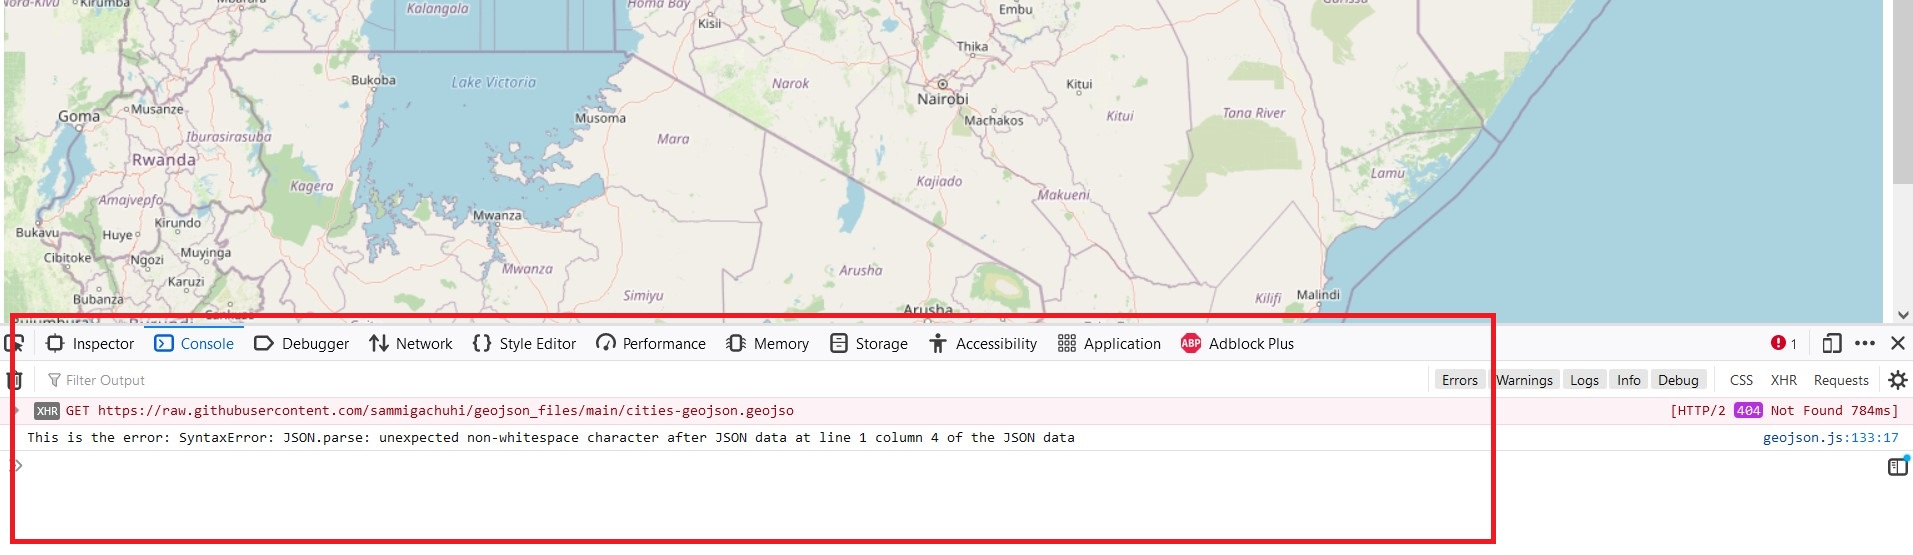
\includegraphics[width=26.57in]{../images/catch-error}

Restore the omitted letter and reload your \texttt{map.html}. Your leaflet map should have the city markers overlain just like in the case of using Ajax plugin or hardcoding the Geojson data into \texttt{var\ cities}. To stretch your Javascript skills further, we can shorten our code further by retaining the arguments \texttt{response}, \texttt{data} and \texttt{error} and using the arrow function \texttt{=\textgreater{}} to pass on the return statements, like so.

\begin{verbatim}
fetch("https://raw.githubusercontent.com/sammigachuhi/geojson_files/main/cities-geojson.geojson")
    .then((response) =>{
        return response.json()
    })
    .then((data) => {
        L.geoJson(data).addTo(map);
    })
    .catch((error) => {
        console.log(`This is the error: ${error}`)
    })
\end{verbatim}

It looks cryptic but don't cry! We have only ommitted the \texttt{function()} keyword and instead added \texttt{=\textgreater{}} between \texttt{function()} and the curly brackets \texttt{\{\textless{}code-to-run\textgreater{}\}} which is the function body, aka where the magic happens. Just like when using Ajax, we can also add other functionalities within \texttt{L.geoJSON}. In here, and thanks to the use of template literals \texttt{(\textasciigrave{}\textasciigrave{})}, we can even add statements and refer to our GeoJson keys (and in some cases, even variables) using \texttt{\$\{\}}. Whatever is within the \texttt{\$\{\}} is executed and passed out as a string to the template literals.

\begin{verbatim}
fetch("https://raw.githubusercontent.com/sammigachuhi/geojson_files/main/cities-geojson.geojson")
    .then((response) =>{
        return response.json()
    })
    .then((data) => {
        L.geoJson(data).bindPopup((layer) => {
            return `City: ${layer.feature.properties.City},<br>
            Population: ${layer.feature.properties.Population}`}).addTo(map);
    })
    .catch((error) => {
        console.log(`This is the error: ${error}`)
    })
\end{verbatim}

In our case, we added the HTML tag \texttt{\textless{}br\textgreater{}} to separate the \texttt{City} and \texttt{Population} keys from our GeoJSON. What we have are neat markers showing both the city name and population figures in two separate lines.

Phew! Enough Javascript for a day!

\begin{Shaded}
\begin{Highlighting}[]
\NormalTok{knitr}\SpecialCharTok{::}\FunctionTok{include\_graphics}\NormalTok{(}\FunctionTok{rep}\NormalTok{(}\StringTok{"D:/gachuhi/my{-}leaflet/images/city{-}population.jpg"}\NormalTok{))}
\end{Highlighting}
\end{Shaded}

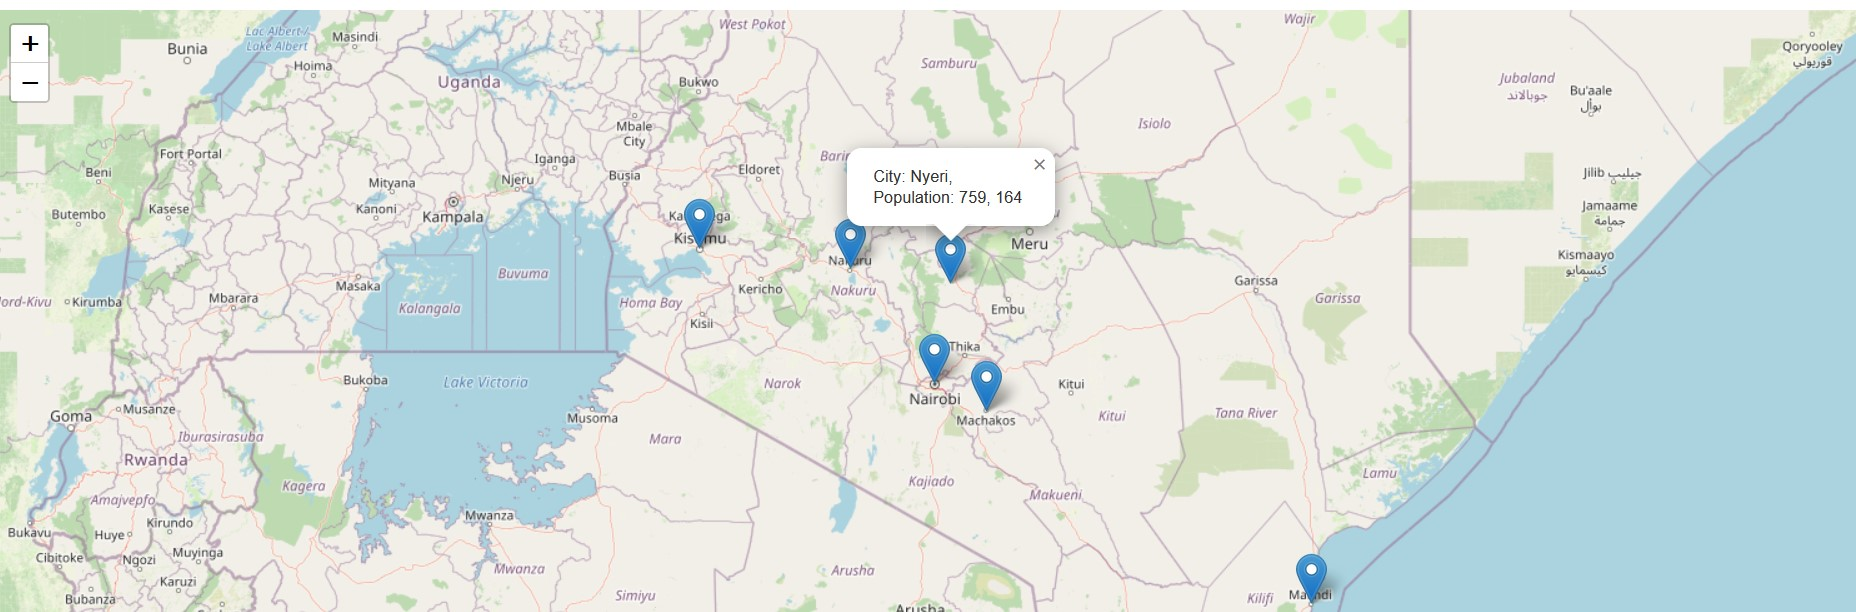
\includegraphics[width=25.78in]{../images/city-population}

Here are the \href{https://www.dropbox.com/scl/fo/uj45qo0gmed5xudmw1xja/h?dl=0\&rlkey=09mhhfdualbs92f7wg5atgdrx}{full files}.

\hypertarget{create-your-own-custom-markers}{%
\chapter{Create your own custom markers}\label{create-your-own-custom-markers}}

Full codes and files are \href{https://www.dropbox.com/scl/fo/ecidt41insvnzpwvmj9iw/h?dl=0\&rlkey=yy4w9p76osxs913p19wvnsjez}{here}.

Hope you didn't trash away the cities we created in the last \protect\hyperlink{using-geojson-in-leaflet}{chapter}. In this chapter, we shall focus on creating your own custom markers. We love a clean job, so we will create a new JavaScript file and name it \texttt{custom-markers.js}. We understand the previous \protect\hyperlink{using-geojson-in-leaflet}{chapter} was quite long but believe you me, although creating custom markers sounds easier, it took us way longer to get the hang around it. Sounds ironic but its the truth. Good news, we received enough punches on the face to teach you how to dodge the pain points.

The very first thing is to create a basemap.

\begin{verbatim}
var map = L.map('myMap').setView([-1.295287148, 36.81984753], 7);

L.tileLayer('https://tile.openstreetmap.org/{z}/{x}/{y}.png', {
    maxZoom: 19,
    attribution: '&copy; <a href="http://www.openstreetmap.org/copyright">OpenStreetMap</a>'
}).addTo(map);
\end{verbatim}

We will create a new variable called \texttt{cities} that mimics the geojson file saved to github only these time the population values have been tweaked a bit. Paste the below code to your \texttt{custom-markers.js}.

\begin{verbatim}
var cities = {
    "type": "FeatureCollection",
    "features": [
      {
        "type": "Feature",
        "properties": {
          "City": "Nairobi",
          "Population": 4300000
        },
        "geometry": {
          "coordinates": [
            36.8198475311531,
            -1.2952871483350066
          ],
          "type": "Point"
        }
      },
      {
        "type": "Feature",
        "properties": {
          "City": "Kisumu",
          "Population": 610082
        },
        "geometry": {
          "coordinates": [
            34.74657469430895,
            -0.10402992528247523
          ],
          "type": "Point"
        }
      },
      {
        "type": "Feature",
        "properties": {
          "City": "Mombasa",
          "Population": 1440000
        },
        "geometry": {
          "coordinates": [
            39.66358575335434,
            -4.041883912902392
          ],
          "type": "Point"
        }
      },
      {
        "type": "Feature",
        "properties": {
          "City": "Nakuru",
          "Population": 422000
        },
        "geometry": {
          "coordinates": [
            36.06412271026528,
            -0.2754534004690896
          ],
          "type": "Point"
        }
      },
      {
        "type": "Feature",
        "properties": {
          "City": "Nyeri",
          "Population": 759164
        },
        "geometry": {
          "coordinates": [
            36.957036675396154,
            -0.42345404217887506
          ],
          "type": "Point"
        }
      },
      {
        "type": "Feature",
        "properties": {
          "City": "Machakos",
          "Population": 1422000
        },
        "geometry": {
          "coordinates": [
            37.25780808801821,
            -1.518874011494134
          ],
          "type": "Point"
        }
      },
      {
        "type": "Feature",
        "properties": {
          "City": "Malindi",
          "Population": 119859
        },
        "geometry": {
          "coordinates": [
            40.10521499751357,
            -3.2138767356491655
          ],
          "type": "Point"
        }
      }
    ]
  }
\end{verbatim}

Can you notice any difference on the \texttt{Population} property compared to the code \protect\hyperlink{using-geojson-in-leaflet}{Chapter 5}? If you are hawkeyed, you will see the Population values this time round are integers compared to strings in the previous chapter. It sounds superflous to create population values as strings only to convert them to integers now, but please do remember the geojson.io site did that for us, not this author. Here is the \href{https://raw.githubusercontent.com/sammigachuhi/geojson_files/main/cities-geojson2.geojson.txt}{raw geojson script} customized for this chapter.

Just a small note before going on. When the GeoJSON file has the population values enclosed in strings \texttt{""}, they are automatically rendered on a map on the Github server.

\begin{Shaded}
\begin{Highlighting}[]
\NormalTok{knitr}\SpecialCharTok{::}\FunctionTok{include\_graphics}\NormalTok{(}\FunctionTok{rep}\NormalTok{(}\StringTok{"D:/gachuhi/my{-}leaflet/images/geojson{-}webmap.jpg"}\NormalTok{))}
\end{Highlighting}
\end{Shaded}

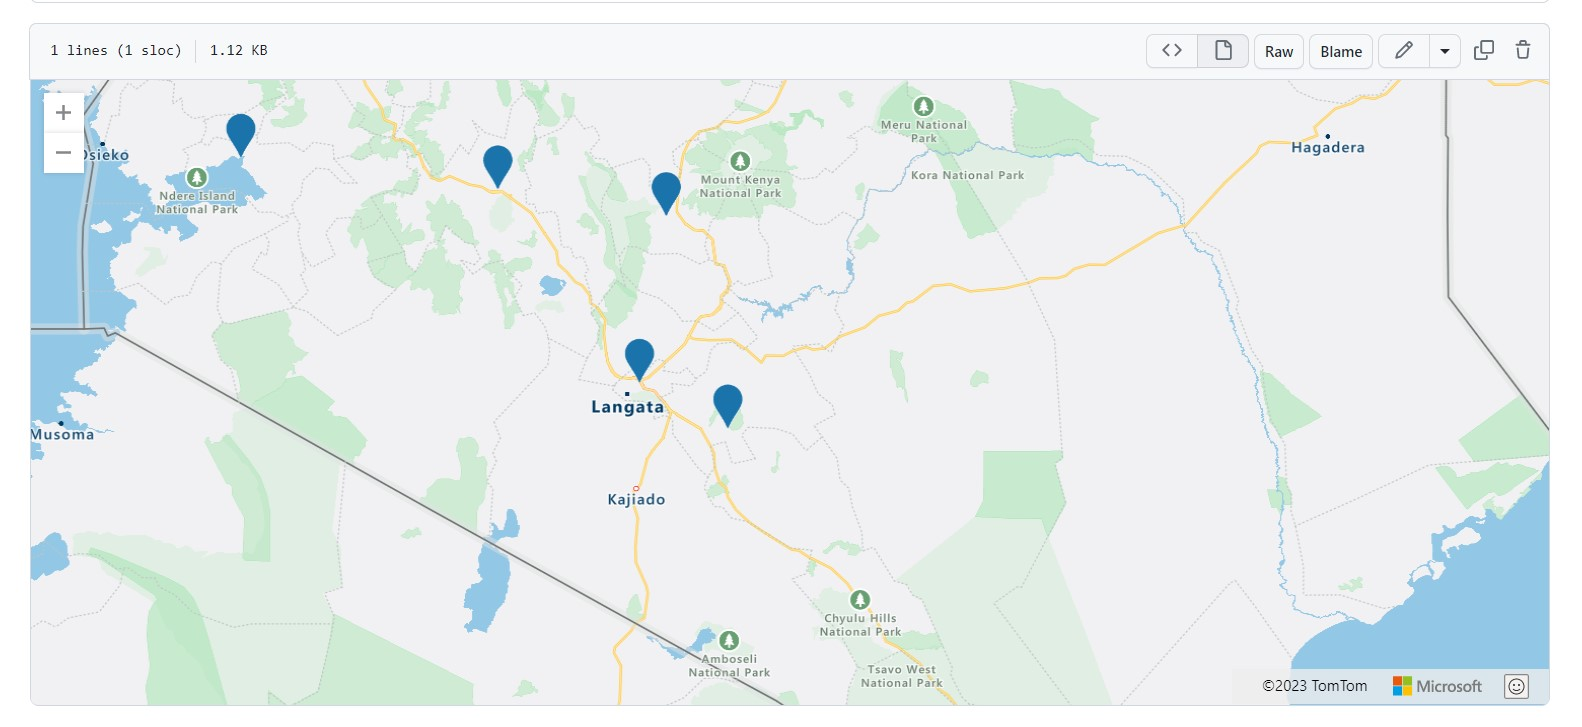
\includegraphics[width=21.97in]{../images/geojson-webmap}

However, when the strings are removed, and the population values remain as integers, they are no longer rendered on a webmap as shown below.

\begin{Shaded}
\begin{Highlighting}[]
\NormalTok{knitr}\SpecialCharTok{::}\FunctionTok{include\_graphics}\NormalTok{(}\FunctionTok{rep}\NormalTok{(}\StringTok{"D:/gachuhi/my{-}leaflet/images/geojson{-}nowebmap.jpg"}\NormalTok{))}
\end{Highlighting}
\end{Shaded}

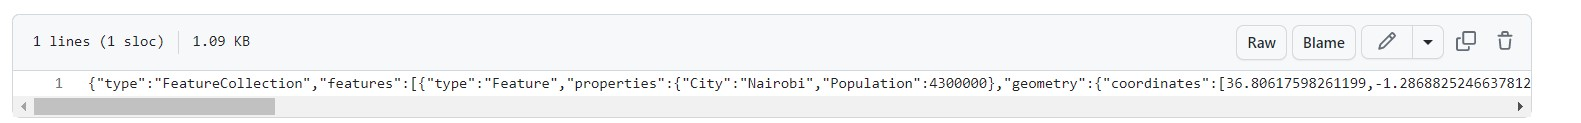
\includegraphics[width=21.96in]{../images/geojson-nowebmap}

It's just a dictionary of lists and other dictionaries.

\hypertarget{the-icons}{%
\section{The icons}\label{the-icons}}

Alright. Let's create a map of our cities but with custom markers this time round. The below code creates our custom markers.

\begin{verbatim}
// Yellow Icon
var yellowIcon = new L.Icon({
    iconUrl: 'https://raw.githubusercontent.com/pointhi/leaflet-color-markers/master/img/marker-icon-2x-yellow.png',
    shadowUrl: 'https://cdnjs.cloudflare.com/ajax/libs/leaflet/0.7.7/images/marker-shadow.png',
    iconSize: [25, 41],
    iconAnchor: [12, 41],
    popupAnchor: [1, -34],
    shadowSize: [41, 41]
  });

// Orange Icon
var orangeIcon = new L.Icon({
    iconUrl: 'https://raw.githubusercontent.com/pointhi/leaflet-color-markers/master/img/marker-icon-2x-orange.png',
    shadowUrl: 'https://cdnjs.cloudflare.com/ajax/libs/leaflet/0.7.7/images/marker-shadow.png',
    iconSize: [25, 41],
    iconAnchor: [12, 41],
    popupAnchor: [1, -34],
    shadowSize: [41, 41]
  });

// Red Icon
var redIcon = new L.Icon({
    iconUrl: 'https://raw.githubusercontent.com/pointhi/leaflet-color-markers/master/img/marker-icon-2x-red.png',
    shadowUrl: 'https://cdnjs.cloudflare.com/ajax/libs/leaflet/0.7.7/images/marker-shadow.png',
    iconSize: [25, 41],
    iconAnchor: [12, 41],
    popupAnchor: [1, -34],
    shadowSize: [41, 41]
  });
\end{verbatim}

We created three markers in order of importance. One is yellow, the other orange, the other red. You will see the significance (not so much) of these colors later.

Time to create GeoJSON markers out of this.

\begin{verbatim}
L.geoJSON(cities, {
    pointToLayer(feature, latlng) {
        return L.marker(latlng, {icon: yellowIcon});
    }
}).bindPopup(function (layer) {
    return layer.feature.properties.City;
}).addTo(map);
\end{verbatim}

We got this.

\begin{Shaded}
\begin{Highlighting}[]
\NormalTok{knitr}\SpecialCharTok{::}\FunctionTok{include\_graphics}\NormalTok{(}\FunctionTok{rep}\NormalTok{(}\StringTok{"D:/gachuhi/my{-}leaflet/images/geojson{-}markers.jpg"}\NormalTok{))}
\end{Highlighting}
\end{Shaded}

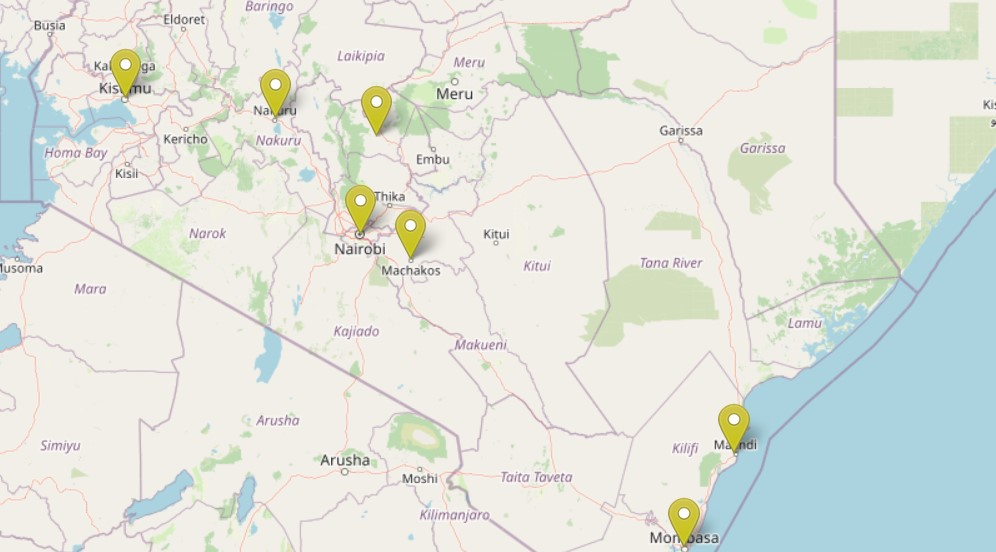
\includegraphics[width=13.83in]{../images/geojson-markers}

All cities were marked yellow, irrespective of their population or jurisdictional significance. But before we raise the alarm on this, what was the purpose of the \texttt{pointToLayer()} function? According to the Leaflet guide, the \texttt{pointToLayer()} function is a special function for GeoJSON variables that species how they should be drawn. In this case and in any other case, it passes the commands in the body, such as \texttt{return\ L.marker...} for every marker point at its Lat-Lon coordinates.

\hypertarget{differentiate-custom-markers-on-a-webmap}{%
\section{Differentiate custom markers on a webmap}\label{differentiate-custom-markers-on-a-webmap}}

Now to our spirited arguments. Not all cities are equal. We would appreciate if the markers would differentiate the cities to a particular variable, say population. By the way, size of cities is determined by population. The below code shall differiante cities by circle markers before we go back to normal markers when we touch the \texttt{fetch()} function again.

Comment out the earlier code and insert this:

\begin{verbatim}
L.geoJSON(cities, {
  pointToLayer: function (feature, latlng) {
    if (feature.properties.Population <= 250000) {
      return L.circleMarker(latlng, {
        radius: 4,
        fillColor: '#FFFF00',
        color: '#000',
        weight: 1,
        opacity: 1,
        fillOpacity: 0.8  
      });
    } else if (feature.properties.Population <= 800000) {
      return L.circleMarker(latlng, {
        radius: 8,
        fillColor: '#ff9900',
        color: '#000',
        weight: 1,
        opacity: 1,
        fillOpacity: 0.8  
      });
    } else {
      return L.circleMarker(latlng, {
        radius: 12,
        fillColor: '#FF0000',
        color: '#000',
        weight: 1,
        opacity: 1,
        fillOpacity: 0.8  
      });
    }
    
  }
}).bindPopup(function (layer) {
  return `City: ${layer.feature.properties.City},<br>
  Population: ${layer.feature.properties.Population}`;
}).addTo(map);
\end{verbatim}

What you get is a map that has different circle markers according to the respective city's population. This time round, the \texttt{pointToLayer()} function body worked with \textbf{if/else if} statement to differentiate the radius and color of each circle marker. Under the \textbf{if/else if} code statement block, different circle marker specifications of radius and fillColor were inserted for each population category. Any city with a population beyond 800000 was fitted into the \texttt{else} block.

\begin{Shaded}
\begin{Highlighting}[]
\NormalTok{knitr}\SpecialCharTok{::}\FunctionTok{include\_graphics}\NormalTok{(}\FunctionTok{rep}\NormalTok{(}\StringTok{"D:/gachuhi/my{-}leaflet/images/geojson{-}diff1.jpg"}\NormalTok{))}
\end{Highlighting}
\end{Shaded}

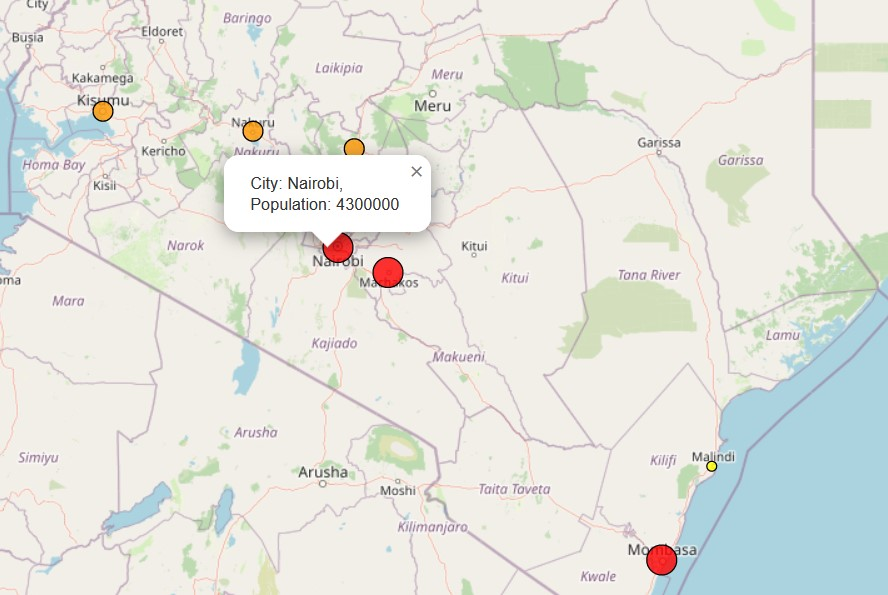
\includegraphics[width=12.33in]{../images/geojson-diff1}

This brings us to why we changed the population values from strings to integers. If we were to work with their former values of strings, any value beyond 1, 000, 000 would receive the settings of \texttt{feature.properties.Population\ \textless{}=\ 250000} that is, color yellow and radius yellow. This is because even though 1 million is by far larger than 250, 000 or 800, 000, because it starts with a 1, it shall be considered even less than 250, 000! This is because when ordering strings in JavaScript, they are by default ordered by the first character. The same case applies to digits 1 to 9. Value 1 will always be inferior to 2, 7, 9 and any other number in between irrespective of whether its a million or a billion.

In the next code sample, we shall create city markers but their populations differentiated with new markers icons we created of yellow, orange and red.

\begin{verbatim}
L.geoJSON(cities, {
  pointToLayer: function (feature, latlng) {
    if (feature.properties.Population <= 250000) {
      return L.marker(latlng, {
        icon: yellowIcon 
      });
    } else if (feature.properties.Population <= 800000) {
      return L.marker(latlng, {
        icon: orangeIcon 
      });
    } else {
      return L.marker(latlng, {
        icon: redIcon 
      });
    }
    
  }
}).bindPopup(function (layer) {
  return `City: ${layer.feature.properties.City},<br>
  Population: ${layer.feature.properties.Population}`;
}).addTo(map);
\end{verbatim}

\begin{Shaded}
\begin{Highlighting}[]
\NormalTok{knitr}\SpecialCharTok{::}\FunctionTok{include\_graphics}\NormalTok{(}\FunctionTok{rep}\NormalTok{(}\StringTok{"D:/gachuhi/my{-}leaflet/images/geojson{-}diff2.jpg"}\NormalTok{))}
\end{Highlighting}
\end{Shaded}

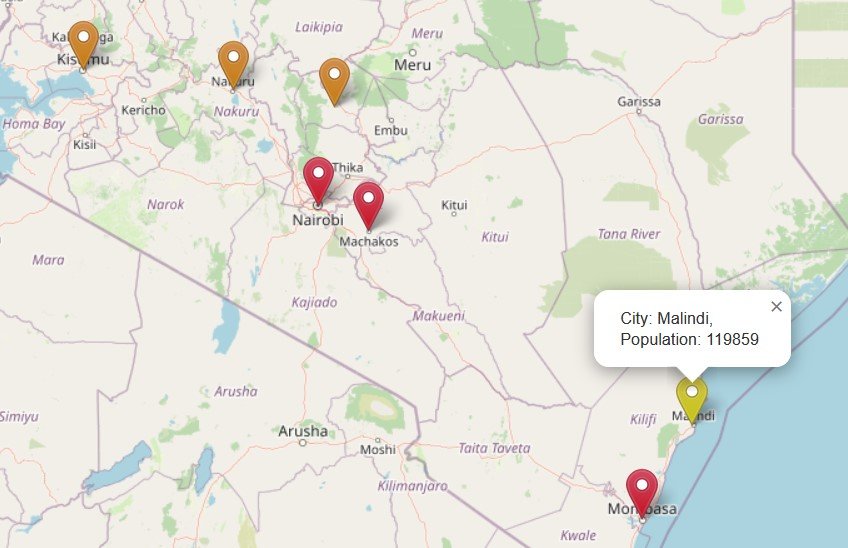
\includegraphics[width=11.78in]{../images/geojson-diff2}

In the above map, our preceding code has differentiated large cities with populations above 800, 000 with a red marker, those with populations below 250, 000 with a yellow marker and those between with an orange marker. In all cases, our \texttt{bindPopup()} still contains the same settings to show both the city name and population.

The \texttt{pointToLayer()} function was passed function that return a specific \texttt{L.marker} with Lat-Lon coordinates for each respective marker retrieved of course, only that the \texttt{icon} key was assigned a different marker icon variable corresponding to each city's population as the value. That's the trick that assigns a different marker to each city as per its population.

\hypertarget{using-fetch}{%
\section{Using fetch}\label{using-fetch}}

Remember how \texttt{fetch} helped us retrieve data from a server in a previous chapter. Whereas we won't repeat the entire process again (you can breathe a sigh of relief), the same iterations of differentiating a marker icon can also be inserted in \texttt{fetch}, right within the options of \texttt{L.geoJson(data,\ \{options\})}.

\begin{verbatim}
fetch("https://raw.githubusercontent.com/sammigachuhi/geojson_files/main/cities-geojson2.geojson.txt")
    .then((response) =>{
        return response.json()
    })
    .then((data) => {
        L.geoJson(data, {
          pointToLayer: function (feature, latlng) {
            if (feature.properties.Population <= 250000) {
              return L.marker(latlng, {
                icon: yellowIcon 
              });
            } else if (feature.properties.Population <= 800000) {
              return L.marker(latlng, {
                icon: orangeIcon 
              });
            } else {
              return L.marker(latlng, {
                icon: redIcon 
              });
            }
            
          }
        }).bindPopup((layer) => {
            return `City: ${layer.feature.properties.City},<br>
            Population: ${layer.feature.properties.Population}`}).addTo(map);
    })
    .catch((error) => {
        console.log(`This is the error: ${error}`)
    })
\end{verbatim}

It works but don't take my word for it. Just paste and see.

\hypertarget{unique-custom-markers}{%
\section{Unique custom markers}\label{unique-custom-markers}}

This part may not be necessary, but it is just to show you that there are various markers apart from the defaults provided by Leaflet. One can create custom markers outside of leaflet using the {[}Leaflet.Awesome.Markers plugin{]}. Just like in the case of Ajax, you will need to install the path to the dependencies in the html document \texttt{map.html} using \texttt{\textless{}script\textgreater{}}. Insert the following \texttt{\textless{}script\textgreater{}} tags into \texttt{map.html}.

\begin{verbatim}
<script src="Leaflet.awesome-markers-2.0-develop\Leaflet.awesome-markers-2.0-develop\dist\leaflet.awesome-markers.js"></script>

<script src="Leaflet.awesome-markers-2.0-develop\Leaflet.awesome-markers-2.0-develop\dist\leaflet.awesome-markers.css"></script>
\end{verbatim}

And also this \texttt{\textless{}link\textgreater{}} tag:

\begin{verbatim}
<link href="http://netdna.bootstrapcdn.com/font-awesome/4.0.0/css/font-awesome.css" rel="stylesheet"> 
\end{verbatim}

To make the best use of time, following the example on their site, we simply replace our \texttt{icon} values with the new \texttt{L.AwesomeMarkers.icon} for each population category, and also tweaked the colors for each to match those of our previous markers. We assumed that big cities have the best malls, the medium cities, those with above a population of 250, 000 but a peak of 800, 000 to also have good coffee places, and those with populations of less than a quarter million have respectable industries. We assume fair play has been exercised in our assumptions. Here is the code.

\begin{verbatim}
L.geoJSON(cities, {
    pointToLayer: function (feature, latlng) {
      if (feature.properties.Population <= 250000) {
        return L.marker(latlng, {
          icon: L.AwesomeMarkers.icon({icon: 'cog', prefix: 'fa', markerColor: 'purple', iconColor: 'yellow'}) 
        });
      } else if (feature.properties.Population <= 800000) {
        return L.marker(latlng, {
          icon: L.AwesomeMarkers.icon({icon: 'coffee', prefix: 'fa', markerColor: 'red', iconColor: 'orange'}) 
        });
      } else {
        return L.marker(latlng, {
          icon: L.AwesomeMarkers.icon({icon: 'shopping-cart', prefix: 'fa', markerColor: 'blue', iconColor: 'red'})
        });
      }
      
    }
  }).bindPopup(function (layer) {
    return `City: ${layer.feature.properties.City},<br>
    Population: ${layer.feature.properties.Population}`;
  }).addTo(map);
\end{verbatim}

\begin{Shaded}
\begin{Highlighting}[]
\NormalTok{knitr}\SpecialCharTok{::}\FunctionTok{include\_graphics}\NormalTok{(}\FunctionTok{rep}\NormalTok{(}\StringTok{"D:/gachuhi/my{-}leaflet/images/extra{-}markers.jpg"}\NormalTok{))}
\end{Highlighting}
\end{Shaded}

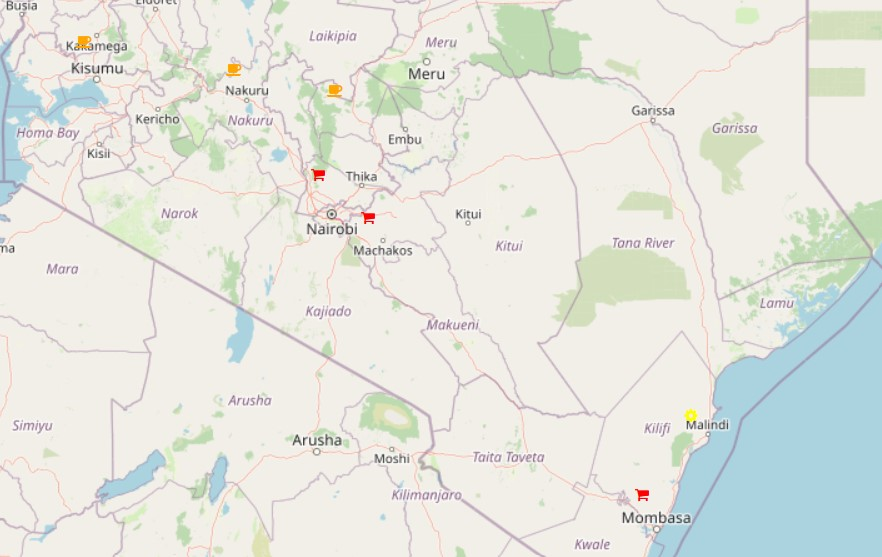
\includegraphics[width=12.25in]{../images/extra-markers}

The custom markers are also clickable!

\hypertarget{image-overlays}{%
\section{Image overlays}\label{image-overlays}}

Sometimes an image can act as good a marker as any other displayed so far. Overlaying images on a map is fairly easy, and if in a rush, here is the code:

\begin{verbatim}
// Image overlays
var imageUrl = 'https://pbs.twimg.com/media/DddQBk5WsAAlbdJ?format=jpg&name=large';
var errorOverlayUrl = 'https://pbs.twimg.com/media/DddQBk5WsAAlbdJ?format=jpg&name=large';
var altText = 'The Galton - Fenzi Memorial: Source: Google and Twitter';
var latLngBounds = L.latLngBounds([[-1.2861259,36.8172709], [-1.2886193,36.8230413]]);

var imageOverlay = L.imageOverlay(imageUrl, latLngBounds, {
    opacity: 0.8,
    errorOverlayUrl: errorOverlayUrl,
    alt: altText,
    interactive: true
}).addTo(map);

\end{verbatim}

However, find an image of one location over the wide earth can be tricky and tiring, so we envelope it with a rectangle plus use \texttt{map.fitBounds} to zoom to where our image is placed.

\begin{verbatim}
L.rectangle(latLngBounds).addTo(map);
map.fitBounds(latLngBounds);
\end{verbatim}

\begin{Shaded}
\begin{Highlighting}[]
\NormalTok{knitr}\SpecialCharTok{::}\FunctionTok{include\_graphics}\NormalTok{(}\FunctionTok{rep}\NormalTok{(}\StringTok{"D:/gachuhi/my{-}leaflet/images/geltan{-}fenzi.jpg"}\NormalTok{))}
\end{Highlighting}
\end{Shaded}

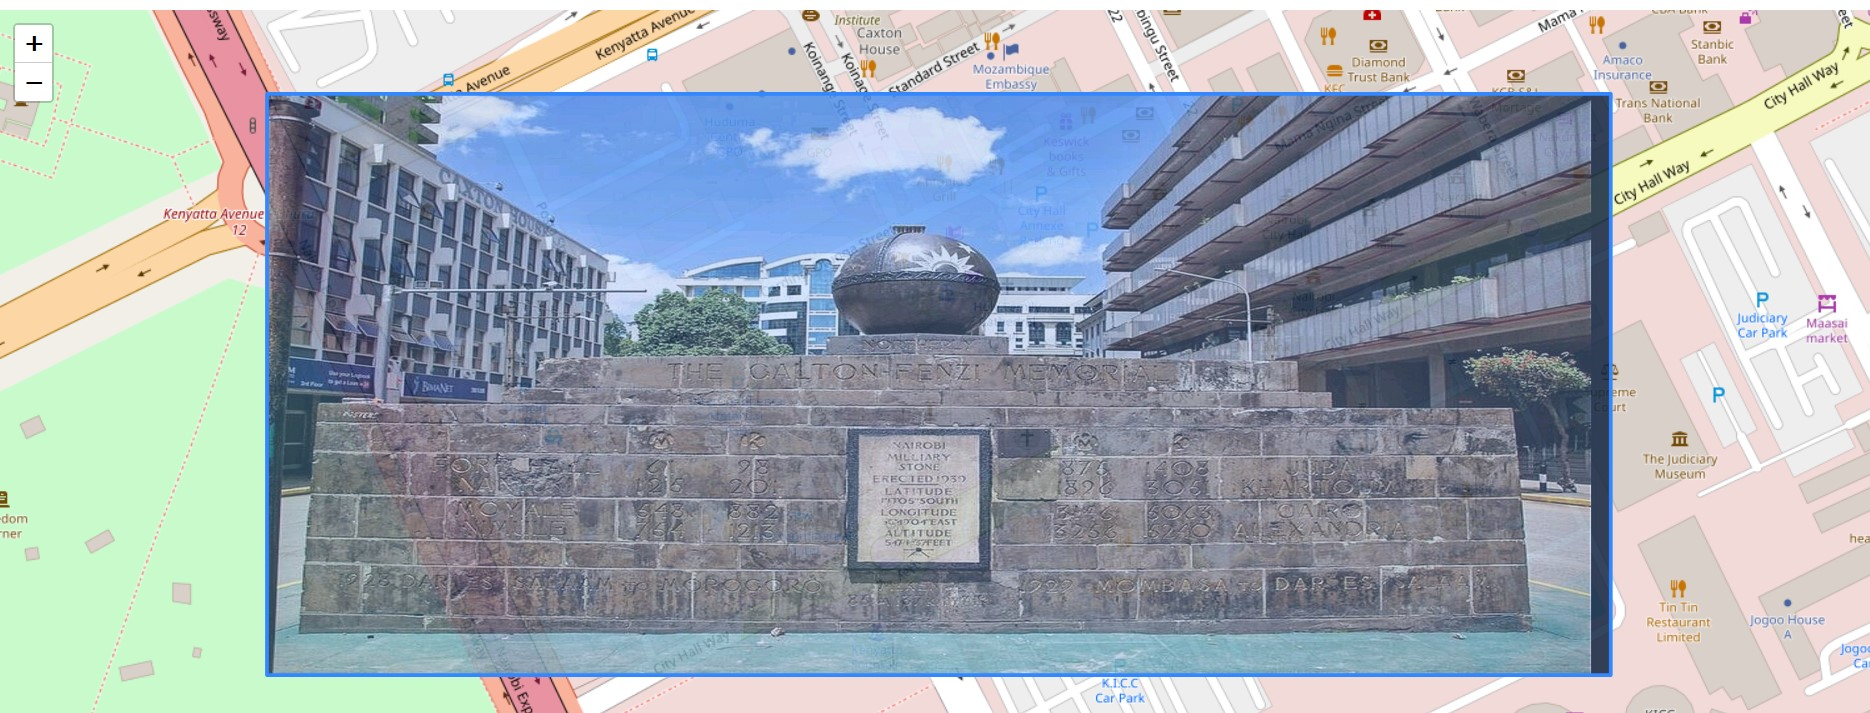
\includegraphics[width=25.97in]{../images/geltan-fenzi}

Mind you that landmark was set up in 1939 in honour of Lionel Douglas Galton-Fenzi who was the first motorist to drive from Nairobi to Mombasa when all that existed was dirt track laden with wild animals. Yours truly has also heard it contains bearings to various East African cities. Despite being at a point where I normally alight, I've never paid much attention to it nor its bearings. Next time, I will be keen.

Anyway, here is a quick breakdown of the attributes used in \texttt{L.imageOverlay}. We understand we have taken a lot of your time on so much a simple chapter, so we will be swift. The \texttt{var\ latLngBounds} uses the \texttt{L.latLngBounds} class to set the lat-lon coordinates. Notice they are two coordinate lists bound with a single \texttt{{[}{]}}. Your brain will get used to this in time. If you don't enclose the two coordinates with \texttt{{[}{]}} an error may result. \texttt{var\ ImageUrl} is self explanatory --its the image source and for the rest, here they are:

\begin{enumerate}
\def\labelenumi{\arabic{enumi}.}
\item
  \texttt{opacity} - defines the opacity of the image overlay, it equals to 1.0 by default. Decrease this value to make an image overlay transparent and to expose the underlying map layer.
\item
  \texttt{errorOverlayUrl} - is a URL to the overlay image to show in place of the overlay that failed to load.
\item
  \texttt{alt} - sets the HTML alt attribute to provide an alternative text description of the image. Alternative text is essential information for screen reader users. It can also benefit people during poor network connectivity, in the case the image fails to load. Moreover, it can improve the SEO of a website.
\item
  \texttt{interactive} - is false by default. If true, the image overlay will emit mouse events when clicked or hovered.
\end{enumerate}

\hypertarget{creating-an-interactive-choropleth-map}{%
\chapter{Creating an interactive choropleth map}\label{creating-an-interactive-choropleth-map}}

\hypertarget{what-is-a-choropleth-map}{%
\section{What is a choropleth map?}\label{what-is-a-choropleth-map}}

We will now move from markers to something larger than life --choropleth maps. What the heck are choropleth maps. Geographers will roll their over this term because they have come across almost throughout their career, but for the sake new readers, a \href{https://datavizcatalogue.com/methods/choropleth.html}{choropleth map} is a map whose geographical areas or regions are colored, shaded or patterned in relation to a data variable. If you have seen map that has disaggregated election results to states or provinces, and draped the winning candidate or party by color on the particular state, then that's a choropleth map. They mostly appear in election broadcasts, especially those of a national kind. In this chapter, we will create a choropleth map of Kenyan counties, and make it interactive by leveraging the area and population characteristics of each county.

\hypertarget{creating-a-choropleth-map-the-start}{%
\section{Creating a choropleth map: the start}\label{creating-a-choropleth-map-the-start}}

Obviously by now, without going into much details, you can now create a basic leaflet map blindfolded. Anyway, seeing is believing, so lets start what we have done several times over. Create another new JavaScript file (I know its repetitive, but enjoy it nevertheless) called \texttt{interactive-choropleth.js}.

In order to cheer you up with the monotonous opening statement in our many JavaScript files, we shall use a new tile layer.

\begin{verbatim}
var map = L.map('myMap').setView([0.3556, 37.5833], 6.5);

L.tileLayer('https://{s}.tile-cyclosm.openstreetmap.fr/cyclosm/{z}/{x}/{y}.png', {
    maxZoom: 20,
    attribution: '<a href="https://github.com/cyclosm/cyclosm-cartocss-style/releases" title="CyclOSM - Open Bicycle render">CyclOSM</a> | Map data: &copy; <a href="https://www.openstreetmap.org/copyright">OpenStreetMap</a> contributors'
}).addTo(map); // the CyclOSM tile layer available from Leaflet servers
\end{verbatim}

Remember us mentioning that Leaflet has other \href{https://leaflet-extras.github.io/leaflet-providers/preview/}{tile layer servers}? Here we have just used another, specifically CyclOSM tile layers.

Now to the big part. The geojson files. We would like to mention it was quite a hustle to set up the geojson file in a manner accessible with JavaScript's Fetch API. Only when we converted the geojson to json, we were able to successfully view it using \texttt{fetch}. The raw json file for our Kenyan counties which we shall use in creating a choropleth map are available from \href{https://raw.githubusercontent.com/sammigachuhi/geojson_files/main/counties_json.json}{here}.

Let's fetch the counties json file and keep quiet.

\begin{verbatim}
fetch("https://raw.githubusercontent.com/sammigachuhi/geojson_files/main/counties_json.json")
    .then((response) =>{
        return response.json()
    })
    .then((data) => {
        L.geoJson(data, {style: style}).addTo(map);
    })
    .catch((error) => {
        console.log(`This is the error: ${error}`)
    })
    
\end{verbatim}

So far, you should get a result like below.

\begin{Shaded}
\begin{Highlighting}[]
\NormalTok{knitr}\SpecialCharTok{::}\FunctionTok{include\_graphics}\NormalTok{(}\FunctionTok{rep}\NormalTok{(}\StringTok{"D:/gachuhi/my{-}leaflet/images/kenya\_json.jpg"}\NormalTok{))}
\end{Highlighting}
\end{Shaded}

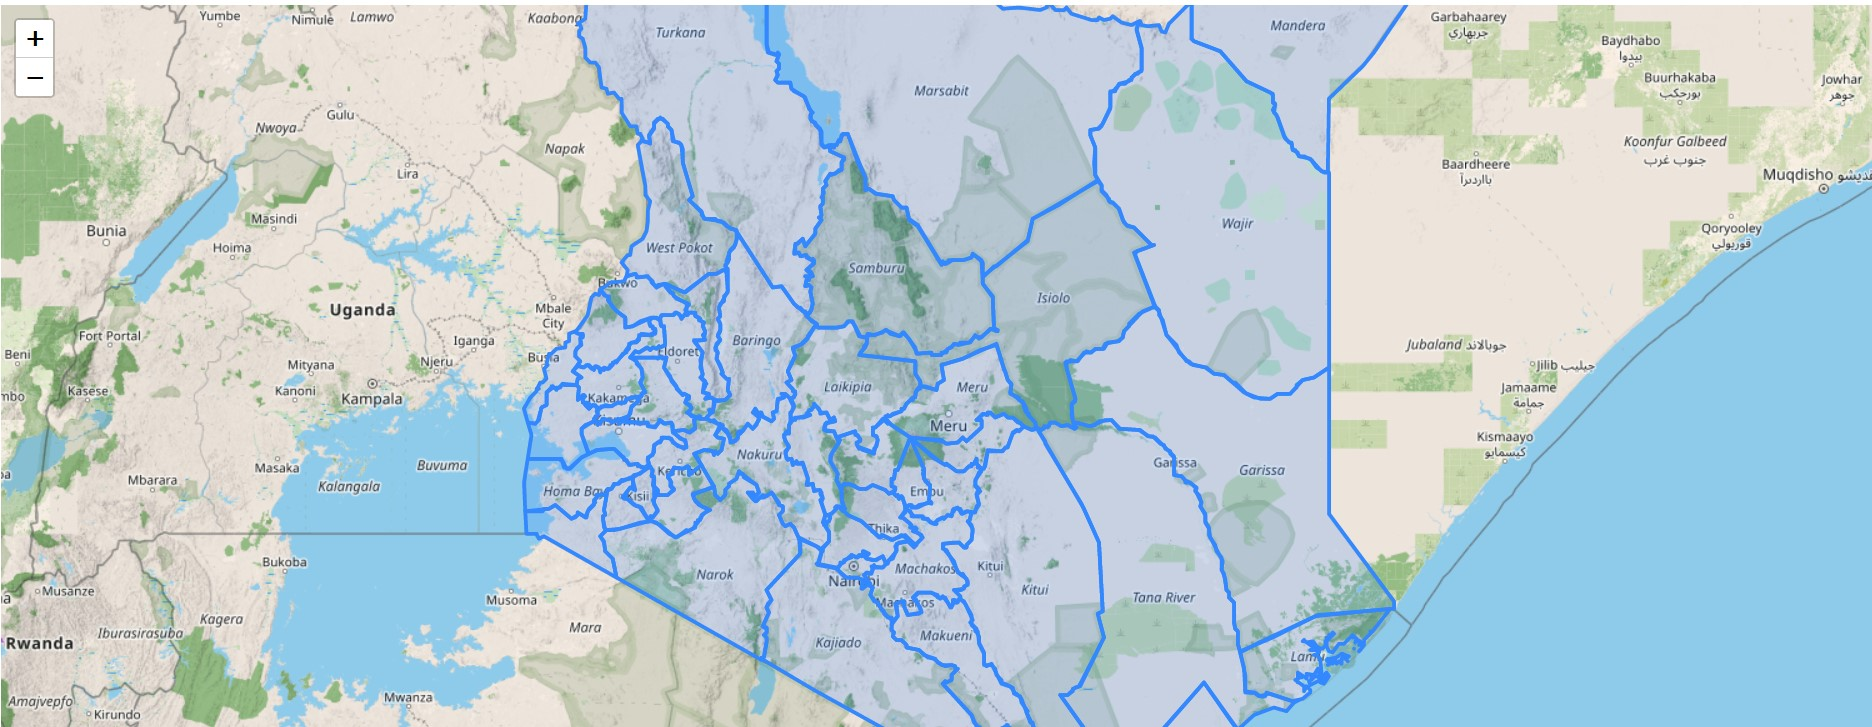
\includegraphics[width=26in]{../images/kenya_json}

\hypertarget{coloring-the-counties}{%
\section{Coloring the counties}\label{coloring-the-counties}}

Alright, we have been able to load our json file to a Leaflet map. However, it looks dull and provides no meaningful information to the casual observation. When making maps, aim to provide information at lightning speed. That is, inform the reader at fast glance. The code snippets that follow have been heavily borrowed from Volodymyr's interactive choropleth tutorial.

First, let create a function that sets a color hex code for each population category. We used color brewer for this, as did Volodymyr in his tutorial.

Take a look at this code and we shall explain.

\begin{verbatim}
//// Adding some color
function getColor(d) {
    return d > 1400 ? '#8c2d04' :
            d > 700 ? '#cc4c02' :
            d > 400 ? '#ec7014' :
            d > 100 ? '#fe9929' :
            d >  50 ?  '#fec44f':
            d > 25 ?   '#fee391':
                       '#ffffd4';
}
\end{verbatim}

The above function uses a question mark \texttt{?} to act as the if\ldots else statement. In JavaScript terms, it is known as a \href{https://www.freecodecamp.org/news/how-the-question-mark-works-in-javascript/}{ternary operator}. What's that? How does it work? We can answer the second more arguably. For the former, we can only go as far as the definition.

How the ternary operator works is that any statement to the right of the \texttt{?} is returned as true if it agrees with the value to the left of the \texttt{?}. Reread that statement again. If the value to the right of the \texttt{?} is false, then the value to the right of the colon \texttt{:} is returned. Reread that last statement again.

If it still sounds fuzzy, the below image should help (adapted from \href{https://www.freecodecamp.org/news/how-the-question-mark-works-in-javascript/}{FreeCodeCamp}).

\begin{Shaded}
\begin{Highlighting}[]
\NormalTok{knitr}\SpecialCharTok{::}\FunctionTok{include\_graphics}\NormalTok{(}\FunctionTok{rep}\NormalTok{(}\StringTok{"D:/gachuhi/my{-}leaflet/images/ternary.png"}\NormalTok{))}
\end{Highlighting}
\end{Shaded}

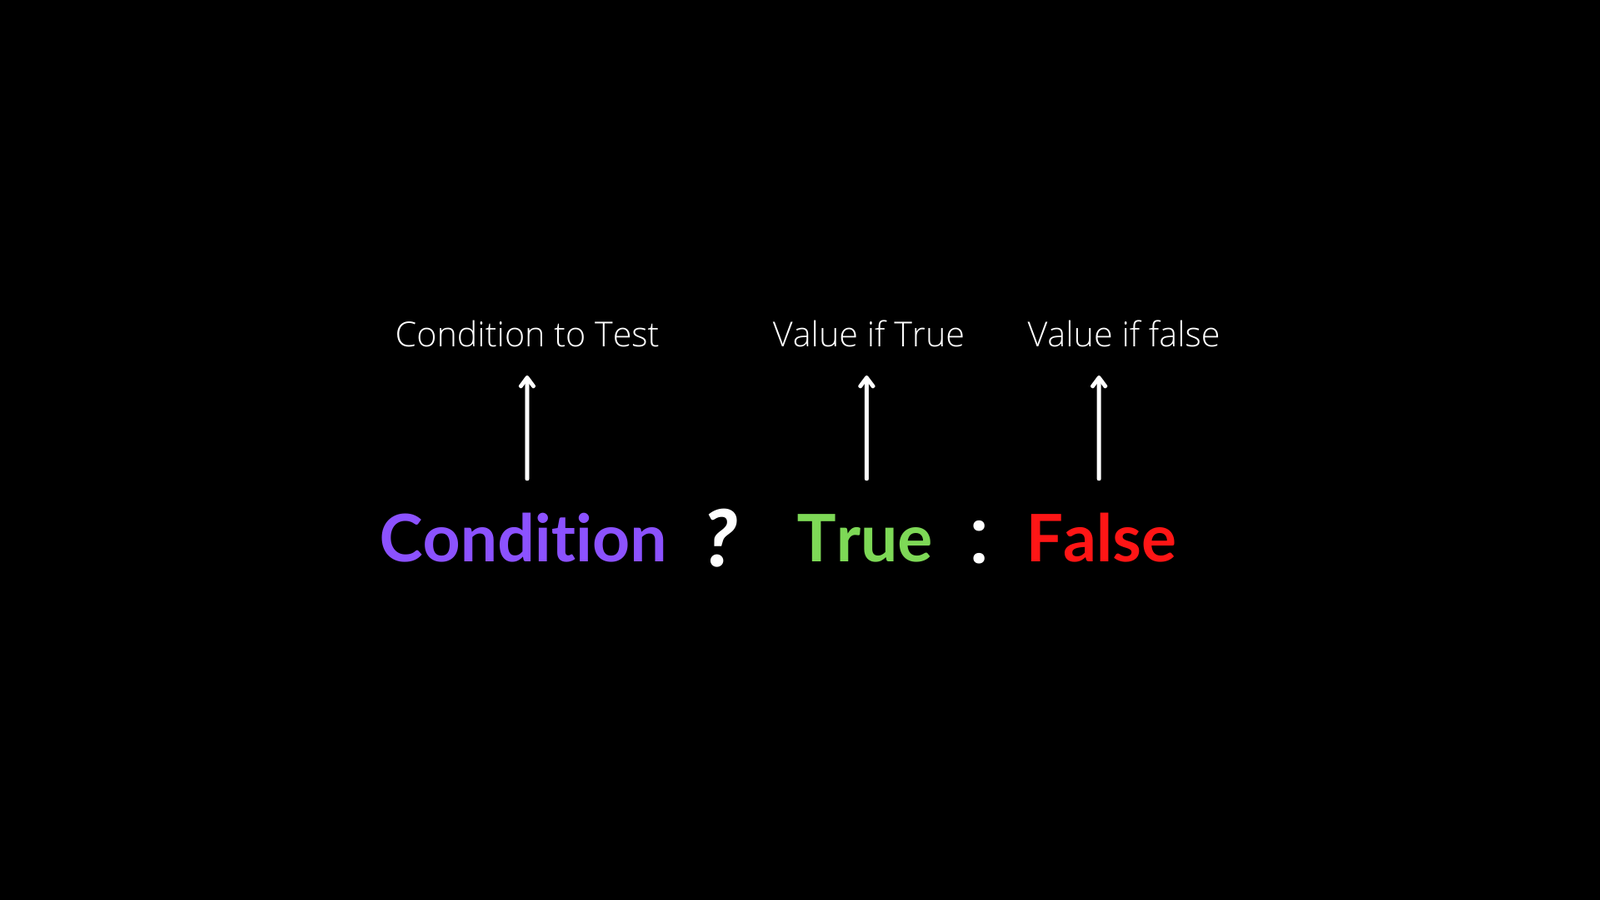
\includegraphics[width=22.22in]{../images/ternary}

Now that we've created the function of setting colors to our json file on leaflet, we next also have to \emph{create} a function that does to the GeoJSON file itself. Luckily, we have the \textbf{style} \href{https://leafletjs.com/reference.html\#geojson-style}{option from Leaflet} which is styles GeoJSON lines and polygons using features from the GeoJSON file itself. We saw it in \protect\hyperlink{using-geojson-in-leaflet}{Chapter} and we shall also use it here.

\begin{verbatim}
var style = ((feature)=> {
    return {
        fillColor: getColor(feature.properties.Pop_Density),
        weight: 2,
        opacity: 1,
        color: 'gray',
        fillOpacity: 0.5
    }
})
\end{verbatim}

The above is an arrow function. Unlike regular JavaScript function declarations (function ()), we remove the \texttt{function} keyword, enclose everythin in brackets and put an arrow \texttt{=\textgreater{}} between the parameter brackets and function body. That's just it. Arrow functions aren't so hard!

Remember we assign the arrow function to a variable called \texttt{style} since we will parse it to the \texttt{L.geoJson} class. Just to keep things neat.

Finally, we add the \texttt{style} variable to the \textbf{style} option of \texttt{L.geoJson} class.

\begin{verbatim}
fetch("https://raw.githubusercontent.com/sammigachuhi/geojson_files/main/counties_json.json")
    .then((response) =>{
        return response.json()
    })
    .then((data) => {
        L.geoJson(data, {style: style}).addTo(map);
    })
    .catch((error) => {
        console.log(`This is the error: ${error}`)
    })
    
\end{verbatim}

Since the \textbf{style} option is a key (and also a function), the value will be the \texttt{var\ style} which we created. This value is in and by itself a function that iterates over every county because of the \texttt{getColor(feature.properties.Pop\_Density)} contained in it as the \texttt{fillColor} value!

Enough JavaScript for one day!

\begin{Shaded}
\begin{Highlighting}[]
\NormalTok{knitr}\SpecialCharTok{::}\FunctionTok{include\_graphics}\NormalTok{(}\FunctionTok{rep}\NormalTok{(}\StringTok{"D:/gachuhi/my{-}leaflet/images/choropleth{-}map.jpg"}\NormalTok{))}
\end{Highlighting}
\end{Shaded}

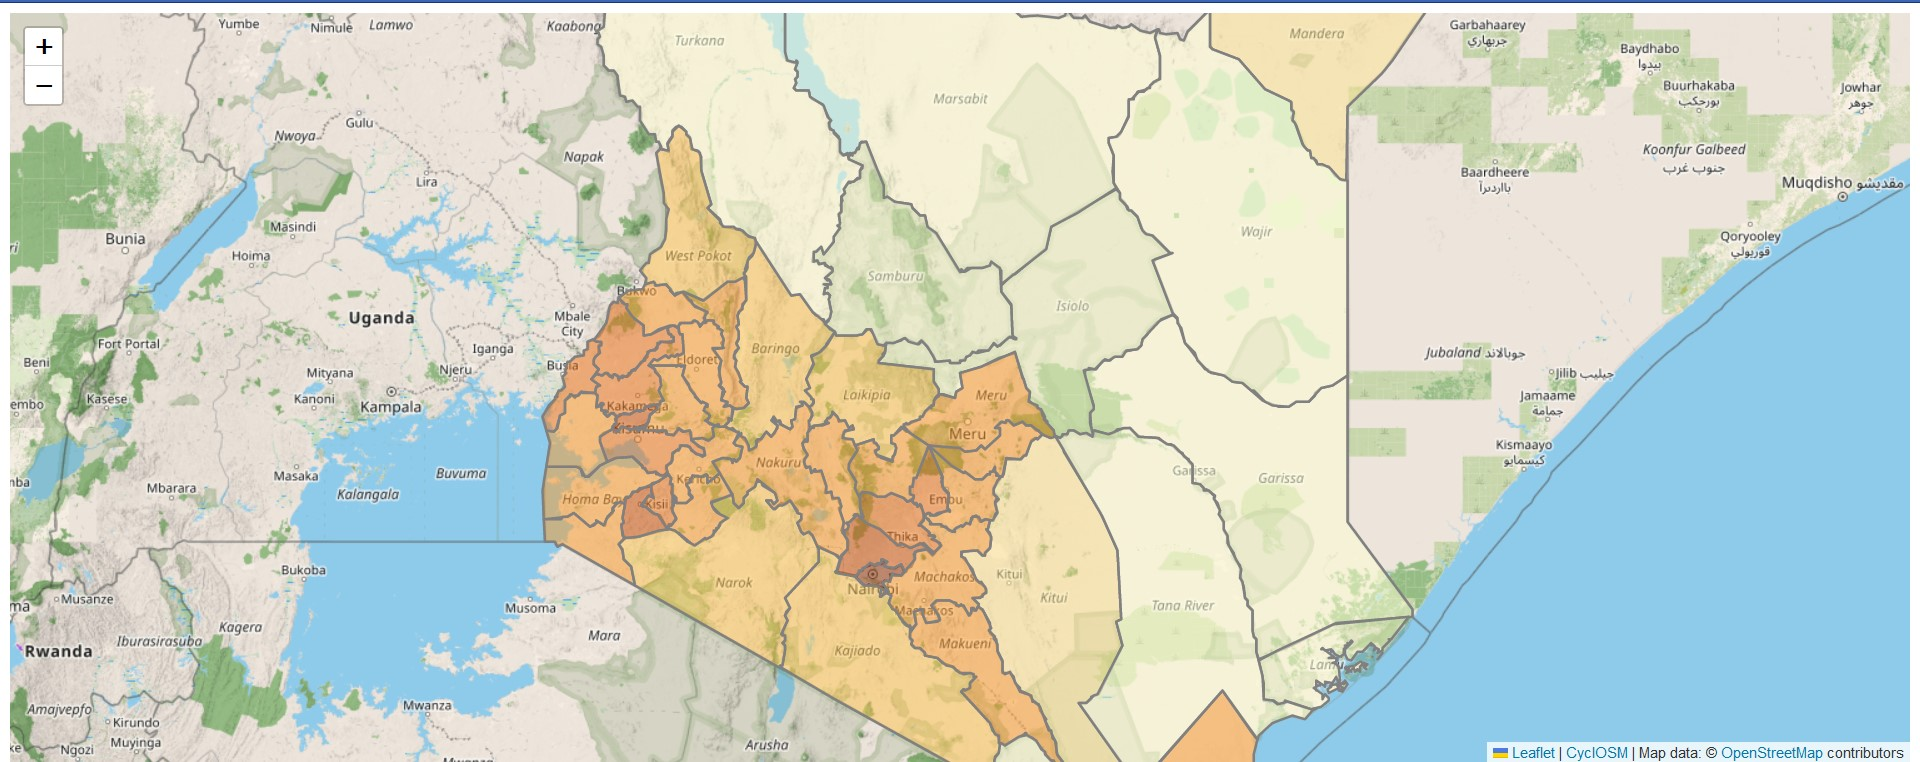
\includegraphics[width=26.67in]{../images/choropleth-map}

Our choropleth map is beginning to take shape.

\hypertarget{highlight-features}{%
\section{Highlight features}\label{highlight-features}}

Going on from where we last left, we would like the choropleth map to highlight counties upon mouse hover, and also display their attributes upon click and zoom to the county! Quite a lot to work for. The counties should also be reset to their default characteristics upon mouse out.

Alright. It seems like we have our hands full.

Let's start simple.

Remember the \texttt{fetch} API we had used in retrieving our json file. We will tweak it a bit by adding the \texttt{var\ geojson} just before calling the \texttt{L.geoJson} class. We shall assing the variable \texttt{geojson} to the \texttt{L.geoJson} class. We know you are raising eyebrows. We shall explain why.

\begin{verbatim}
fetch("https://raw.githubusercontent.com/sammigachuhi/geojson_files/main/counties_json.json")
    .then((response) =>{
        return response.json()
    })
    .then((data) => {
        var geojson;
        geojson = L.geoJson(data, {
            style: style,
            --snip--
    })
\end{verbatim}

We want upon hovering our mouse over each county, that the county is highlighted in white and appear to slightly `pop' out above the rest. To do so, we insert the following code:

\begin{verbatim}

        geojson = L.geoJson(data, {
            style: style,
            onEachFeature: ((feature, layer) => {
                layer.on('mouseover', ((e) => {
                    var layer = e.target;
                
                    layer.setStyle({
                        weight: 5,
                        color: '#FFFFFF',
                        dashArray: '',
                        fillOpacity: 0.7
                    });
                
                    layer.bringToFront();
                }))
                
                
\end{verbatim}

The purpose of \texttt{on} method is to add an event listener. Event listeners in JavaScript are functions that run a code when the browser user interacts with the browser in a specific way. Now what \texttt{on} method does is that \emph{Upon} each layer, we had an event listener known as \texttt{mouseover}. In our case, upon hovering a mouse pointer over our county we want the county hovered over to `pop' out slightly and with a white border.

Since the change in state of an element in HTML is known as an event (denoted as \texttt{e} in our case), the \texttt{e.target} property returns the element on which the event is occurring on. Since it's a particular county in our case, we proceed to change its symbology through the parameters in \texttt{setStyle} function. Thereafter we use the \texttt{bringToFront} method to make the element in which the event has happened on to `pop' out above the rest.

Remember we had mentioned we also want the counties to be reset to their default status when one hovers out to some other county or outside the map altogether. The following code does the job.

\begin{verbatim}
layer.on('mouseout', function() {
                    geojson.resetStyle(this);
                })
\end{verbatim}

We use the \texttt{resetStyle} function to return the layer to their default but there is a twist. However, in this case, we add the argument \texttt{this} in parenthesis to refer to the element that was received. In other words, when the mouse `hovers out' of a county, the element will revert to its original symbology. That particular element is parsed to \texttt{resetStyle} through \texttt{this} argument in parenthesis.

Before, we end this monologue, we ensure we pass the variable \texttt{geojson} to \texttt{resetStyle} function or else it won't work. This is how it is explained in the leaflet documentation as well as the \emph{modus operandi} \href{https://stackoverflow.com/questions/35072630/why-doesnt-resetstyle-of-leaflet-work-for-me}{here} and \href{https://stackoverflow.com/questions/21029533/reset-style-on-leaflet-polygon-on-click}{here}.

Finally, we mentioned we want to zoom to a particular county upon clicking it. The following code fits our map to the bounds of a particular county that was clicked. Note that \texttt{fitBounds} is parsed \texttt{getBounds} which gets the boundaries of the county clicked upon, as referenced by \texttt{e.target}.

\begin{verbatim}
layer.on('click', ((e) => {
                    map.fitBounds(e.target.getBounds())
                }))
\end{verbatim}

\begin{Shaded}
\begin{Highlighting}[]
\NormalTok{knitr}\SpecialCharTok{::}\FunctionTok{include\_graphics}\NormalTok{(}\FunctionTok{rep}\NormalTok{(}\StringTok{\textquotesingle{}D:/gachuhi/my{-}leaflet/images/highlightable{-}map.jpg\textquotesingle{}}\NormalTok{))}
\end{Highlighting}
\end{Shaded}

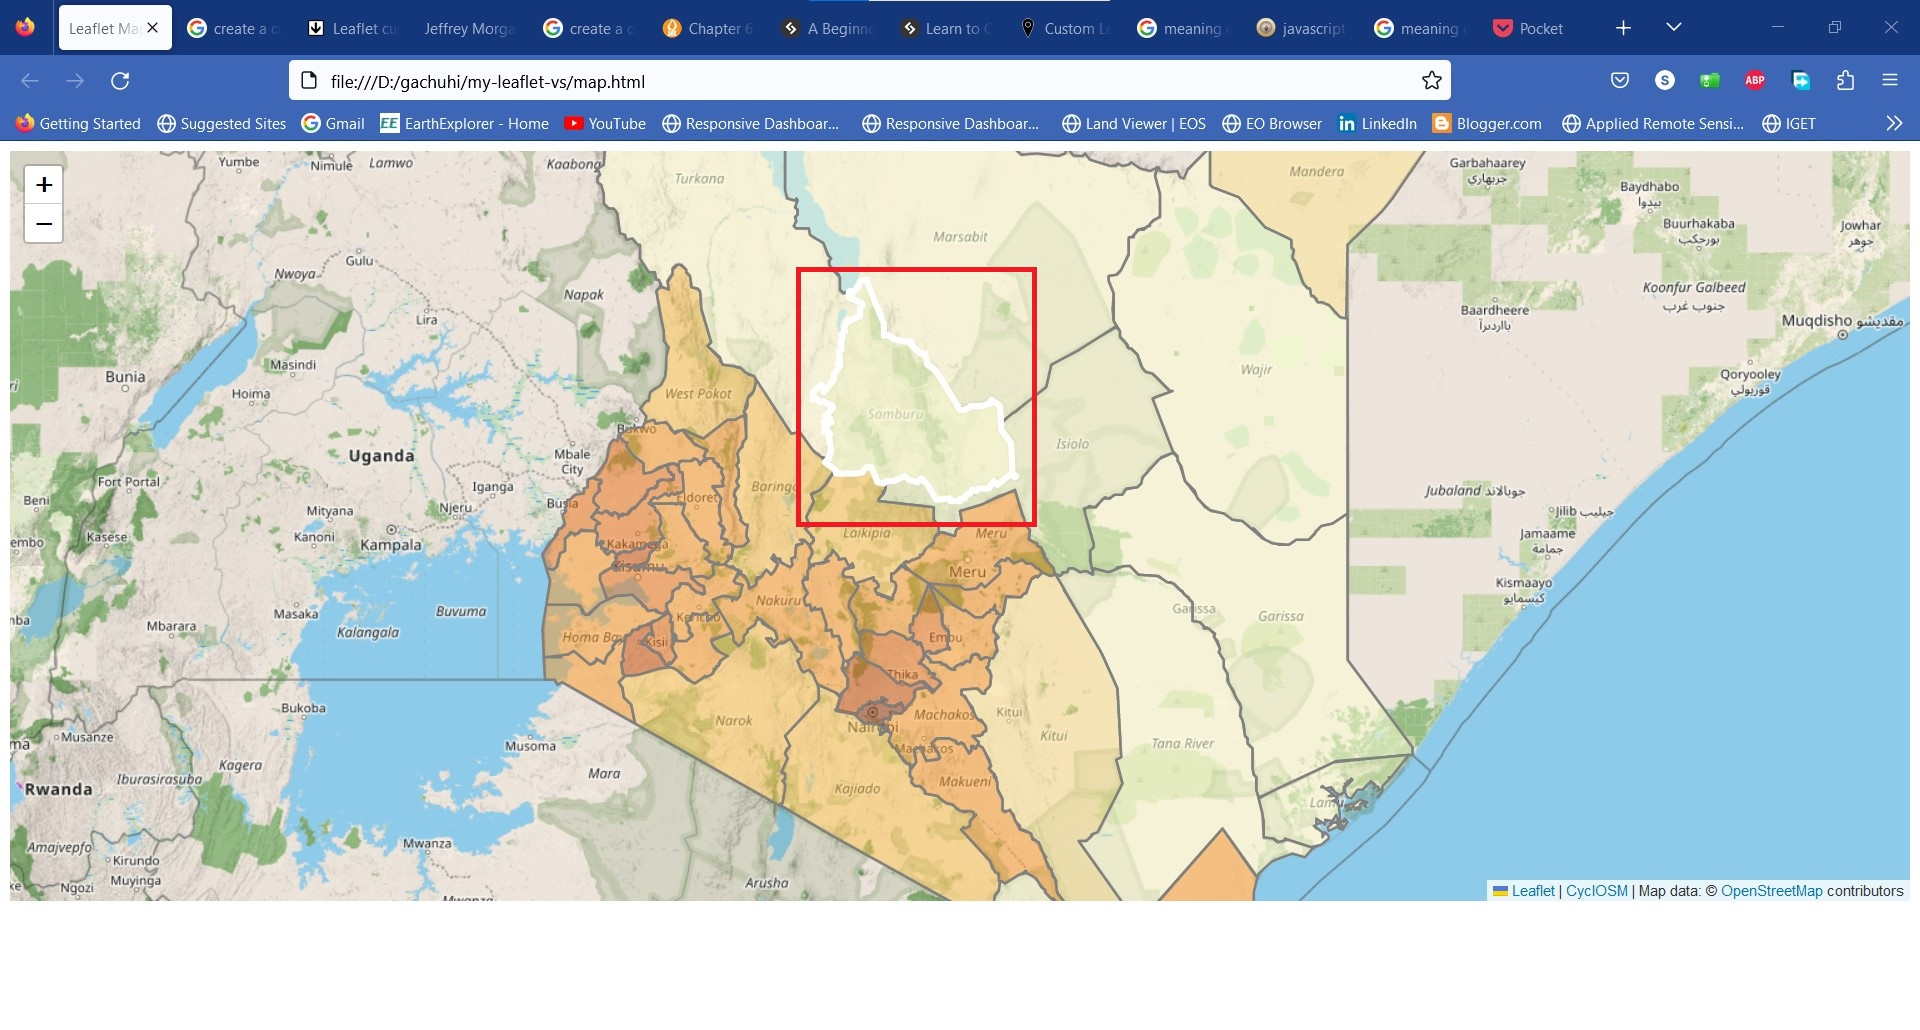
\includegraphics[width=26.67in]{../images/highlightable-map}

Your code within the \texttt{fetch} API should look like this.

\begin{verbatim}
fetch("https://raw.githubusercontent.com/sammigachuhi/geojson_files/main/counties_json.json")
    .then((response) =>{
        return response.json()
    })
    .then((data) => {
        var geojson;
        geojson = L.geoJson(data, {
            style: style,
            onEachFeature: ((feature, layer) => {
                layer.on('mouseover', ((e) => {  // highlight county on mouse hover
                    var layer = e.target;
                
                    layer.setStyle({
                        weight: 5,
                        color: '#FFFFFF',
                        dashArray: '',
                        fillOpacity: 0.7
                    });
                
                    layer.bringToFront();
                }))

                layer.on('mouseout', function () { // return to original symbology upon mouse hover out
                    geojson.resetStyle(this);
                })

                layer.on('click', ((e) => {  // Zoom to county upon clicking it
                    map.fitBounds(e.target.getBounds())
                }))

            })
        }).addTo(map);
    })
    .catch((error) => {
        console.log(`This is the error: ${error}`)
    })
\end{verbatim}

Such a monolithic code.

\hypertarget{creating-a-custom-info}{%
\section{Creating a custom info}\label{creating-a-custom-info}}

I hope you took a break. If not, take a one good look at the above image for some soothing effects for the sorrow begotten so far.

The following code adds a custom info control to the map. Think of a control as an UI element that allows interactivity with the map. Our custom control info shall provide details of the name, total population and population density.

\begin{verbatim}
// Add control
var info = L.control();

info.onAdd = function (map) {
    this.div = L.DomUtil.create('div', 'info');
    this.update();
    return this.div;
};

// Method that we will use to update the control based on feature properties passed
info.update = function (props) {
    this.div.innerHTML = '<h4>Kenya Population Density</h4>' + (props ? 
        '<b>' + props.ADM1_EN + '</br><br />' + 'Total Population' + '<br>' + props.County_pop + '<br> <br>' + 
        props.Pop_Density + ' people / km<sup>2</sup>': 'Hover over state')
};

info.addTo(map);
\end{verbatim}

That's both scary and cool at the same time. I want you to have the last. When thrown an incomprehensible code, acknowledge the complexity, and think of it as a cool graphic (or graffiti)!

Okay. Let's go through the above code bit by bit as best as we (hopefully!) can.

\texttt{var\ info\ =\ L.control();}

The above creates a variable \texttt{info} that holds the base class \texttt{L.control()} for all map controls. For example, \texttt{L.control.zoom} creates a zoom control in the map.

\begin{verbatim}
info.onAdd = function (map) {
    this.div = L.DomUtil.create('div', 'info');
    this.update();
    return this.div;
};
\end{verbatim}

Returns the DOM element for the control and creates a \texttt{\textless{}div\textgreater{}} with class \texttt{info}. This is done through the help of \texttt{L.DomUtil} which, according to the Leaflet website, provides utility functions to work with the DOM\footnote{The Document Object Model (DOM) is the data representation of the objects that comprise the structure and content of a document on the web.}. Actually, this new \texttt{\textless{}div\textgreater{}} of class \texttt{info} is created when you fire up your browser but obviously not in your actual \texttt{map.html} file.

\begin{Shaded}
\begin{Highlighting}[]
\NormalTok{knitr}\SpecialCharTok{::}\FunctionTok{include\_graphics}\NormalTok{(}\FunctionTok{rep}\NormalTok{(}\StringTok{\textquotesingle{}D:/gachuhi/my{-}leaflet/images/div{-}info{-}element.jpg\textquotesingle{}}\NormalTok{))}
\end{Highlighting}
\end{Shaded}

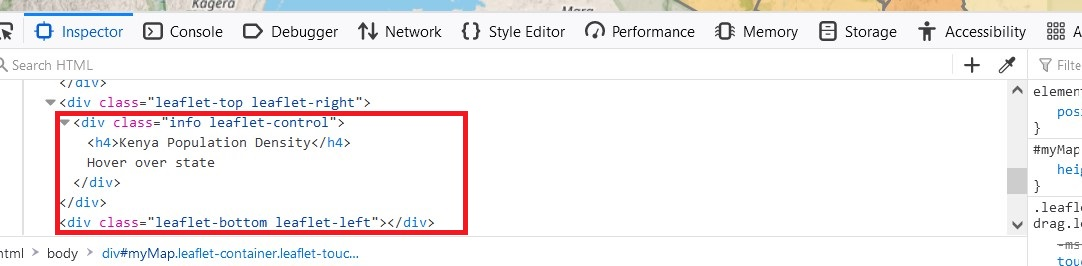
\includegraphics[width=15.03in]{../images/div-info-element}

Trust me it wasn't there before. What \texttt{this.update()} does is return the update function that follows with the properties for each county, and then returns it.

\begin{verbatim}
// Method that we will use to update the control based on feature properties passed
info.update = function (props) {
    this.div.innerHTML = '<h4>Kenya Population Density</h4>' + (props ? 
        '<b>' + props.ADM1_EN + '</br><br />' + 'Total Population' + '<br>' + props.County_pop + '<br> <br>' + 
        props.Pop_Density + ' people / km<sup>2</sup>': 'Hover over state')
};

info.addTo(map);
\end{verbatim}

The above function updates the leaflet map with the name, population and population density for each county. This function is passed to the variable \texttt{info.update} and thereafter added to the map using the method \texttt{addTo}.

But there is a monster called the \texttt{this.div.innerHTML}. What this actually does is update the control based on the feature properties of each county hovered over. Actually, the purpose of \texttt{innerHtml} is to return the HTML content of an element and since our map is rendered in a HTML page, the features are returned as HTML.

Because the custom control info is a UI element, we need to set up its symbology in our CSS file. Paste the following to your \texttt{styles.css} file.

You may ask, ``I thought I don't have to put CSS styles to Leaflet because it seems to already come already well packaged, style 'n all''. I get your point, but remember we created a new \texttt{\textless{}div\textgreater{}} called \texttt{info} that appears when our browser is powered up, right? And since this \texttt{\textless{}div\ class="info\ ..."\textgreater{}} must appear when the browser is powered up, CSS styles must be used to define its looks.

\begin{verbatim}
.info {
    padding: 6px 8px;
    font: 14px/16px Arial, Helvetica, sans-serif;
    background: white;
    background: rgba(255,255,255,0.8);
    box-shadow: 0 0 15px rgba(0,0,0,0.2);
    border-radius: 5px;
}

.info h4 {
    margin: 0 0 5px;
    color: #777;
}
\end{verbatim}

\hypertarget{create-a-legend}{%
\section{Create a legend}\label{create-a-legend}}

Having created a custom control info, the following code creates the legend.

\begin{verbatim}
var legend = L.control({position: 'bottomright'});

legend.onAdd = function (map) {
    var div = L.DomUtil.create('div', 'info legend'),
    grades = [0, 25, 50, 100, 400, 700, 1400],
    labels = [];

    // loop through our density intervals and generate a label with a colored square for each interval
    for (var i = 0; i < grades.length; i++) {
        div.innerHTML += 
            '<i style="background:' + getColor(grades[i] + 1) + '"></i> ' + 
            grades[i] + (grades[i + 1] ? '&ndash;' + grades[i + 1] + '<br>' : '+');
    }
    return div;
}

legend.addTo(map);
\end{verbatim}

Obviously the position of our legend is set using the \texttt{position} option in \texttt{L.control(\{position:\ \textquotesingle{}bottomright\textquotesingle{}\});}.

Apart from the other elements we discussed in our custom control info, we set the color interval of our legend through the \texttt{grades} array. The for loop that follows iterates through the grades array creating a color box for each interval.

Honestly, the for loop looks quite complicated and has been pasted as is from the leaflet choropleth tutorial. What \texttt{\&ndash} brings back is a hyphen (-). That's how a hyphen is written in HTML. But anyway, getting back to it for we have to sound cool, the for loop essentially is create a range within each interval, such as 0 - 25, 25 - 50 and so on. This takes place after the \texttt{?} ternary operator which we discussed earlier. Once it reaches the end of the loop, that is it is out of the range, the \texttt{+} is appended to the last value from our \texttt{grades} array. This last bit is made possible due to the \texttt{:} which returns values that are false in JavaScript.

The legend also needs some CSS properties or else it will not appear. The \texttt{\textless{}div\textgreater{}} class of \texttt{info\ legend} is also created when the browser fires up. You may be wondering why \texttt{info\ legend} and not just \texttt{legend}. Well Mr/Mrs/Miss Golden Eye, the class properties of \texttt{info} are also inherited by those of legend such as background color and others. We also specify the CSS properites for the color intervals and text through the \texttt{.legend\ i}.

Here's the CSS anyway.

\begin{verbatim}
.legend {
    line-height: 18px;
    color: #555;
}
.legend i {
    width: 18px;
    height: 18px;
    float: left;
    margin-right: 8px;
    opacity: 0.7;
}

\end{verbatim}

The legend is done and is finally added to the map.

\begin{Shaded}
\begin{Highlighting}[]
\NormalTok{knitr}\SpecialCharTok{::}\FunctionTok{include\_graphics}\NormalTok{(}\StringTok{\textquotesingle{}D:/gachuhi/my{-}leaflet/images/choropleth{-}legend.jpg\textquotesingle{}}\NormalTok{)}
\end{Highlighting}
\end{Shaded}

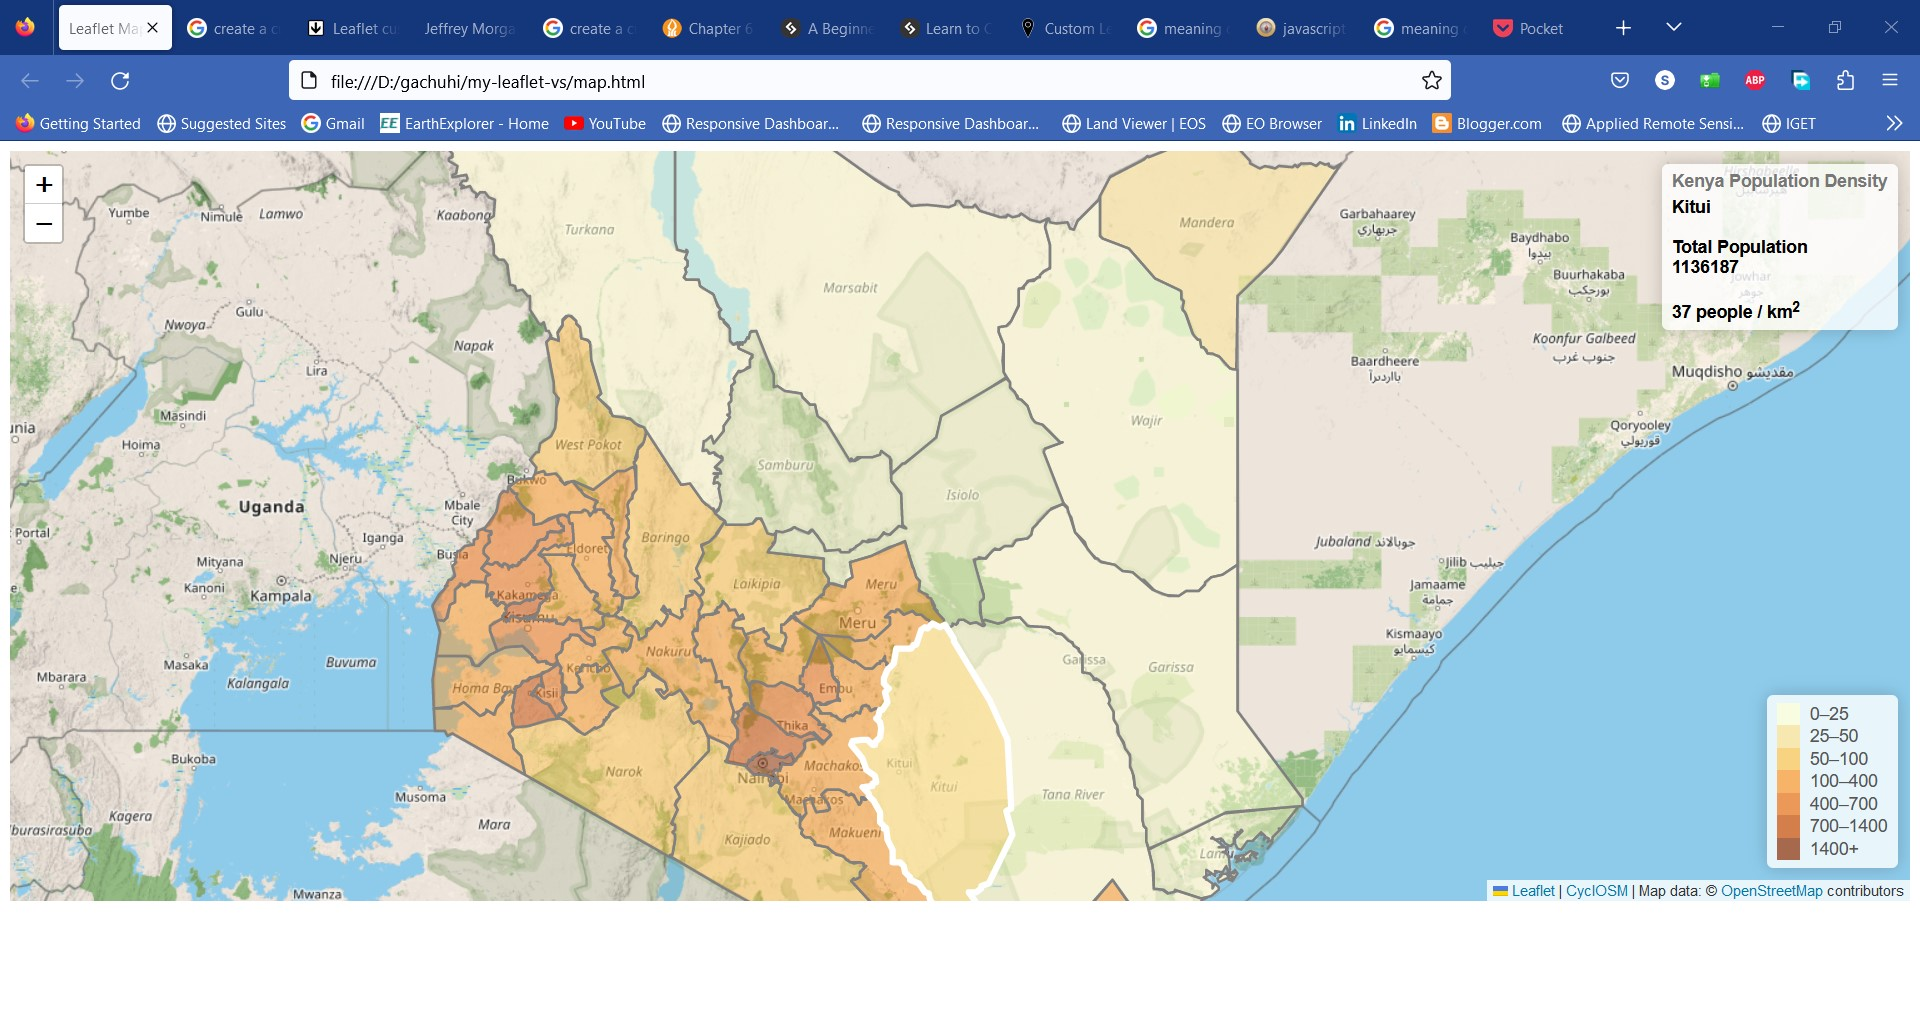
\includegraphics[width=26.67in]{../images/choropleth-legend}

The full code files are available from \href{https://www.dropbox.com/scl/fo/d8cwl9t1ay144vvy73pq6/h?dl=0\&rlkey=mardh4rwlqegfvf0vupbj0c28}{here}.

When creating choropleth maps, aim for challenging, impacting rather than merely informing.

\hypertarget{layer-groups-and-controls}{%
\chapter{Layer groups and controls}\label{layer-groups-and-controls}}

\hypertarget{purpose-of-layer-groups-and-controls}{%
\section{Purpose of layer groups and controls}\label{purpose-of-layer-groups-and-controls}}

Sometimes, one may wish their webmap to consist of several baselayers or overlay maps. This not only add, counter, or enhance the information provided, but they also allow additional interactive features apart from the usual clicking, dragging and zooming. Suppose you want your leaflet to have two basemap layers, with the option of switching to either, and same case to overlays, how would you proceed?

\hypertarget{set-up-the-basemaps}{%
\section{Set up the basemaps}\label{set-up-the-basemaps}}

In order to create controls, we have to set the variables in JavaScript Objects. Thereafter, the \texttt{L.controls.layers} class is used to parse the object values to the Leaflet map and show a UI control. To demonstrate this, open a new JavaScript file and name it \texttt{groups\_controls.js}. Insert the following code which will save our basemaps to the respective variables of \texttt{osm} and \texttt{cyclOSM}.

\begin{verbatim}
var osm = L.tileLayer('https://tile.openstreetmap.org/{z}/{x}/{y}.png', {
    maxZoom: 19,
    attribution: '&copy; <a href="http://www.openstreetmap.org/copyright">OpenStreetMap</a>'
});

var cyclOSM = L.tileLayer('https://{s}.tile-cyclosm.openstreetmap.fr/cyclosm/{z}/{x}/{y}.png', {
    maxZoom: 20,
    attribution: '<a href="https://github.com/cyclosm/cyclosm-cartocss-style/releases" title="CyclOSM - Open Bicycle render">CyclOSM</a> | Map data: &copy; <a href="https://www.openstreetmap.org/copyright">OpenStreetMap</a> contributors'
}); // the CyclOSM tile layer available from Leaflet servers
\end{verbatim}

We will pass the above two variables of \texttt{osm} and \texttt{cyclOSM} to the \texttt{L.map} class which has an option of \texttt{layers} in which one can parse the layers they wish to be displayed on the map.

\begin{verbatim}
var map = L.map('myMap', {
    layers: [osm, cyclOSM]
}).setView([-1.295287148, 36.81984753], 7);
\end{verbatim}

However, that will only add the first basemap variable that appears, that is of \texttt{osm} and blocking out that of \texttt{cylcOSM}. This is shown below.

\begin{Shaded}
\begin{Highlighting}[]
\NormalTok{knitr}\SpecialCharTok{::}\FunctionTok{include\_graphics}\NormalTok{(}\FunctionTok{rep}\NormalTok{(}\StringTok{\textquotesingle{}D:/gachuhi/my{-}leaflet/images/no{-}control.jpg\textquotesingle{}}\NormalTok{))}
\end{Highlighting}
\end{Shaded}

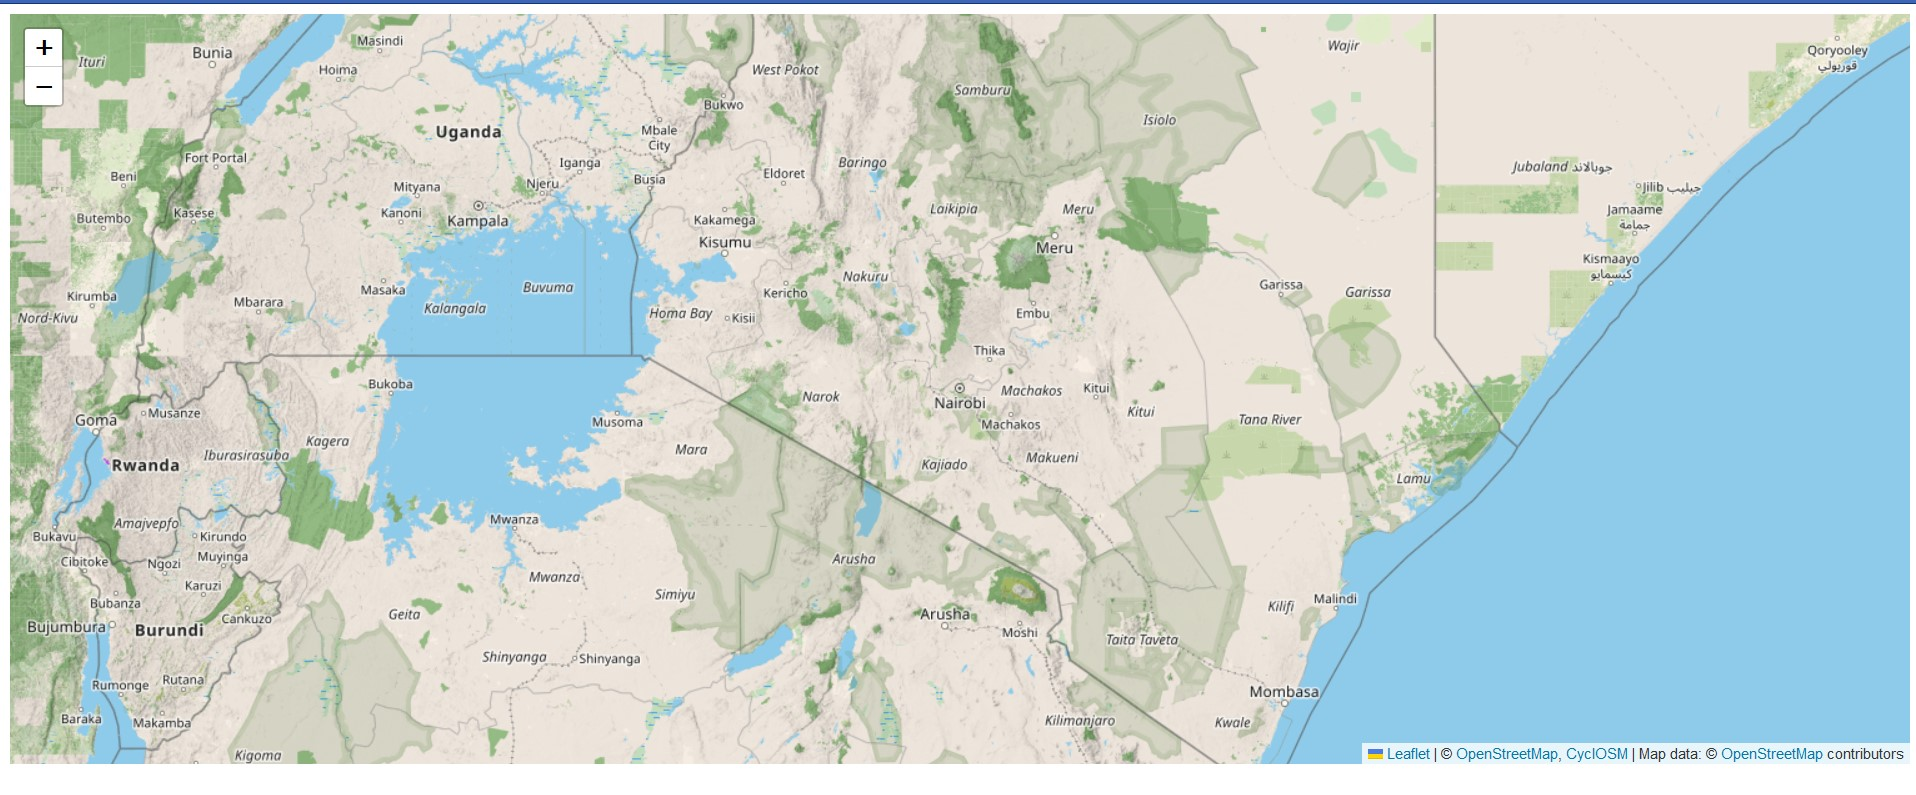
\includegraphics[width=26.61in]{../images/no-control}

\hypertarget{creating-the-controls}{%
\section{Creating the controls}\label{creating-the-controls}}

However, in order to give \texttt{cyclOSM} a fair chance, we need to store them in an object say \texttt{var\ basemaps} and parse it to \texttt{L.controls.layer} which shall create a checkbutton for each basemap. The below code does just that.

\begin{verbatim}
// Set object for the basemaps
var basemaps = {
    "OpenStreetMap": osm,
    'cycleOsm': cyclOSM,
}

L.control.layers(basemaps).addTo(map);

\end{verbatim}

This is what you get as a result.

\begin{Shaded}
\begin{Highlighting}[]
\NormalTok{knitr}\SpecialCharTok{::}\FunctionTok{include\_graphics}\NormalTok{(}\FunctionTok{rep}\NormalTok{(}\StringTok{\textquotesingle{}D:/gachuhi/my{-}leaflet/images/controls.jpg\textquotesingle{}}\NormalTok{))}
\end{Highlighting}
\end{Shaded}

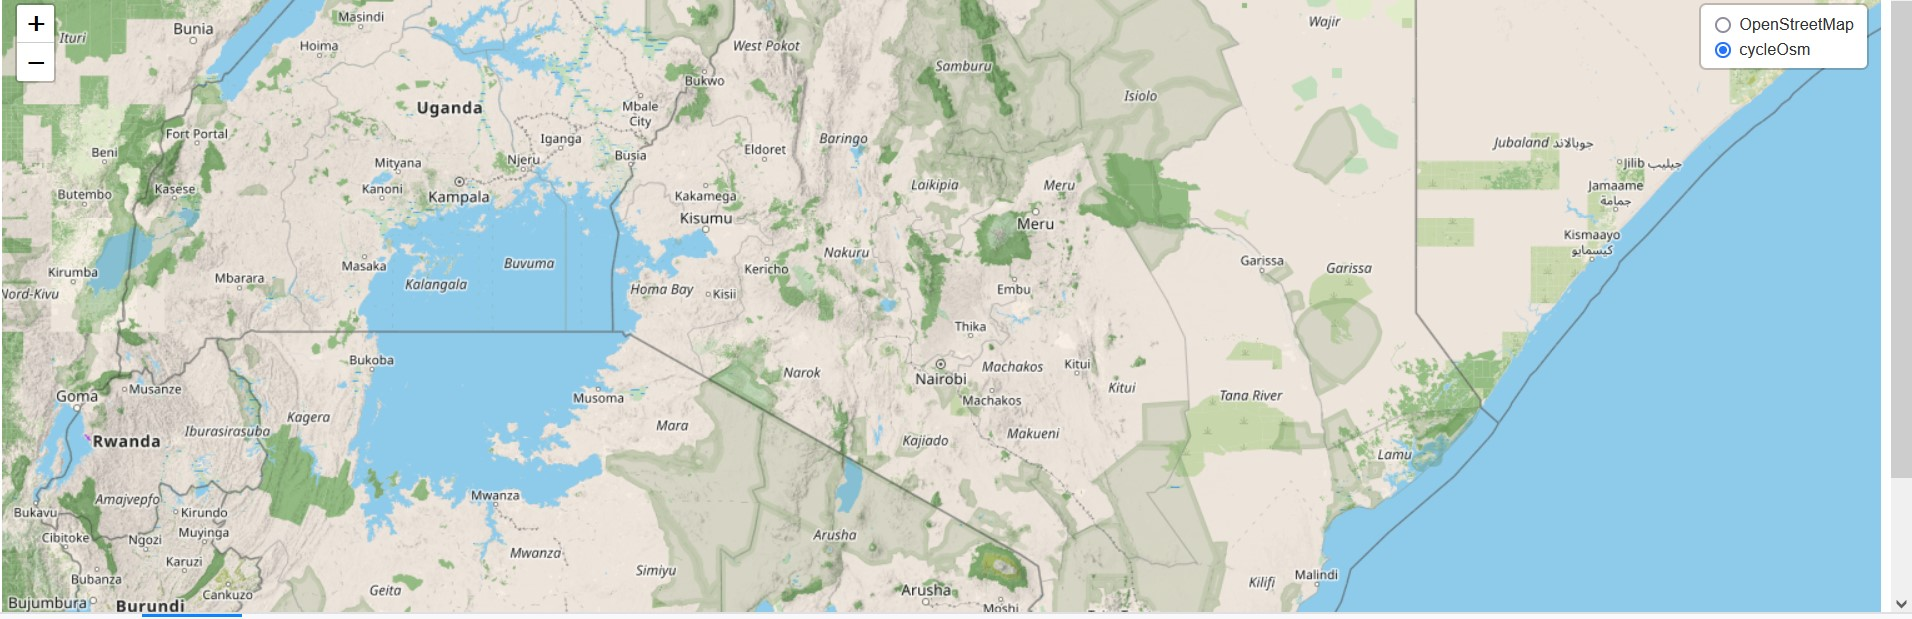
\includegraphics[width=26.56in]{../images/controls}

\hypertarget{adding-overlay-maps}{%
\section{Adding overlay maps}\label{adding-overlay-maps}}

Now we have seen how to add more than one basemap and make all of them appear in the layer control. As was the case for the \texttt{basemaps} variable, it can also be replicated for the overlay maps as well.

The first overlay we would like to create is a choropleth map display the percentage of conventional households with access to main sewers as per the \href{https://housingfinanceafrica.org/app/uploads/VOLUME-IV-KPHC-2019.pdf}{2019 census}. For simplicity purposes and to bypass errors we faced, we shall reuse the Ajax plugin for fetching GeoJSON files from online servers. As a reminder, we load Ajax into leaflet by insertint the following \texttt{\textless{}script\textgreater{}} tags into our \texttt{map.html}.

\begin{verbatim}
<script src="leaflet-ajax-gh-pages\dist\leaflet.ajax.js"></script>

<script src="leaflet-ajax-gh-pages\dist\leaflet.ajax.min.js"></script>
        <script src="leaflet-ajax-gh-pages\example\leaflet.spin.js"></script>
        <script src="leaflet-ajax-gh-pages\example\spin.js"></script> 
\end{verbatim}

I initially tried to load the json file for the sanitation overlay map layer using old \texttt{fetch} but the errors were too complex to solve. As they say, when life gives you bees, make honey, we decided to safely retreat to the young turk Ajax plugin. The following chunks of code will add the color function and styling for our countrywide sanitation map.

\begin{verbatim}
//// Adding some color
function getColor(d) {
    return d > 20 ? '#3288bd' :
            d > 10 ? '#99d594' :
            d > 6 ? '#e6f598' :
            d > 4 ? '#fee08b' :
            d >  2 ? '#fc8d59':
                     '#d53e4f';
                       
}

// Function for setting color (using arrow function)
var style = ((feature)=> {
    return {
        fillColor: getColor(feature.properties.Human_waste_disposal),
        weight: 2,
        opacity: 1,
        color: 'gray',
        fillOpacity: 0.9
    }
})
\end{verbatim}

Now let's add the overlay map that will display the accessibility to main sewer sanitation services. Spoiler alert: the statistics are grim.

\begin{verbatim}
// Adding the first overlay - map of household access to main sewer
var countySanitation = new L.geoJson.ajax("https://raw.githubusercontent.com/sammigachuhi/geojson_files/main/counties_sanitation.json", {
    style: style
})
.bindPopup(function (layer) {
            return `<b>County Name: </b> ${layer.feature.properties.ADM1_EN} <br>
            <b>Total County Population: </b><br> 
            ${layer.feature.properties.County_pop.toString()} <br><br>
            <b>% of Conventional Households with access to main sewer: </b><br><br>
            ${layer.feature.properties.Human_waste_disposal.toString()}`
        }).addTo(map);
\end{verbatim}

Let's add an accompanying legend for the above map. If you did the last \protect\hyperlink{creating-an-interactive-choropleth-map}{Chapter} of interactive choropleths, this should not be new.

\begin{verbatim}

// Create a legend
var legend = L.control({position: 'bottomright'});

legend.onAdd = function (map) {
    var div = L.DomUtil.create('div', 'info legend'),
    grades = [0, 2, 4, 6, 10, 20],
    labels = [];

    // loop through our density intervals and generate a label with a colored square for each interval
    for (var i = 0; i < grades.length; i++) {
        div.innerHTML += 
            '<i style="background:' + getColor(grades[i] + 1) + '"></i> ' + 
            grades[i] + (grades[i + 1] ? '&ndash;' + grades[i + 1] + '<br>' : '+');
    }
    return div;
}

legend.addTo(map);
\end{verbatim}

Just a stick and paste.

Now set an object to hold on of our two overlay maps. Don't worry, the second will come in no time.

\begin{verbatim}
var overlays = {
    'countySanitation': countySanitation,
}
\end{verbatim}

Finally parse it to the \texttt{L.controls.layer} class.

\begin{verbatim}
// Add layer controls
L.control.layers(basemaps, overlays).addTo(map);
\end{verbatim}

\begin{Shaded}
\begin{Highlighting}[]
\NormalTok{knitr}\SpecialCharTok{::}\FunctionTok{include\_graphics}\NormalTok{(}\FunctionTok{rep}\NormalTok{(}\StringTok{\textquotesingle{}D:/gachuhi/my{-}leaflet/images/controls{-}overlay.jpg\textquotesingle{}}\NormalTok{))}
\end{Highlighting}
\end{Shaded}

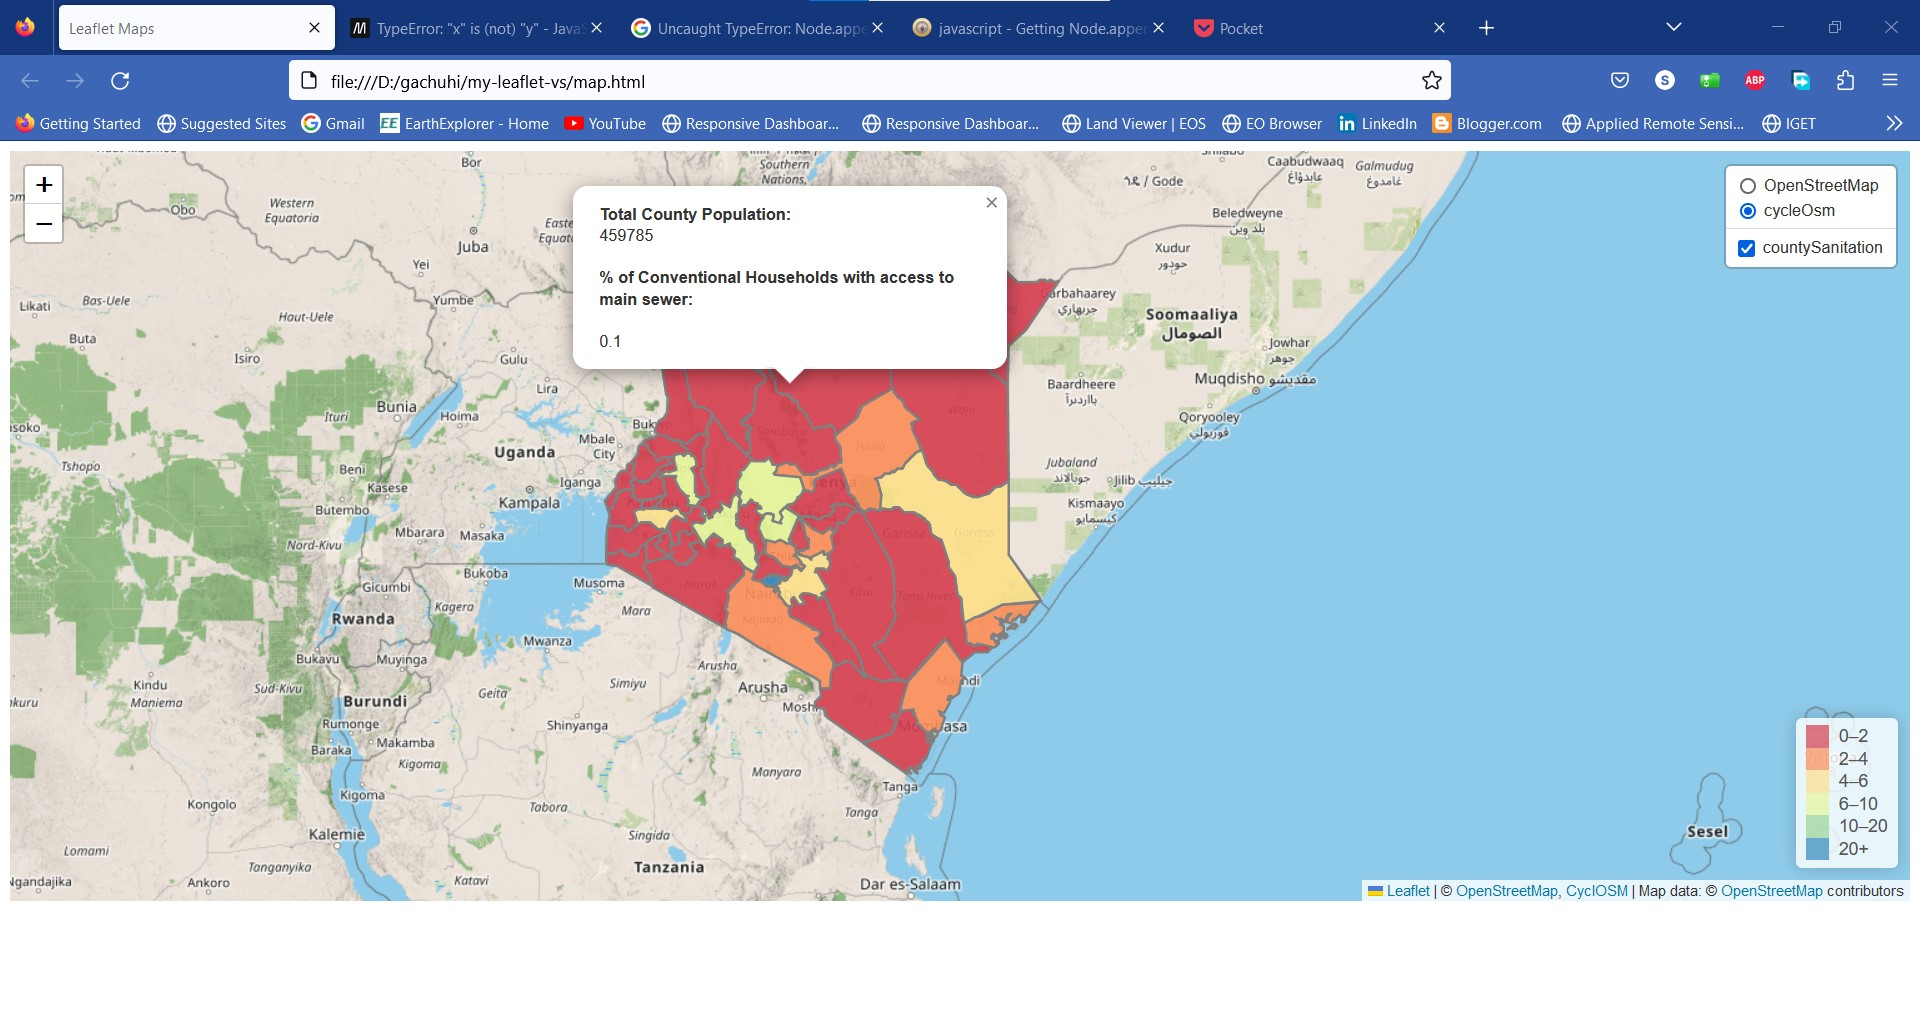
\includegraphics[width=26.67in]{../images/controls-overlay}

If you click anyone of the counties, you will see popups appear.

There is one more overaly we will add to our display to bring our experimentation with layer controls full circle. Remember the geojson of our \texttt{cities} variable? Let's call it to action again. Load the custom icon markers first that will differentiate the populations of our cities.

\begin{verbatim}
// Color icons
// Yellow Icon
var yellowIcon = new L.Icon({
    iconUrl: 'https://raw.githubusercontent.com/pointhi/leaflet-color-markers/master/img/marker-icon-2x-yellow.png',
    shadowUrl: 'https://cdnjs.cloudflare.com/ajax/libs/leaflet/0.7.7/images/marker-shadow.png',
    iconSize: [25, 41],
    iconAnchor: [12, 41],
    popupAnchor: [1, -34],
    shadowSize: [41, 41]
  });

// Orange Icon
var orangeIcon = new L.Icon({
    iconUrl: 'https://raw.githubusercontent.com/pointhi/leaflet-color-markers/master/img/marker-icon-2x-orange.png',
    shadowUrl: 'https://cdnjs.cloudflare.com/ajax/libs/leaflet/0.7.7/images/marker-shadow.png',
    iconSize: [25, 41],
    iconAnchor: [12, 41],
    popupAnchor: [1, -34],
    shadowSize: [41, 41]
  });

// Red Icon
var redIcon = new L.Icon({
    iconUrl: 'https://raw.githubusercontent.com/pointhi/leaflet-color-markers/master/img/marker-icon-2x-red.png',
    shadowUrl: 'https://cdnjs.cloudflare.com/ajax/libs/leaflet/0.7.7/images/marker-shadow.png',
    iconSize: [25, 41],
    iconAnchor: [12, 41],
    popupAnchor: [1, -34],
    shadowSize: [41, 41]
  });
\end{verbatim}

Let's load the \texttt{cities} geojson.

\begin{verbatim}
var cities = L.geoJson.ajax("https://raw.githubusercontent.com/sammigachuhi/geojson_files/main/cities-geojson2.geojson.txt", {
    pointToLayer: function (feature, latlng) {
            if (feature.properties.Population <= 250000) {
              return L.marker(latlng, {
                icon: yellowIcon 
              });
            } else if (feature.properties.Population <= 800000) {
              return L.marker(latlng, {
                icon: orangeIcon 
              });
            } else {
              return L.marker(latlng, {
                icon: redIcon 
              });
            }
            
          }
}).bindPopup(function (layer) {
      return `City: ${layer.feature.properties.City},<br>
      Population: ${layer.feature.properties.Population}`;
    }).addTo(map);
    
\end{verbatim}

Add the \texttt{cities} variable as one of the keys to our \texttt{overlays} variable and finally parse the overlays object to \texttt{L.control.layers}.

\begin{verbatim}
// Set object for the overlay maps
var overlays = {
    'countySanitation': countySanitation,
    'cities': cities
}

// Add layer controls
L.control.layers(basemaps, overlays).addTo(map);
\end{verbatim}

In the previous \protect\hyperlink{creating-an-interactive-choropleth-map}{chapter}, we ended by saying that we strive to make our choropleths map challenge, charge rather than merely informing. This seems a sketchy type, but it shows the discrepancy as well as the effort needed for Kenya to bring a centralized sanitation system to every household. Sanitation matters may always sound insensitive, but the true barometer of any civilization is its sanitation.

Finally, we tried playing around with the options available to the \texttt{L.controls.layer} including the simple one as changing position, but everytime a new option was provided in to the parenthesis, as in \texttt{L.control.layers(basemap,\ overlaymap,\ \{options\})}, the control would disappear.

\begin{Shaded}
\begin{Highlighting}[]
\NormalTok{knitr}\SpecialCharTok{::}\FunctionTok{include\_graphics}\NormalTok{(}\FunctionTok{rep}\NormalTok{(}\StringTok{\textquotesingle{}D:/gachuhi/my{-}leaflet/images/controls{-}all.jpg\textquotesingle{}}\NormalTok{))}
\end{Highlighting}
\end{Shaded}

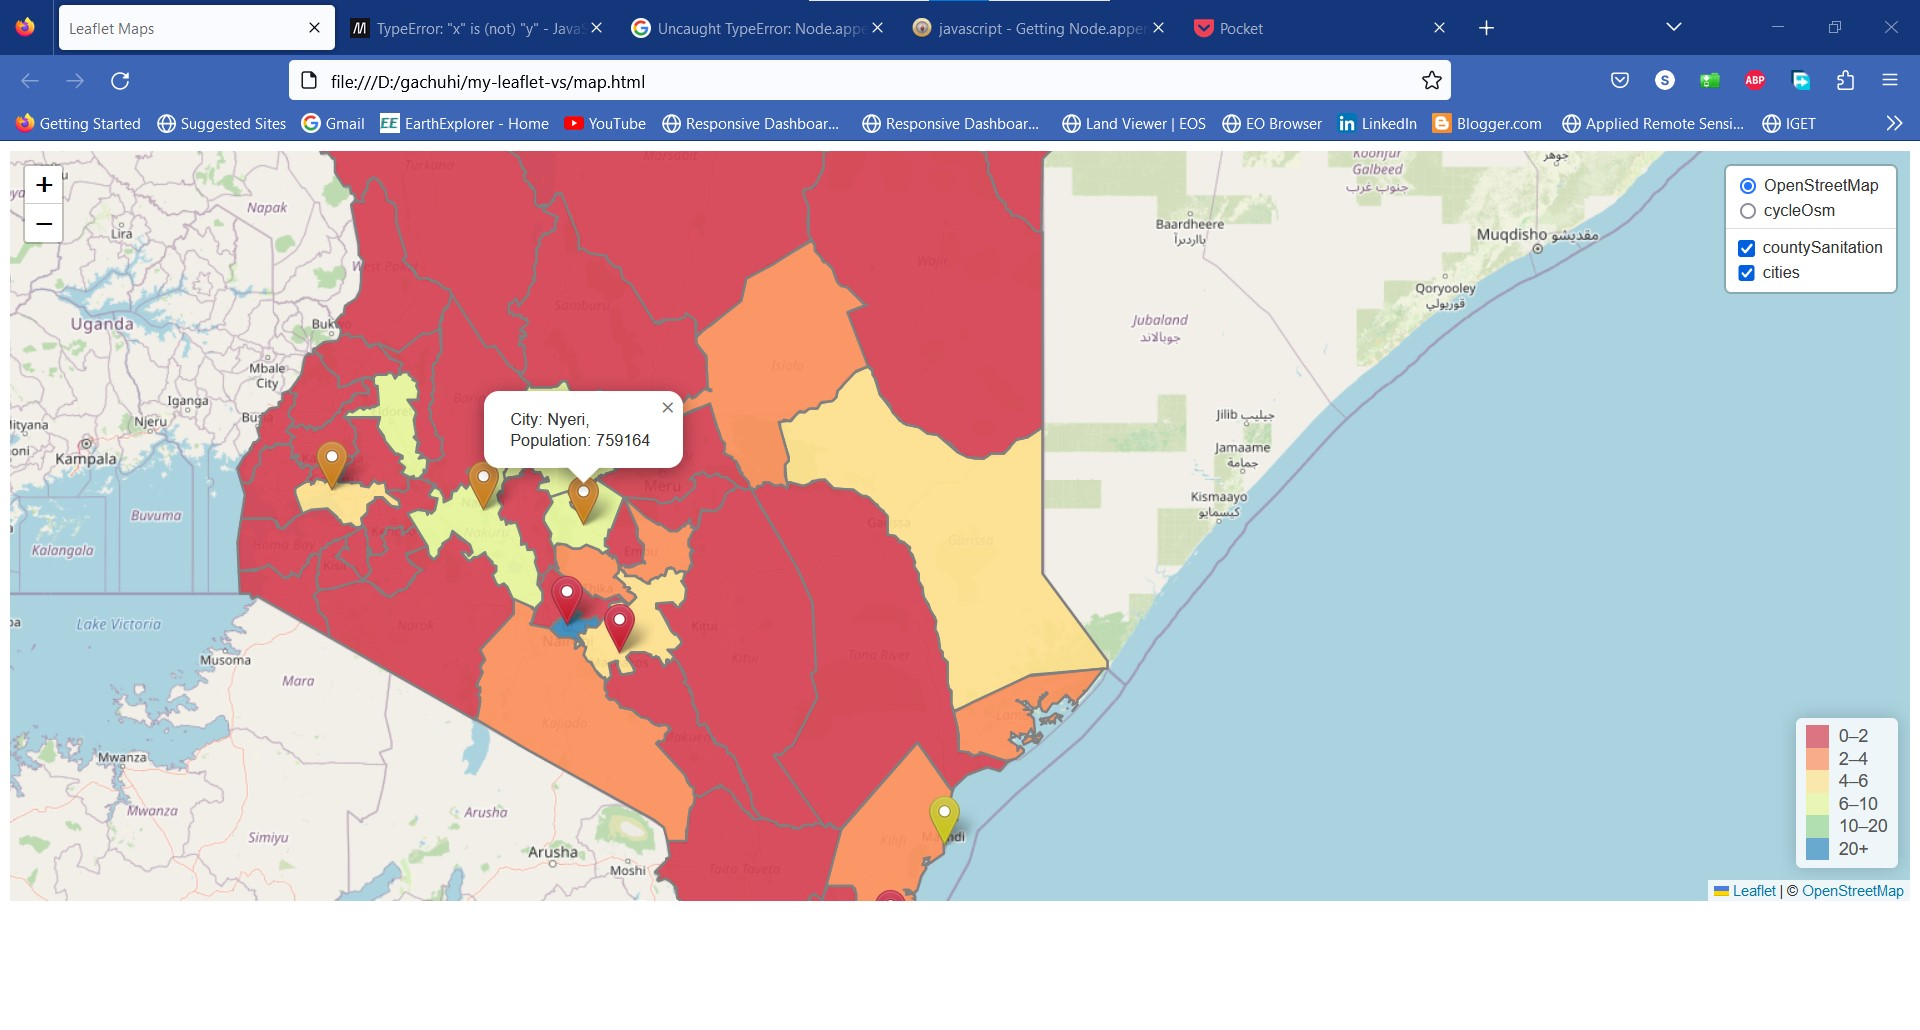
\includegraphics[width=26.67in]{../images/controls-all}

\hypertarget{add-a-scale-bar}{%
\section{Add a scale bar}\label{add-a-scale-bar}}

Adding a small reactive scale with an option to demonstrate will not hurt!

\begin{verbatim}
// Add scale
L.control.scale({position:'bottomleft'}).addTo(map);
\end{verbatim}

\begin{Shaded}
\begin{Highlighting}[]
\NormalTok{knitr}\SpecialCharTok{::}\FunctionTok{include\_graphics}\NormalTok{(}\FunctionTok{rep}\NormalTok{(}\StringTok{\textquotesingle{}D:/gachuhi/my{-}leaflet/images/controls{-}scale.jpg\textquotesingle{}}\NormalTok{))}
\end{Highlighting}
\end{Shaded}

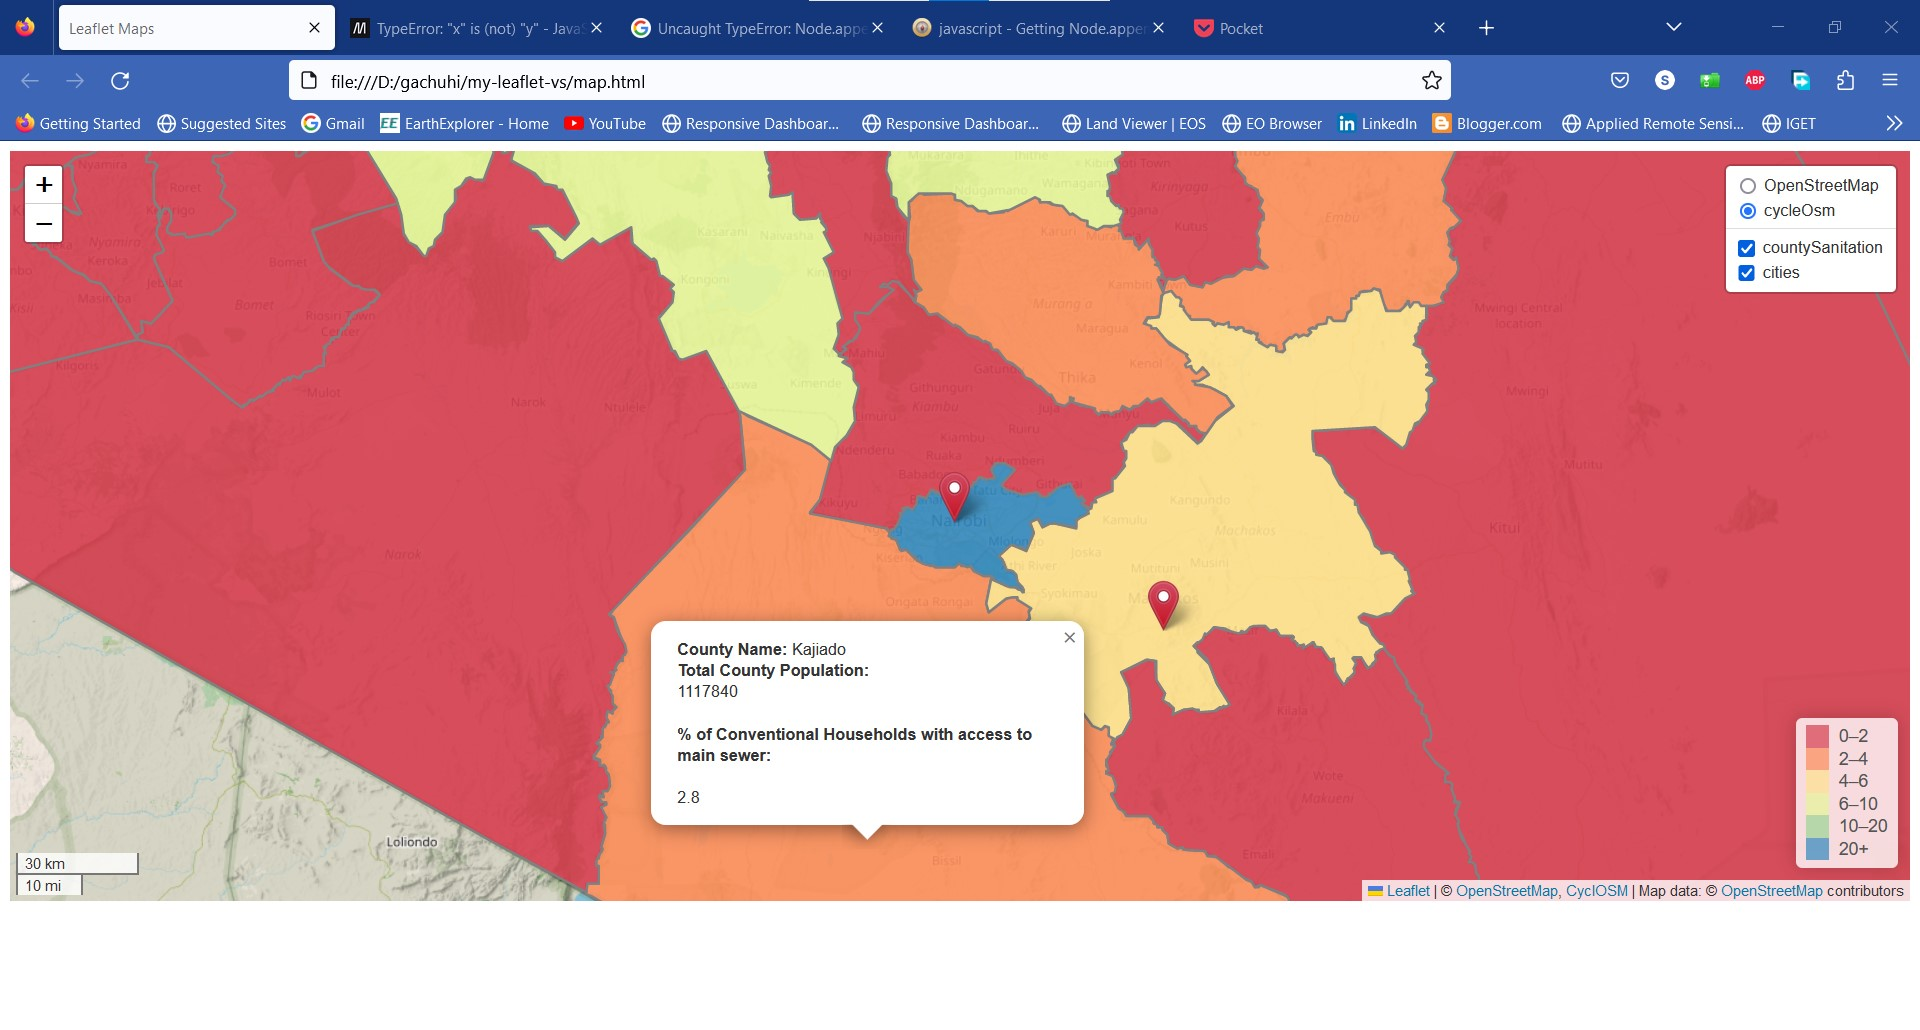
\includegraphics[width=26.67in]{../images/controls-scale}

All the files and scripts used in this chapter can be accessed \href{https://www.dropbox.com/scl/fo/0njhl757vantwggnsidks/h?dl=0\&rlkey=18m27j58agq6209lkppkdtgqo}{here}.

\hypertarget{heatmaps}{%
\chapter{Heatmaps}\label{heatmaps}}

\hypertarget{what-are-heatmaps}{%
\section{What are heatmaps?}\label{what-are-heatmaps}}

\href{https://www.gislounge.com/heat-maps-in-gis/}{Heatmaps} are a type of maps that geographically visualize locations with patterns of higher than average occurrence of particular variables say crime, disease, service centres and et cetera.

\hypertarget{loading-the-heatmap-plugin}{%
\section{Loading the heatmap plugin}\label{loading-the-heatmap-plugin}}

A tool for drawing heatmaps does not come prepackaged in leaflet. We therefore have to use an external plugin by the name of \href{https://github.com/Leaflet/Leaflet.heat}{Leaflet.heat}. Yours truly downloaded it from the site hyperlinked in the aforementioned sentence. In case you missed it, the link is \href{https://codeload.github.com/Leaflet/Leaflet.heat/zip/refs/heads/gh-pages}{here}. Download and extract the folder in the same directory as your \texttt{map.html}.

Once you have extracted, open your \texttt{map.html} and add another \texttt{\textless{}script\textgreater{}} tag within your \texttt{\textless{}head\textgreater{}} element.

\begin{verbatim}
<script src="Leaflet.heat-gh-pages\Leaflet.heat-gh-pages\dist\leaflet-heat.js"></script>
\end{verbatim}

Thereafter, we will have to think of a way of loading the GeoJson to our \texttt{heatmap.js} file, which we shall use as the JavaScript file for our heatmap code. You may thin of using \texttt{fetch} or \texttt{L.geoJson.ajax} for this purpose but not so fast. Yours truly tried all the above and even though they are proven ways of loading a JavaScript file as we have seen so far it didn't work in creating a heatmap. This is even when we stored the \texttt{fetch} and \texttt{L.geoJson.ajax} functions into variables to pass them to \texttt{L.heatLayer}. \texttt{L.heatLayer} is a function that is made possible from the Leaflet.heat plugin we parsed into \texttt{map.html} above.

So, what method works in creating a heatmap?

After much internet searching, I came across a code in Stack Overflow. However, it only works after inserting another Ajax plugin. Luckily no download is needed so insert this new \texttt{\textless{}script\textgreater{}} into your \texttt{map.html}.

\begin{verbatim}
<script src="https://ajax.googleapis.com/ajax/libs/jquery/2.1.4/jquery.min.js"></script>
\end{verbatim}

\hypertarget{creating-the-leaflet-heatmap}{%
\section{Creating the Leaflet heatmap}\label{creating-the-leaflet-heatmap}}

Let's call the usual suspects of adding a basemap.

\begin{verbatim}
var map = L.map('myMap').setView([0.3556, 37.5833], 6.5);

L.tileLayer('https://tile.openstreetmap.org/{z}/{x}/{y}.png', {
    attribution: '&copy; <a href="https://www.openstreetmap.org/copyright">OpenStreetMap</a> contributors'
}).addTo(map);
\end{verbatim}

Thereafter, we add the following large code chunks.

\begin{verbatim}
var geoJsonUrl = "https://raw.githubusercontent.com/sammigachuhi/geojson_files/main/selected_hospitals.json"

    var geojsonLayer = $.ajax({
    url : geoJsonUrl,
    dataType : 'json',
    jsonpCallback: 'getJson',
    success : console.log("Data successfully loaded!"),
    });

geoJson2heat = ((geojson) => {
        return geojson.features.map(function(feature) {
        return [parseFloat(feature.geometry.coordinates[1]), 
                parseFloat(feature.geometry.coordinates[0])];
        });
        });


$.when(geojsonLayer).done(function() {
        // var kill = L.geoJSON(geojsonLayer.responseJSON);
        var layer = geoJson2heat(geojsonLayer.responseJSON, 4);
        var heatMap = L.heatLayer(layer, { 
                radius: 40,
                blur: 10, 
                gradient: {
                        '0': 'Navy', '0.25': 'Navy',
                        '0.26': 'Green',
                        '0.5': 'Green',
                        '0.51': 'Yellow',
                        '0.75': 'Yellow',
                        '0.76': 'Red',
                        '1': 'Red'
                      },
                maxZoom: 13});
        map.addLayer(heatMap);
        });
\end{verbatim}

To give credit where it is due, the code chunks were taken from \href{https://gis.stackexchange.com/questions/337294/heatmap-with-geojson-leaflet-and-leaflet-heat-plugin?utm_source=pocket_reader}{this Stack Overflow question} and modified a bit.

I will do everyone justice by going through the preceding code bit by bit.

\begin{verbatim}
var geoJsonUrl = "https://raw.githubusercontent.com/sammigachuhi/geojson_files/main/selected_hospitals.json"

    var geojsonLayer = $.ajax({
    url : geoJsonUrl,
    dataType : 'json',
    jsonpCallback: 'getJson',
    success : console.log("Data successfully loaded!"),
    });

\end{verbatim}

The \texttt{var\ geoJsonUrl} gets the link to our hospitals json file. The \texttt{var\ geojsonLayer} uses the Asynchronous Javascript And Xml (Ajax) method to load data from our Github server. If successfull, we get the message ``Data successfully loaded!'' in our browser console.

\begin{verbatim}
geoJson2heat = ((geojson) => {
        return geojson.features.map(function(feature) {
        return [parseFloat(feature.geometry.coordinates[1]), 
                parseFloat(feature.geometry.coordinates[0])];
        });
        });
        
\end{verbatim}

The above code chunk is fairly easy to understand. The function passed to \texttt{geoJson2heat} uses the \texttt{map} method to iterate over every element, such as cities in the json file and retrieve the longitude and latitude coordinates. Notice the format has been inverted. Rathater than {[}0{]}\ldots{} {[}1{]} for Lat-Lon, we use {[}1{]}\ldots{[}0{]}.

The final is a jQuery function that will return the heatmap layer.

\begin{verbatim}
$.when(geojsonLayer).done(function() {
        // var kill = L.geoJSON(geojsonLayer.responseJSON);
        var layer = geoJson2heat(geojsonLayer.responseJSON, 4);
        var heatMap = L.heatLayer(layer, { 
                radius: 40,
                blur: 10, 
                gradient: {
                        '0': 'Navy', '0.25': 'Navy',
                        '0.26': 'Green',
                        '0.5': 'Green',
                        '0.51': 'Yellow',
                        '0.75': 'Yellow',
                        '0.76': 'Red',
                        '1': 'Red'
                      },
                maxZoom: 13});
        map.addLayer(heatMap);
        });
\end{verbatim}

Honestly the last was a bit of a stretch as yours truly is yet to encounter use of jQuery that much nowadays.

\begin{Shaded}
\begin{Highlighting}[]
\NormalTok{knitr}\SpecialCharTok{::}\FunctionTok{include\_graphics}\NormalTok{(}\FunctionTok{rep}\NormalTok{(}\StringTok{\textquotesingle{}D:/gachuhi/my{-}leaflet/images/heatmap.jpg\textquotesingle{}}\NormalTok{))}
\end{Highlighting}
\end{Shaded}

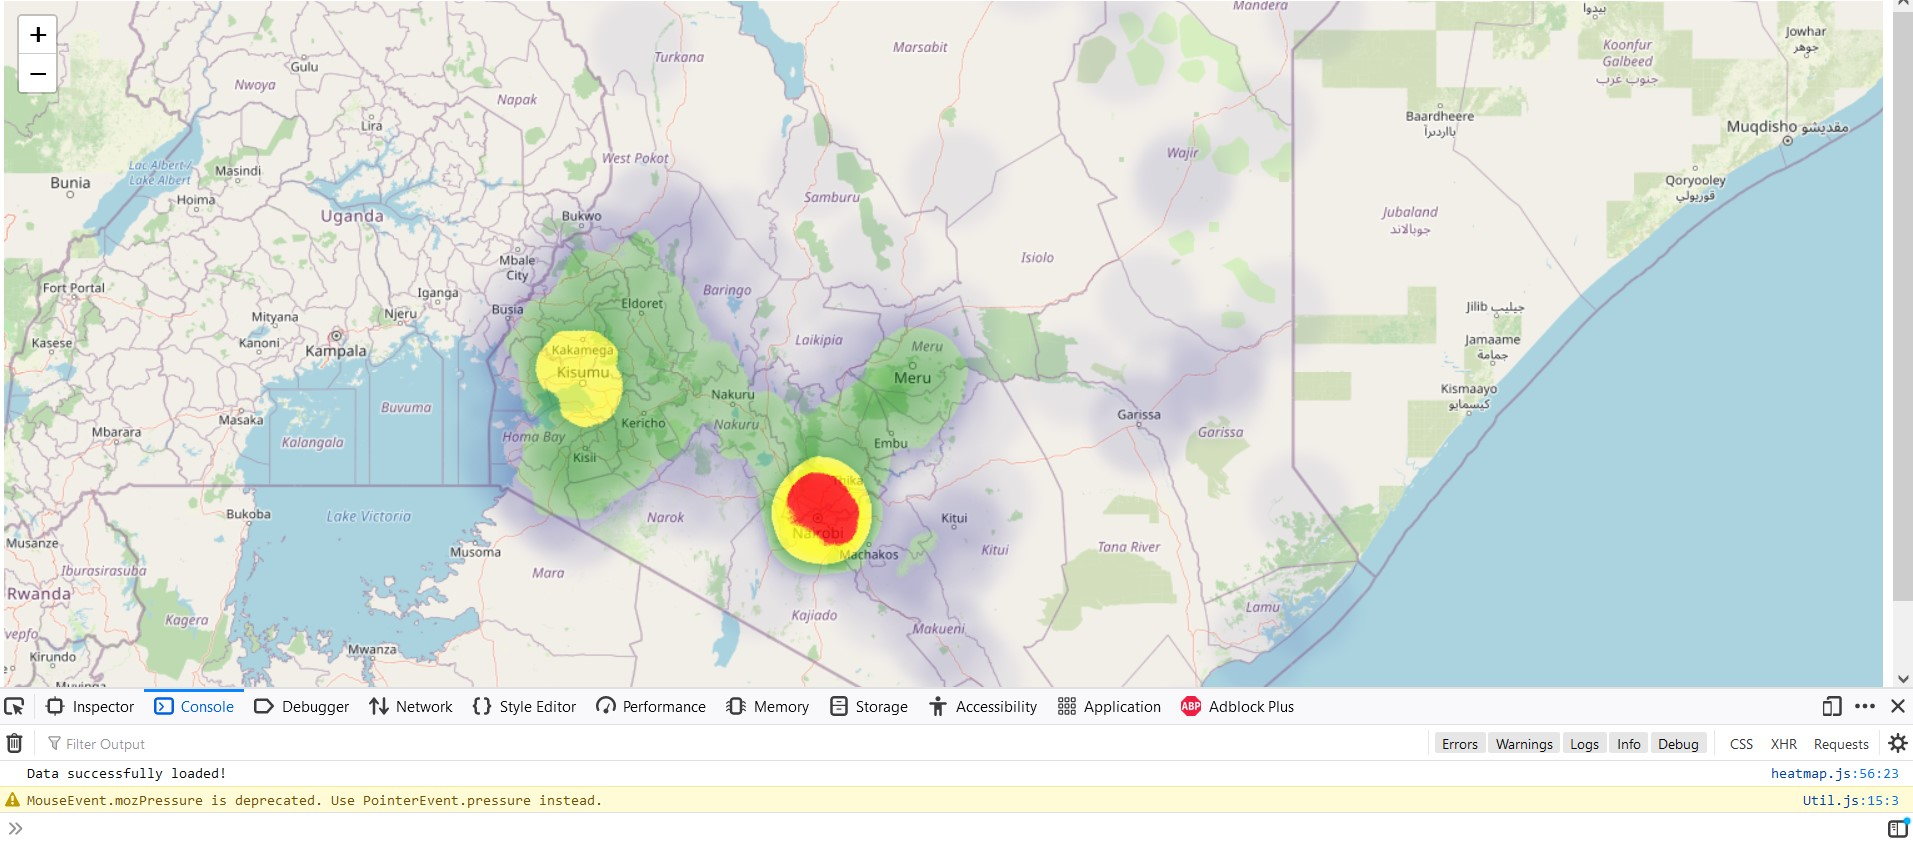
\includegraphics[width=26.57in]{../images/heatmap}

The full code files are available from \href{https://www.dropbox.com/scl/fo/cgfftdcw8u7lqyqfu38gu/h?dl=0\&rlkey=7ywjiud4vo24llrx192rvgf4d}{here}.

\hypertarget{cluster-to-reduce-the-clutter}{%
\chapter{Cluster to reduce the clutter}\label{cluster-to-reduce-the-clutter}}

\hypertarget{a-map-full-of-clutter}{%
\section{A map full of clutter}\label{a-map-full-of-clutter}}

There comes a time when it is convenient to coalesce several points into single multi-cluster point. Consider the following example: you have a geojson file with over 10000 points of houses within a densely populated region, say an island of 5km by 5km, if by any chance such a scenario exists. Will you want to display such a gigantic number of points within such a small area? That would be an overkill! Moreover, it will seem incomprehensible to the viewer. Consider the following example we set up in a new JavaScript file which we fondly called \texttt{cluster-markers.js}.

\begin{verbatim}
var map = L.map('myMap').setView([-1.295287148, 36.81984753], 7);

L.tileLayer('https://tile.openstreetmap.org/{z}/{x}/{y}.png', {
    maxZoom: 19,
    attribution: '&copy; <a href="http://www.openstreetmap.org/copyright">OpenStreetMap</a>'
}).addTo(map);


url = 'https://raw.githubusercontent.com/sammigachuhi/geojson_files/main/selected_hospitals.json'

L.geoJson.ajax(url).addTo(map);

var markers = L.markerClusterGroup();
\end{verbatim}

The following is the result we got.

\begin{Shaded}
\begin{Highlighting}[]
\NormalTok{knitr}\SpecialCharTok{::}\FunctionTok{include\_graphics}\NormalTok{(}\FunctionTok{rep}\NormalTok{(}\StringTok{\textquotesingle{}D:/gachuhi/my{-}leaflet/images/clutter{-}points.jpg\textquotesingle{}}\NormalTok{))}
\end{Highlighting}
\end{Shaded}

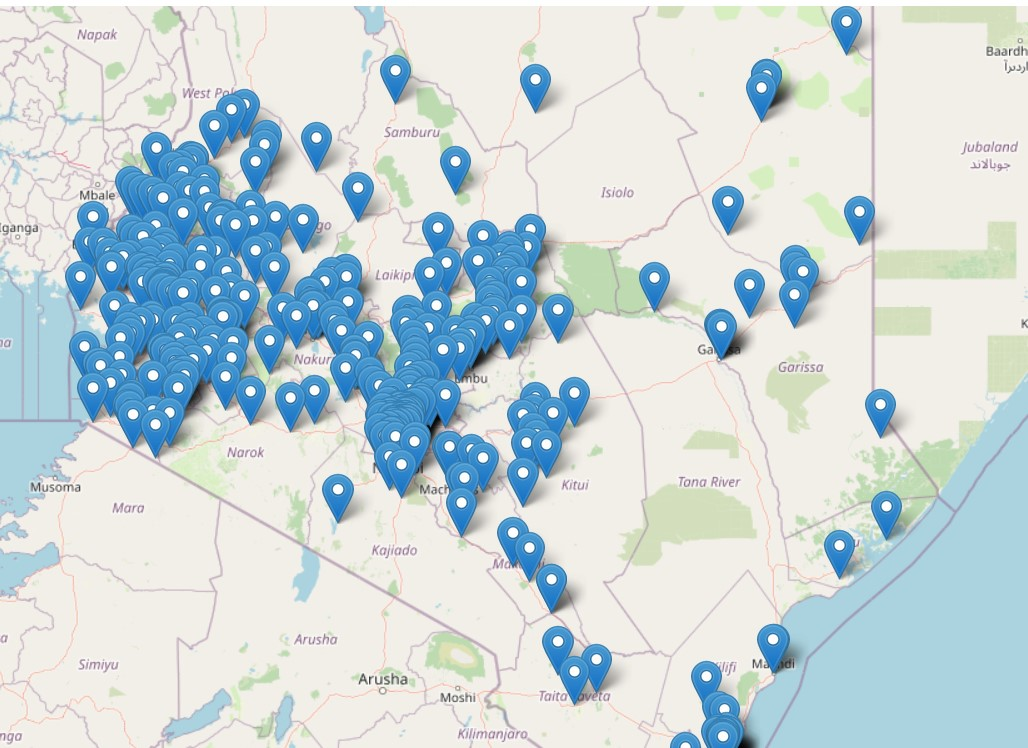
\includegraphics[width=14.28in]{../images/clutter-points}

Not good at all. The \texttt{Leaflet.markercluster} plugin is what transforms a clutter map into one of neatly arranged clustered marker points.

\hypertarget{preparations}{%
\section{Preparations}\label{preparations}}

Creating a cluster marker map is fairly easy. You will first have to insert the \texttt{Leaflet.markerCluster} plugin into \texttt{map.html}. The plugin is available from \href{https://github.com/Leaflet/Leaflet.markercluster/archive/refs/heads/master.zip}{here}. Insert the following \texttt{\textless{}script\textgreater{}} tag into the \texttt{\textless{}head\textgreater{}} element of your \texttt{map.html}.

\begin{verbatim}
<script src="Leaflet.markercluster-1.4.1\Leaflet.markercluster-1.4.1\dist\leaflet.markercluster.js"></script>
\end{verbatim}

You will also have to insert the \texttt{Leaflet.markercluster} CSS properties via the \texttt{\textless{}link\textgreater{}} tag too. Add the following \texttt{\textless{}link\textgreater{}} tag for \texttt{Leaflet.markercluster} after the other \texttt{\textless{}link\textgreater{}} properties.

\begin{verbatim}
<link rel="stylesheet" href="Leaflet.markercluster-master\Leaflet.markercluster-master\dist\MarkerCluster.Default.css"> 
\end{verbatim}

Don't underestimate them. These CSS properties are necessary to style your cluster points in a nice way -to make it easy on the eye.

Hope you also referenced your \texttt{map.html} to the \texttt{cluster-markers.js} in the \texttt{\textless{}script\textgreater{}} file inside the \texttt{\textless{}body\textgreater{}} element!

If you had done the small exercise at the beginning of the chapter, the following code should be present.

\begin{verbatim}
var map = L.map('myMap').setView([-1.295287148, 36.81984753], 7);

L.tileLayer('https://tile.openstreetmap.org/{z}/{x}/{y}.png', {
    maxZoom: 19,
    attribution: '&copy; <a href="http://www.openstreetmap.org/copyright">OpenStreetMap</a>'
}).addTo(map);


url = 'https://raw.githubusercontent.com/sammigachuhi/geojson_files/main/selected_hospitals.json'
\end{verbatim}

\hypertarget{behold-a-cluster-marker-map}{%
\section{Behold, a cluster marker map!}\label{behold-a-cluster-marker-map}}

Delete the \texttt{L.geoJson.ajax(url).addTo(map);}, we won't need it now. Our real work of creating a cluster marker map begins with the \texttt{markerClusterGroup}. Let's proceed!

\begin{verbatim}
var markers = L.markerClusterGroup();
\end{verbatim}

We shall use Ajax again but this time round we shall pass in some functions to customize the appearance and functionalities of our GeoJson markers.

\begin{verbatim}

L.geoJson.ajax(url, {
    pointToLayer: ((feature, latLng) => {
        return markers.addLayer(L.circleMarker(latLng));
    }),

    onEachFeature: ((feature, layer) => {
        layer.bindPopup(`<b>Facility Name:</b> ${feature.properties.Facility_N} <br>
        <b>Type:</b> ${feature.properties.Type}`)
    })
}).addTo(map);
\end{verbatim}

Remember \texttt{pointToLayer}? It defines how the GeoJson file will appear. The \texttt{pointToLayer} retrieves the Latitude-Longitude coordinates, creates circle markers out of them before finally parsing to the \texttt{markers} variable in the return keyword.

How about for \texttt{onEachFeature}. You can guess. \emph{O}n \emph{E}ach \emph{F}eature, do this and that. In our case we bind a popup of facility name and type which will appear when a circle marker is clicked on.

Actually, the above code sort of finished the work for us.

\begin{Shaded}
\begin{Highlighting}[]
\NormalTok{knitr}\SpecialCharTok{::}\FunctionTok{include\_graphics}\NormalTok{(}\FunctionTok{rep}\NormalTok{(}\StringTok{\textquotesingle{}D:/gachuhi/my{-}leaflet/images/cluster{-}marker{-}map.jpg\textquotesingle{}}\NormalTok{))}
\end{Highlighting}
\end{Shaded}

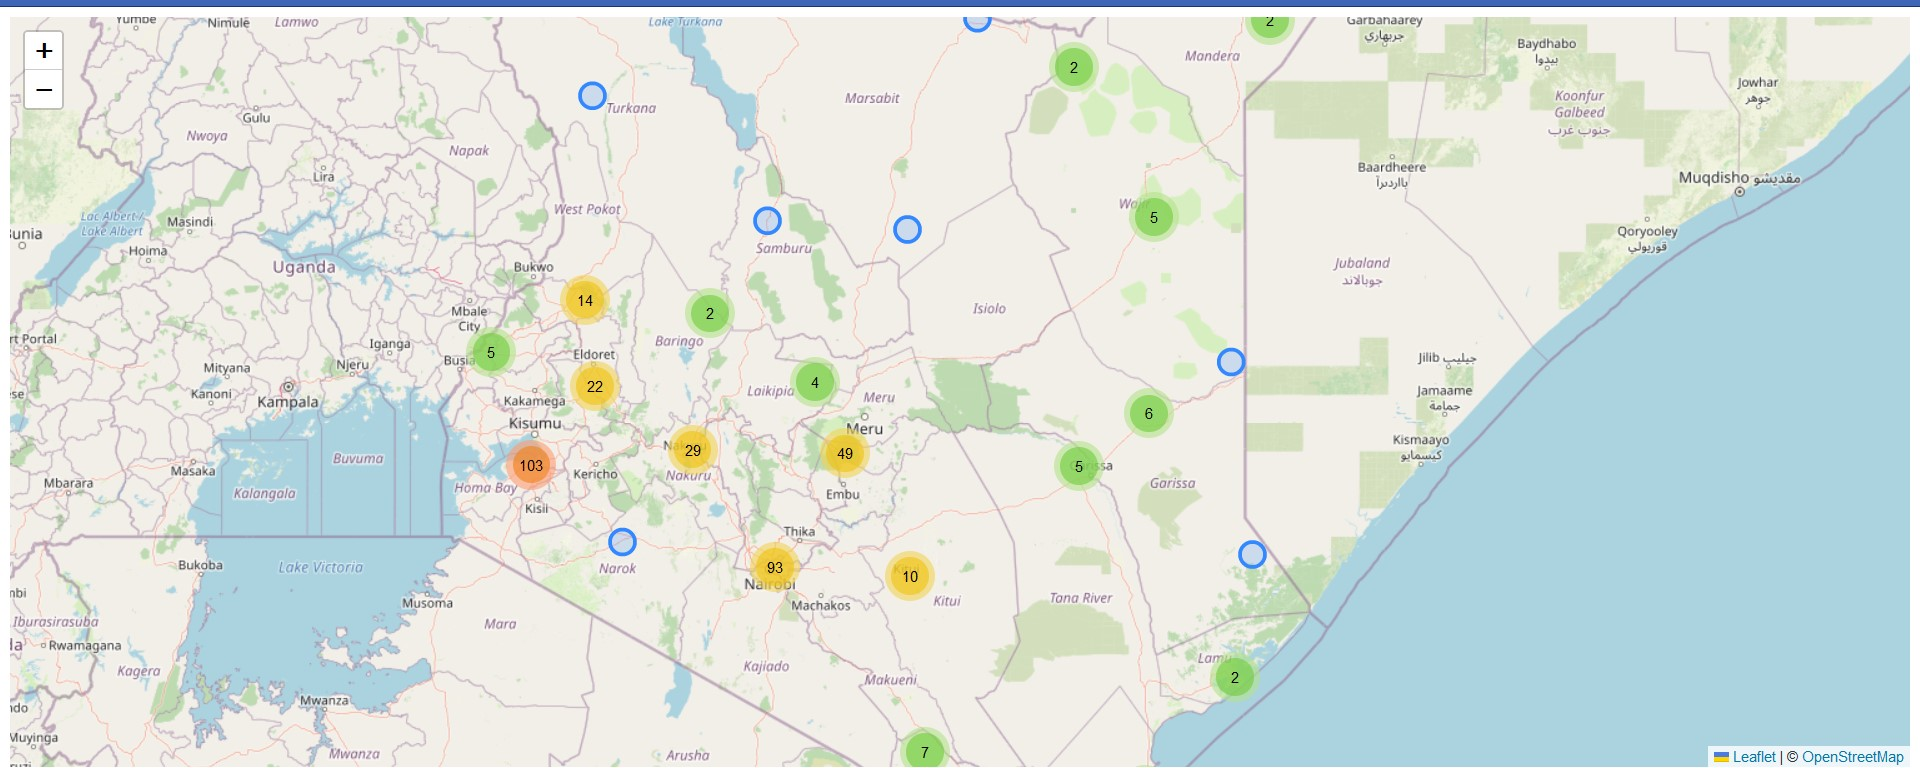
\includegraphics[width=26.67in]{../images/cluster-marker-map}

Zoom in and out and watch the circle markers \emph{spidefy} to individual points with a popup. I have restrained from tweaking because the defaults are already good enough. See them from this \href{https://github.com/Leaflet/Leaflet.markercluster}{Github Page}.

However, as good practice, we need to add the \texttt{markers} global variable to the map. We do so by using the following code.

\begin{verbatim}
map.addLayer(markers)
\end{verbatim}

\texttt{addLayers}, just like the name suggests, adds the given layer to the map.

The \texttt{L.circleMarker} in the \texttt{pointToLayer} key of the ajax function can be replaced with \texttt{L.marker()}. However, lone hospitals especially to the northeast of Kenya, and when clusters are specified to their individual points will resort to the default marker style of Leaflet. Below is how they would look, and is far from aesthetic.

\begin{Shaded}
\begin{Highlighting}[]
\NormalTok{knitr}\SpecialCharTok{::}\FunctionTok{include\_graphics}\NormalTok{(}\FunctionTok{rep}\NormalTok{(}\StringTok{\textquotesingle{}D:/gachuhi/my{-}leaflet/images/cluster{-}marker{-}plain.jpg\textquotesingle{}}\NormalTok{))}
\end{Highlighting}
\end{Shaded}

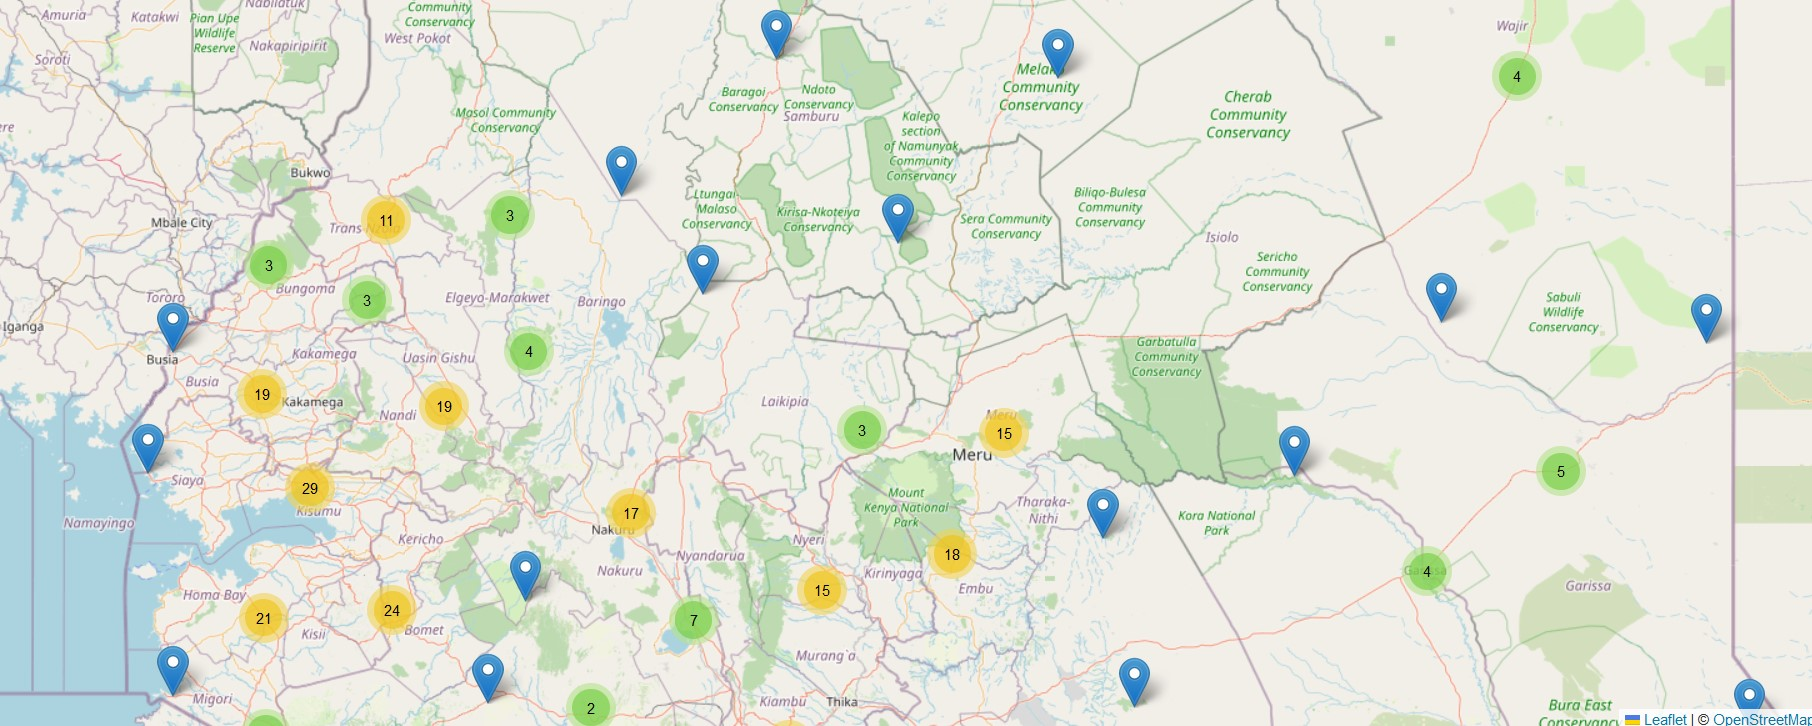
\includegraphics[width=25.17in]{../images/cluster-marker-plain}

Coming back full circle, circle markers are way better.

Most of the ajax code was inspired by this \href{https://www.youtube.com/watch?v=R-V7XFUbrkw\&t=625s}{video}.

But wait! Hold your horses, there is a bug. Try to click on any of the spiderfied or lone hospitals and you will notice something that will raise eyebrows. All hospitals display the following popup when clicked:

\begin{verbatim}
Facility Name: Wajir Tb Manyatta Sub - District Hospital
Type: Sub-District Hospital
\end{verbatim}

\begin{Shaded}
\begin{Highlighting}[]
\NormalTok{knitr}\SpecialCharTok{::}\FunctionTok{include\_graphics}\NormalTok{(}\FunctionTok{rep}\NormalTok{(}\StringTok{\textquotesingle{}D:/gachuhi/my{-}leaflet/images/cluster{-}marker{-}bug.jpg\textquotesingle{}}\NormalTok{))}
\end{Highlighting}
\end{Shaded}

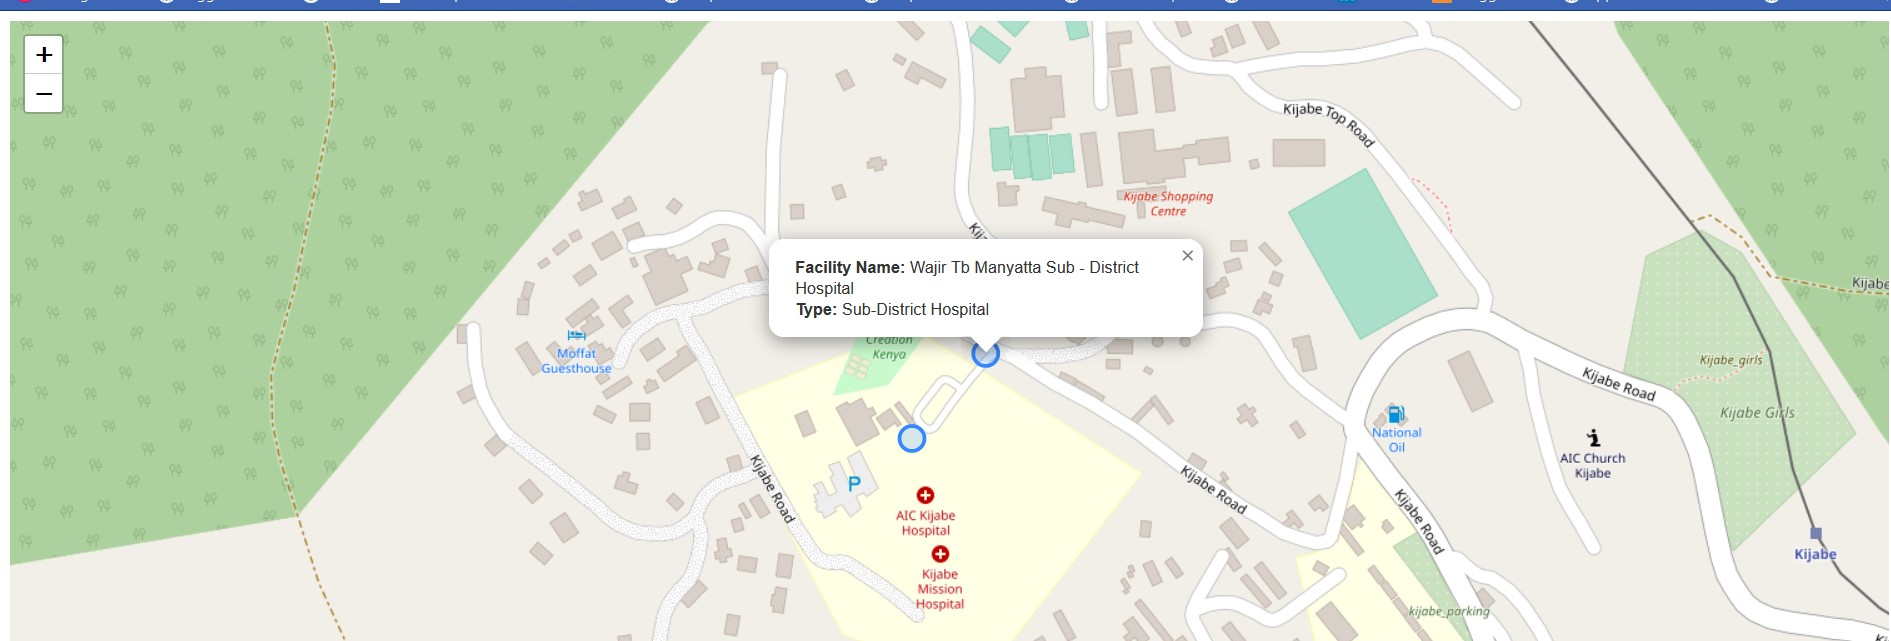
\includegraphics[width=26.26in]{../images/cluster-marker-bug}

Unless a developer would like to be left with an egg on the face for assigning wrong place names, this should be dealt with expeditiously. Our code is alright, since it works in other scenarios such as \href{https://gis.stackexchange.com/questions/346104/popup-with-leaflet-markercluster-in-leaflet-map?utm_source=pocket_reader}{here}. Yours truly suspects that the Ajax plugin is the issue, since \texttt{L.geoJSON} works perfectly in displaying the correct popup for each hospital.

Time to try a different strategy: using \texttt{fetch} API. At least \texttt{fetch} will use \texttt{L.geoJSON()} as it is, without spoilers such as Ajax and each marker will display the correct popup.

We have worked with \texttt{fetch} before so I will not explain it that much here. Feel free to google a refresher.

Comment out the earlier code beginning from \texttt{var\ markers} to \texttt{map.addLayer(markers)} and replace it with the following code chunk.

\begin{verbatim}
fetch(url)
    .then((response) =>{
        return response.json()
    })
    .then((data) => {
        var markers = L.markerClusterGroup();

        var geojsonGroup = L.geoJSON(data, {
            onEachFeature : function(feature, layer){
                layer.bindPopup(`<b>Facility Name:</b> ${feature.properties.Facility_N} <br>
                <b>Type:</b> ${feature.properties.Type}`);
            },
            pointToLayer: function (feature, latlng) {
                return L.circleMarker(latlng);
            }
        });

        markers.addLayer(geojsonGroup);
        map.addLayer(markers);

    })
    .catch((error) => {
        console.log(`This is the error: ${error}`)
    })
\end{verbatim}

\begin{Shaded}
\begin{Highlighting}[]
\NormalTok{knitr}\SpecialCharTok{::}\FunctionTok{include\_graphics}\NormalTok{(}\FunctionTok{rep}\NormalTok{(}\StringTok{\textquotesingle{}D:/gachuhi/my{-}leaflet/images/cluster{-}marker{-}map{-}fixed.jpg\textquotesingle{}}\NormalTok{))}
\end{Highlighting}
\end{Shaded}

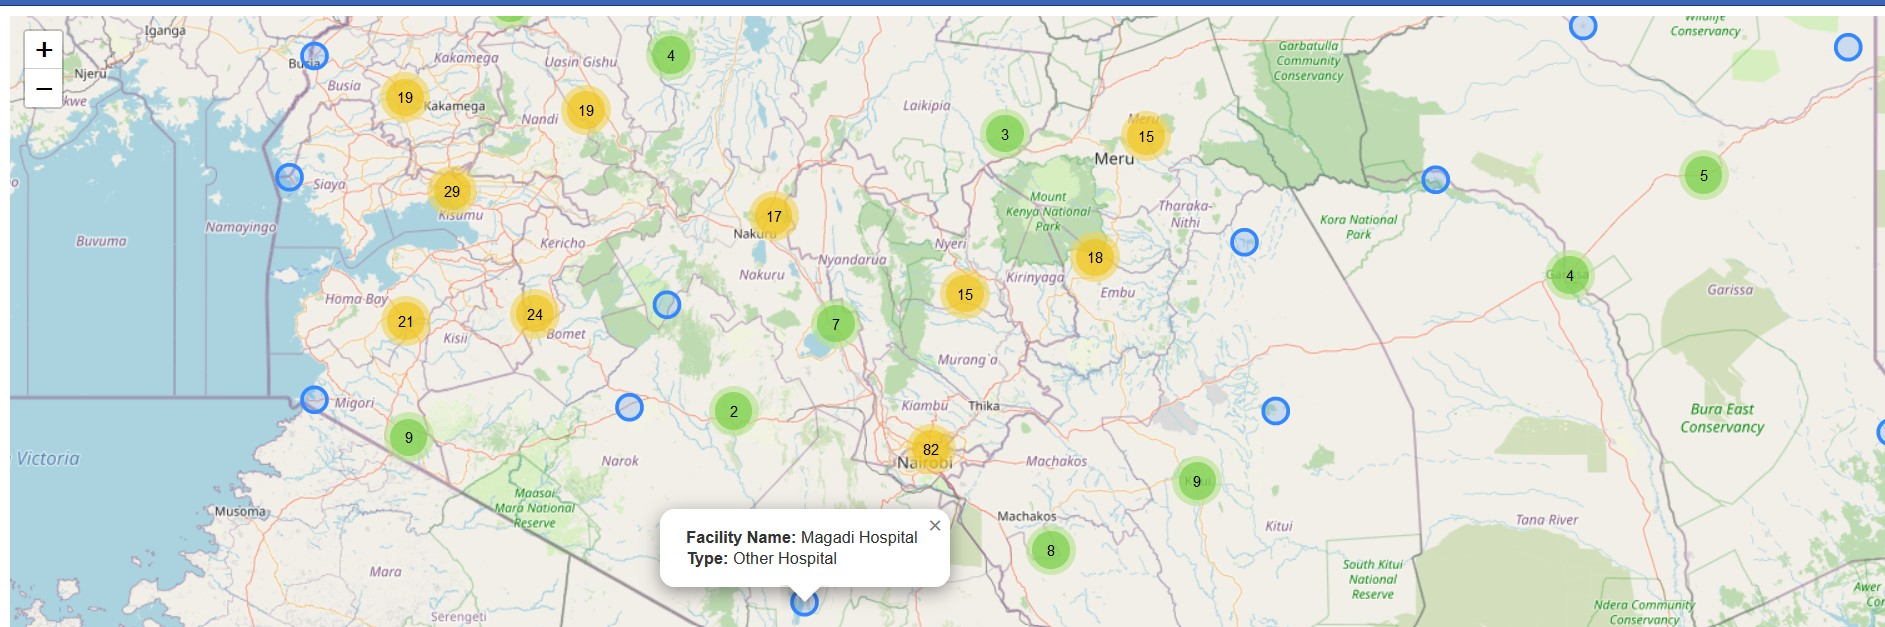
\includegraphics[width=26.18in]{../images/cluster-marker-map-fixed}

Now all points have their rightful and respective names.

\hypertarget{additional-features-of-cluster-marker-plugin}{%
\section{Additional features of Cluster marker plugin}\label{additional-features-of-cluster-marker-plugin}}

The official documentation of the plugin lists many other features that come along with the tool. We can't go through all of them, neither is there the will but let's summise just one important one: the \texttt{mouseover} event. The same way that leaflet's markers can have events triggered on them also applies to the Cluster marker plugin. Below is an example in their webpage

\begin{verbatim}
// We won't use this

markers.on('click', function (a) {
    console.log('marker ' + a.layer);
});
\end{verbatim}

Let's demonstrate adding a hover event to our cluster marker map, thanks to this \href{https://gnisitricks.de/2019/03/Adding-Click-and-Mouseover-Events-simultaneously-to-GeoJson-Markers-on-a-Leaflet-Map/}{answer}.

\begin{verbatim}
/////// Added `mouseover` event

fetch(url)
    .then((response) =>{
        return response.json()
    })
    .then((data) => {
        var markers = L.markerClusterGroup({chunkedLoading: true}); // Splits the add layers to small intervals to prevent page freezing

        var geojsonGroup = L.geoJSON(data, {
            onEachFeature : function(feature, layer){
                layer.bindPopup(`<b>Facility Name:</b> ${feature.properties.Facility_N} <br>
                <b>Type:</b> ${feature.properties.Type}`);
            },
            pointToLayer: function (feature, latlng) {
                return L.circleMarker(latlng).on('mouseover', function(){
                    this.bindPopup(`Nearest_Center: ${feature.properties.Nearest_To}`).openPopup(); // Add mouseover event
                });
            }
        });

        markers.addLayer(geojsonGroup);
        map.addLayer(markers);

    })
    .catch((error) => {
        console.log(`This is the error: ${error}`)
    })
\end{verbatim}

From the above code, we added the \texttt{mouseover} event to each marker point using the \texttt{on} method. This was thanks to \texttt{this} keyword which refers to the object in the current code chunk --\texttt{geojsonGroup}. We also sped the rendering of our Leaflet map by adding \texttt{chunkedLoading:\ true} parameter to \texttt{L.markerCluster()} function.

Hovering over each marker point will show an attribute of the centre in closest proximity from the \texttt{Nearest\_To} properties of the Json Layer.

\begin{Shaded}
\begin{Highlighting}[]
\NormalTok{knitr}\SpecialCharTok{::}\FunctionTok{include\_graphics}\NormalTok{(}\FunctionTok{rep}\NormalTok{(}\StringTok{\textquotesingle{}D:/gachuhi/my{-}leaflet/images/cluster{-}marker{-}mouseover.jpg\textquotesingle{}}\NormalTok{))}
\end{Highlighting}
\end{Shaded}

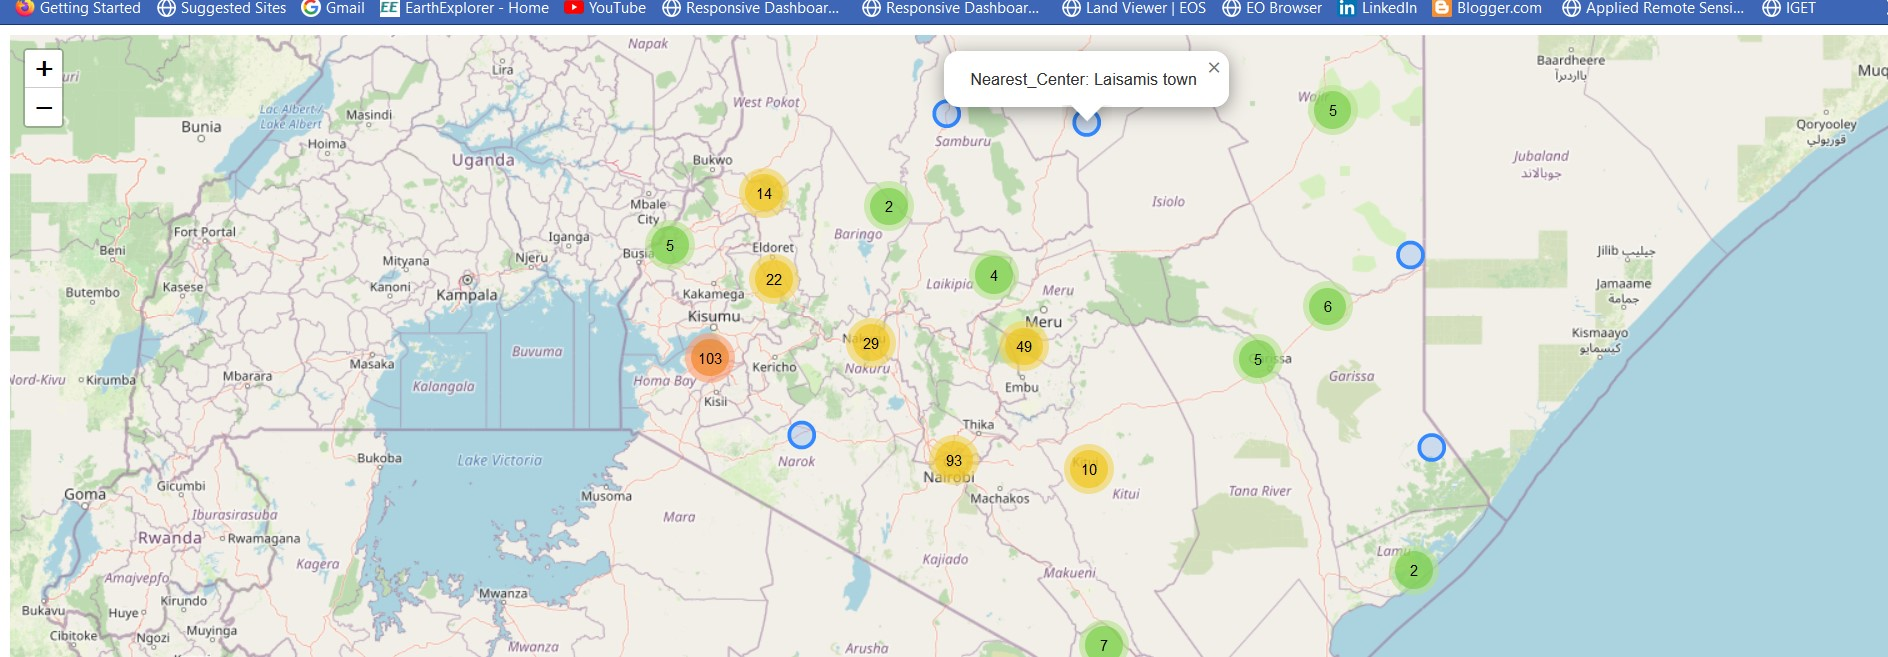
\includegraphics[width=26.22in]{../images/cluster-marker-mouseover}

The code files used for this chapter are available from \href{https://www.dropbox.com/scl/fo/vbyxk75jodchlgxb4obkl/h?dl=0\&rlkey=x5jya8iwtj431uwxte7usdvpa}{here}.

\hypertarget{mobile-friendly-webapps}{%
\chapter{Mobile Friendly Webapps}\label{mobile-friendly-webapps}}

Short story. Not too long ago I was the proud owner of a famous phone brand on the decline. The phone was like an extension of my personality for I understood its shortcomings, while on the other hand, it perfectly blended, nearing understanding what I wanted and needed, and providing exactly that.

One time, when taking a photo of the iconic Ngong Hills for Wikipedia's Africa Climate photo contest, the phone just died. That was it. A quick visit to the authorized dealer was greeted with the unbelievable and bemusing words of, ``We no longer ship the motherboard to the country anymore.'' Some healing has taken place, but I was totally heartbroken, and occasionaly suffer some nostalgia of the `good times' I had with my phone.

It's been a long ride with leaflet, you need a breather. Anyway, webapps can be heavy, and they can load slowly on smaller devices such as smartphones. Apps that load slow can put off your web app users, so it is prudent to customize your webapp for your user's phones.

``Well, what the heck?'', you may ask, ``It will just test their patience for a couple few second\ldots{}'' Alright, I get it. Why the hustle to make the app mobile friendly just to appease someone's impatience. If you think that your user's will only be using your webapp on a laptop, you are wrong. If they won't find it friendly on their smartphone they may not think twice on using it on a laptop either.

Let's get on with making our cluster marker app mobile friendly. We shall also add other functionalities to make the web app heavy, and thus test our mobile-friendly web map making to destruction.

\hypertarget{the-basemaps}{%
\section{The basemaps}\label{the-basemaps}}

If you have gone through the \protect\hyperlink{layer-groups-and-controls}{Chapter 8} of creating controls the following will look familiar. We will add some basemaps and later on create their control widgets.

\begin{verbatim}
// Basemaps
var osm = L.tileLayer('https://tile.openstreetmap.org/{z}/{x}/{y}.png', {
    maxZoom: 19,
    attribution: '&copy; <a href="http://www.openstreetmap.org/copyright">OpenStreetMap</a>'
});

var cyclOSM = L.tileLayer('https://{s}.tile-cyclosm.openstreetmap.fr/cyclosm/{z}/{x}/{y}.png', {
    maxZoom: 20,
    attribution: '<a href="https://github.com/cyclosm/cyclosm-cartocss-style/releases" title="CyclOSM - Open Bicycle render">CyclOSM</a> | Map data: &copy; <a href="https://www.openstreetmap.org/copyright">OpenStreetMap</a> contributors'
}); // the CyclOSM tile layer available from Leaflet servers
\end{verbatim}

Let's add our basemaps to Leaflet.

\begin{verbatim}
// Add the Leaflet basemaps
var map = L.map('myMap', {
    layers: [osm, cyclOSM]
}).setView([-1.295287148, 36.81984753], 7);
\end{verbatim}

\hypertarget{adding-the-features}{%
\section{Adding the features}\label{adding-the-features}}

Remember our hospital json layer. Let's call it again and transform it to a cluster marker with \texttt{fetch}.

\begin{verbatim}
// Add hospital dataset

url = 'https://raw.githubusercontent.com/sammigachuhi/geojson_files/main/selected_hospitals.json'

var cluster = fetch(url)
    .then((response) =>{
        return response.json()
    })
    .then((data) => {
        var markers = L.markerClusterGroup();

        var geojsonGroup = L.geoJSON(data, {
            onEachFeature : function(feature, layer){
                var popupContent =  `<b>Facility Name:</b> ${feature.properties.Facility_N} <br>
                <b>Type:</b> ${feature.properties.Type}`;
                layer.bindPopup(popupContent)
            },
            pointToLayer: function (feature, latlng) {
                return L.circleMarker(latlng);
            }
        });

        markers.addLayer(geojsonGroup);
        map.addLayer(markers);

    })
    .catch((error) => {
        console.log(`This is the error: ${error}`)
    })
\end{verbatim}

Why assing the \texttt{fetch} code to the variable \texttt{var\ cluster}. Well, we were aiming for the stars. We wanted to have a layer control for our \texttt{cluster} variable too but unfortunately this plan failed. You will see later on.

Let's put our \texttt{basemaps} and \texttt{cluster} variables into JavaScript objects to create a layer control for each.

\begin{verbatim}
// Set object for the basemaps
var basemaps = {
    "OpenStreetMap": osm,
    'cycleOsm': cyclOSM,
}

////Don't add the 'overlays' object. For demonstration purposes only
// Set object for the overlay maps
var overlays = {
    'Hospitals': cluster
}
\end{verbatim}

Before you head on any further, let me tell you the result of inserting the \texttt{overlays} object into the \texttt{L.control.Layers()} class. A liturgy of errors results.

\begin{Shaded}
\begin{Highlighting}[]
\NormalTok{knitr}\SpecialCharTok{::}\FunctionTok{include\_graphics}\NormalTok{(}\FunctionTok{rep}\NormalTok{(}\StringTok{\textquotesingle{}D:/gachuhi/my{-}leaflet/images/mobile{-}friendly{-}error.jpg\textquotesingle{}}\NormalTok{))}
\end{Highlighting}
\end{Shaded}

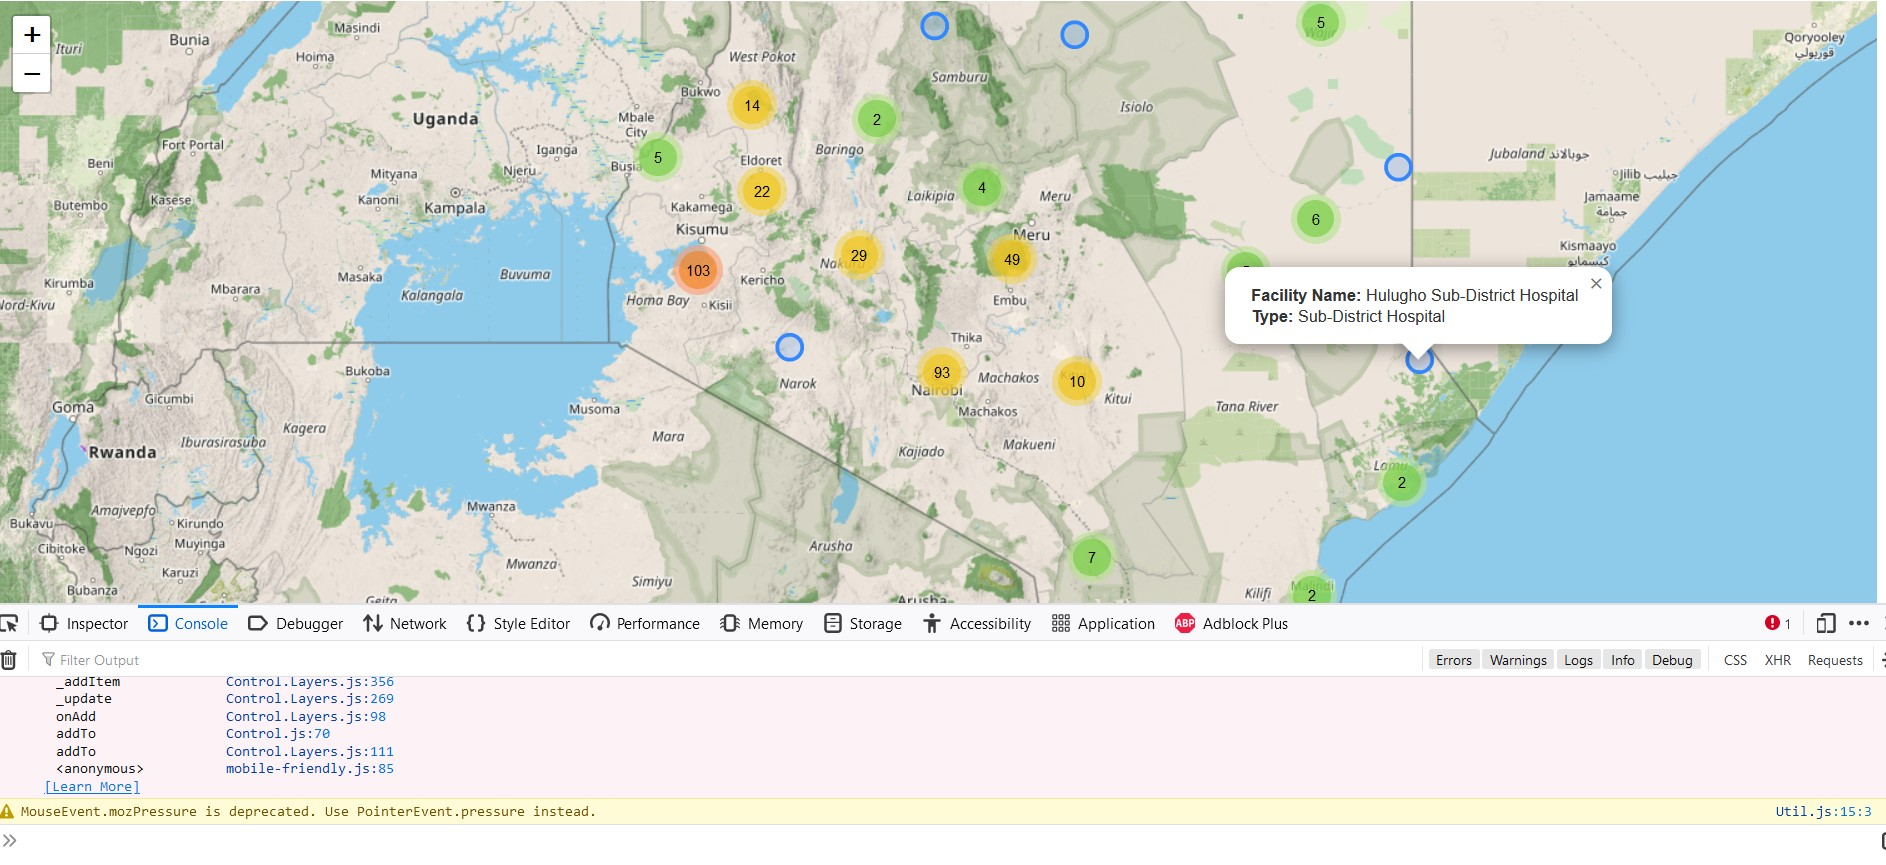
\includegraphics[width=26.19in]{../images/mobile-friendly-error}

The webmap works alright, showing popups and all, but there is a list of errors on our console. The one listed as \texttt{\textless{}anonymous\textgreater{}\ mobile-friendly.js:85} actually refers to our \texttt{L.control.Layers()} class, and it is without a doubt (no) thanks to the \texttt{overlays} argument. It's because \texttt{overlays} contains \texttt{fetch} which we suspect is behind all these problems. Removing the \texttt{overlays} argument and the object altogether eliminates this error.

Incase you had jumped headlong into the pit with me, comment out the \texttt{overlays} object and add \texttt{L.controLayers()}.

\hypertarget{zooming-to-mobile-users-location}{%
\section{Zooming to mobile user's location}\label{zooming-to-mobile-users-location}}

According to the Leaflet official documentation, Leaflet has a handy shortcut of zooming in to the user's location, if not a geofence of his exact position.

\begin{verbatim}
// Zoom to your location
map.locate({setView: true, maxZoom: 16});
\end{verbatim}

\hypertarget{add-marker-to-mobile-users-geolocation}{%
\section{Add marker to mobile user's geolocation}\label{add-marker-to-mobile-users-geolocation}}

Even if the location is off by a couple of miles, at least a marker to show the triangulated position will help. At least you will not be \emph{all over} the map! The following code adds a marker to the mobile user's triangulated Latitude-Longitude coordinates, and displays a message showing the radius in which the mobile user is most likely to be found from the marker point.

\begin{verbatim}
// Add marker at your location
function onLocationFound(e) {
    var radius = e.accuracy;

    L.marker(e.latlng).addTo(map)
        .bindPopup("You are within " + Number((radius/1000).toFixed(2)) + " kilometers from this point").openPopup();

    L.circle(e.latlng, radius).addTo(map);
}
\end{verbatim}

Incase you forgot, the \texttt{on} method adds listeners. As a gentle reminder, listeners are codes that run when an event, as simple as hovering or as intensive as double clicking are triggered. In the below code, the listener \texttt{\textquotesingle{}locationfound\textquotesingle{}} it triggers the \texttt{onLocationFound} function in case approximating the mobile user's location went successfully.

\begin{verbatim}
map.on('locationfound', onLocationFound);
\end{verbatim}

The \texttt{locationfound} listener is responsible for the message bounded in red when I first load my map. Clicking \textbf{Allow} will give the browser the heads up to zoom to my location as it best can.

\begin{Shaded}
\begin{Highlighting}[]
\NormalTok{knitr}\SpecialCharTok{::}\FunctionTok{include\_graphics}\NormalTok{(}\FunctionTok{rep}\NormalTok{(}\StringTok{\textquotesingle{}D:/gachuhi/my{-}leaflet/images/location{-}found.jpg\textquotesingle{}}\NormalTok{))}
\end{Highlighting}
\end{Shaded}

\includegraphics[width=26.49in]{../images/location-found}

What if, getting the mobile user's geolocation is unsuccessful? We will create a function that outputs the error event to our console, as shown below.

\begin{verbatim}
// Error displayed after finding location failed
function onLocationError(e) {
    alert(e.message);
}
\end{verbatim}

Actually, \texttt{message} is an error event that displays the error message of a parameter, in this case the layer. We finally add this \texttt{onLocationError} function to the map. It will be triggered if the \texttt{\textquotesingle{}locationerror\textquotesingle{}} event is true!

\begin{verbatim}
map.on('locationerror', onLocationError);
\end{verbatim}

\hypertarget{the-mobile-webmap-app-in-action}{%
\section{The mobile webmap app in action!}\label{the-mobile-webmap-app-in-action}}

Yours truly has save you the hustle of detailing how this chapter's files have been saved to Github, and converted into a webpage. However, I provide the link to view the web app on your phone. Chances are high it will not fail on you like mine did to me ;). Below is the link. Try it on your phone!

\url{https://sammigachuhi.github.io/hospitals_webapp/}

\begin{Shaded}
\begin{Highlighting}[]
\NormalTok{knitr}\SpecialCharTok{::}\FunctionTok{include\_graphics}\NormalTok{(}\FunctionTok{rep}\NormalTok{(}\StringTok{\textquotesingle{}D:/gachuhi/my{-}leaflet/images/mobile{-}app.jpg\textquotesingle{}}\NormalTok{))}
\end{Highlighting}
\end{Shaded}

\includegraphics[width=8in]{../images/mobile-app}

Remember me mentioning I was aiming for the stars by wanting to add the hospital markers as a layer control? Well, I landed on the skies since you can see that only the basemaps could be added to the layers control widget.

However, this looks like a good hospital locations app! The sky was only the baseline!

The full code script is available from \href{https://www.dropbox.com/scl/fo/lu6xoy9vcwrtruc838e29/h?dl=0\&rlkey=suuajpnxon0axc7y4r5s3yh0f}{here}.

\hypertarget{web-map-service-layers}{%
\chapter{Web Map Service Layers}\label{web-map-service-layers}}

\hypertarget{what-are-web-map-service-wms-layers}{%
\section{What are Web Map Service (WMS) Layers?}\label{what-are-web-map-service-wms-layers}}

A \href{https://gisgeography.com/web-mapping-services-wms/}{Web Mapping Service (WMS)} consists of geospatial data hosted through the internet with standards set by the Open Geospatial Consortium (OGS).

A WMS enables the exchange of spatial information and viewing over the web in the form of a map or image to your browser. The most common formats of WMS are WMS, WFS, WCS, WPS, WMTS, and WCPS. WMS is the most used. It offers basic panning, zooming and somewhat quick rendering speeds.

\hypertarget{loading-a-wms-server}{%
\section{Loading a WMS server}\label{loading-a-wms-server}}

To load a WMS layer into leaflet, we use the \texttt{L.tileLayer.wms} class. As simple as that. So let's set up our Leaflet map. Create a new JavaScript file named \texttt{wms\_layers.js} and insert the following code.

\begin{verbatim}
let map = L.map('myMap').setView([-1.295287148, 36.81984753], 7);

let tileLayer = L.tileLayer('https://tile.openstreetmap.org/{z}/{x}/{y}.png', {
    maxZoom: 19,
    attribution: '&copy; <a href="http://www.openstreetmap.org/copyright">OpenStreetMap</a>'
});
\end{verbatim}

We have added an OSM layer because we want to create a layer control widget that also contains WMS layers so that you can switch between both for either spatial awareness or informational purposes (WMS layer). Without further ado, let's add two WMS layers.

\begin{verbatim}
let wmsLayerTopo = L.tileLayer.wms('https://www.gmrt.org/services/mapserver/wms_merc_mask?', {
    layers: 'topo',
    format: 'image/png'
})

let wmsLayerTopomask = L.tileLayer.wms('https://www.gmrt.org/services/mapserver/wms_merc_mask?', {
    layers: 'topo-mask',
    format: 'image/png'
})
\end{verbatim}

\hypertarget{adding-wms-to-layer-control}{%
\section{Adding WMS to layer control}\label{adding-wms-to-layer-control}}

Let's insert the above web map layers into a JavaScript object before passing it to a layer control.

\begin{verbatim}
var basemaps = {
    OSM: tileLayer,
    Topo: wmsLayerTopo,
    Topo_mask: wmsLayerTopomask,
}
\end{verbatim}

Now let's parse the object into a control. If you did \protect\hyperlink{layer-groups-and-controls}{Chapter 8} then this should be familiar.

\begin{verbatim}
L.control.layers(basemaps).addTo(map);

basemaps.Topo.addTo(map);  // To have the Topo as the default map layer
\end{verbatim}

The last line \texttt{basemaps.Topo.addTo(map)} serves to set up the default layer that will appear when the map is loaded. In this case it is the variable set to \texttt{Topo} key in \texttt{var\ basemaps}. If this last line is omitted, the leaflet map will load alright, however, it will be blank canvas unless one of the radioitems is clicked.

\begin{Shaded}
\begin{Highlighting}[]
\NormalTok{knitr}\SpecialCharTok{::}\FunctionTok{include\_graphics}\NormalTok{(}\FunctionTok{rep}\NormalTok{(}\StringTok{\textquotesingle{}D:/gachuhi/my{-}leaflet/images/wms\_layer.jpg\textquotesingle{}}\NormalTok{))}
\end{Highlighting}
\end{Shaded}

\includegraphics[width=26.67in]{../images/wms_layer}

And that's it!

We wanted to introduce some African-based WMS layers, of which \href{https://training.digitalearthafrica.org/en/latest/OWS_tutorial.html}{Digital Earth Africa} provides a couple, however, these WMS layers could only be loaded in Qgis. Subsequent attempts to load them in Leaflet even after carefully following the official documents yielded no fruits.

Interested in getting other WMS layers? Go to \href{https://directory.spatineo.com/}{Spartineo.com}.

The files used in these very short chapter are available \href{https://www.dropbox.com/scl/fo/n6oiyw21axiqxpdcfeqnp/h?dl=0\&rlkey=jr8f6g5mx5i83kpjofv56hk5g}{here}.

\hypertarget{standard-website-with-leaflet-project}{%
\chapter{Standard Website with Leaflet Project}\label{standard-website-with-leaflet-project}}

\hypertarget{get-the-html-template}{%
\section{Get the HTML Template}\label{get-the-html-template}}

Remember me trying to insert a leaflet map into some lousy looking website to do with GMOs back in \protect\hyperlink{embedding-leaflet-map-to-an-external-website}{Chapter 4}? Well, there is a aphomism in my local lingo that says only the stay at home thinks that their household cooks well. It is until you challenge yourself with something new that you can prove your salt. In this chapter, we would like to demonstrate how leaflet can be added to a standard HTML website. The purpose of this chapter is to train you how you can insert a leaflet map to your company's, client's or even colleague's website if called upon. They heard you are a web mapping master. So why not?

The template used in this exercise was acquired from Free CSS.com and is available \href{https://www.free-css.com/assets/files/free-css-templates/download/page291/elearning.zip}{here}. Extract the files and take a look at the html documents. That is, the \texttt{index.html}, \texttt{about.html}, \texttt{contact.html}, \texttt{courses.html}, \texttt{team.html} and \texttt{testimonial.html}. Pay special attention to the \texttt{\textless{}head\textgreater{}} element and the \texttt{\textless{}div\textgreater{}} containing the Gallery section of the website. The Gallery \texttt{\textless{}div\textgreater{}} looks like so:

\begin{verbatim}
<div class="col-lg-3 col-md-6">
                    <h4 class="text-white mb-3">Gallery</h4>
                    <div class="row g-2 pt-2">
                        <div class="col-4">
                            <img class="img-fluid bg-light p-1" src="img/course-1.jpg" alt="">
                        </div>
                        <div class="col-4">
                            <img class="img-fluid bg-light p-1" src="img/course-2.jpg" alt="">
                        </div>
                        <div class="col-4">
                            <img class="img-fluid bg-light p-1" src="img/course-3.jpg" alt="">
                        </div>
                        <div class="col-4">
                            <img class="img-fluid bg-light p-1" src="img/course-2.jpg" alt="">
                        </div>
                        <div class="col-4">
                            <img class="img-fluid bg-light p-1" src="img/course-3.jpg" alt="">
                        </div>
                        <div class="col-4">
                            <img class="img-fluid bg-light p-1" src="img/course-1.jpg" alt="">
                        </div>
                    </div>
                </div>
\end{verbatim}

Here is where the Gallery in the elearning webpage is situated.

\begin{Shaded}
\begin{Highlighting}[]
\NormalTok{knitr}\SpecialCharTok{::}\FunctionTok{include\_graphics}\NormalTok{(}\FunctionTok{rep}\NormalTok{(}\StringTok{\textquotesingle{}D:/gachuhi/my{-}leaflet/images/gallery.jpg\textquotesingle{}}\NormalTok{))}
\end{Highlighting}
\end{Shaded}

\includegraphics[width=26.14in]{../images/gallery}

Why do we want to change the gallery, or rather, to insert a leaflet map in its place? Well, I decided to be mean on it. Sorry, that wasn't supposed to come out of my mouth. Candidly speaking, the Gallery section only contained some pretty pictures and personally I felt replacing them with a leaflet map would serve as the best demonstration for this chapter.

\hypertarget{insert-leaflet-to-standard-html-website}{%
\section{Insert Leaflet to standard html website}\label{insert-leaflet-to-standard-html-website}}

Since we want to insert a leaflet to the eLearning website, we will have to load the requisite Leaflet links and scripts to the websites \texttt{\textless{}head\textgreater{}} element, just like we used to do to our \texttt{map.html}. Thereafter, we shall replace the entire gallery section with just one \texttt{\textless{}div\textgreater{}} that references one of our many Leaflet JavaScript files.

Ready? Let's go.

Assuming you are working on VSCode, copy all the plugin files for leaflet, such as \texttt{Leaflet.markercluster-master} folder and others you had extracted prior to parsing them to your javascript files. Perhaps an image will make the instructions clearer. The below files should be in your eLearning template folder.

\begin{Shaded}
\begin{Highlighting}[]
\NormalTok{knitr}\SpecialCharTok{::}\FunctionTok{include\_graphics}\NormalTok{(}\FunctionTok{rep}\NormalTok{(}\StringTok{\textquotesingle{}D:/gachuhi/my{-}leaflet/images/elearning{-}plugins.jpg\textquotesingle{}}\NormalTok{))}
\end{Highlighting}
\end{Shaded}

\includegraphics[width=13.69in]{../images/elearning-plugins}

Why are we ensuring that the leaflet plugin folders are in the same directory of our eLearning template files? YOu will know in a tid bit.

Go to the \texttt{index.html} file of your eLearning template. From the \texttt{\textless{}head\textgreater{}} to \texttt{\textless{}/head\textgreater{}} tags, replace the existing code with the following:

\begin{verbatim}
<meta charset="utf-8">
    <!-- For leaflet and mobile compatibility -->
    <meta name="viewport" content="width=device-width, initial-scale=1.0, maximum-scale=1.0, user-scalable=no" />

    <title>eLEARNING - eLearning HTML Template</title>
    <meta content="width=device-width, initial-scale=1.0" name="viewport">
    <meta content="" name="keywords">
    <meta content="" name="description">

    <!-- Favicon -->
    <link href="img/favicon.ico" rel="icon">

    <!-- Google Web Fonts -->
    <link rel="preconnect" href="https://fonts.googleapis.com">
    <link rel="preconnect" href="https://fonts.gstatic.com" crossorigin>
    <link href="https://fonts.googleapis.com/css2?family=Heebo:wght@400;500;600&family=Nunito:wght@600;700;800&display=swap" rel="stylesheet">

    <!-- Icon Font Stylesheet -->
    <link href="https://cdnjs.cloudflare.com/ajax/libs/font-awesome/5.10.0/css/all.min.css" rel="stylesheet">
    <link href="https://cdn.jsdelivr.net/npm/bootstrap-icons@1.4.1/font/bootstrap-icons.css" rel="stylesheet">

    <!-- Libraries Stylesheet -->
    <link href="lib/animate/animate.min.css" rel="stylesheet">
    <link href="lib/owlcarousel/assets/owl.carousel.min.css" rel="stylesheet">

    <!-- Customized Bootstrap Stylesheet -->
    <link href="css/bootstrap.min.css" rel="stylesheet">

    <!-- Template Stylesheet -->
    <link href="css/style.css" rel="stylesheet">

    <!-- For leaflet -->
    <link rel="stylesheet" href="https://unpkg.com/leaflet@1.9.3/dist/leaflet.css"
        integrity="sha256-kLaT2GOSpHechhsozzB+flnD+zUyjE2LlfWPgU04xyI="
        crossorigin=""/>
    <link rel="stylesheet" href="Leaflet.Control.Opacity-master\Leaflet.Control.Opacity-master\dist\L.Control.Opacity.css">
    <!-- For Leaflet marker clusters -->
    <link rel="stylesheet" href="Leaflet.markercluster-master\Leaflet.markercluster-master\dist\MarkerCluster.Default.css">  

    <!-- For leaflet scripts -->
    <script src="https://unpkg.com/leaflet@1.9.3/dist/leaflet.js"
        integrity="sha256-WBkoXOwTeyKclOHuWtc+i2uENFpDZ9YPdf5Hf+D7ewM="
        crossorigin=""></script>
    <script src="leaflet-ajax-gh-pages\dist\leaflet.ajax.js"></script>
    <script src="leaflet-ajax-gh-pages\dist\leaflet.ajax.min.js"></script>
    <script src="leaflet-ajax-gh-pages\example\leaflet.spin.js"></script>
    <script src="leaflet-ajax-gh-pages\example\spin.js"></script> 
    <script src="Leaflet.heat-gh-pages\Leaflet.heat-gh-pages\dist\leaflet-heat.js"></script>
    <script src="https://ajax.googleapis.com/ajax/libs/jquery/2.1.4/jquery.min.js"></script>
    <!-- For leaflet cluster markers -->
    <script src="Leaflet.markercluster-1.4.1\Leaflet.markercluster-1.4.1\dist\leaflet.markercluster.js"></script>
    <script src="Leaflet.markercluster-1.4.1\Leaflet.markercluster-1.4.1\dist\leaflet.markercluster-src.js"></script>
    
\end{verbatim}

We have just retained the existing code and added the leaflet \texttt{\textless{}link\textgreater{}} and \texttt{\textless{}script\textgreater{}} tags we have experienced so far -- from good old \texttt{map.html} of course. Before I forget, here's why the leaflet plugin folders have to be together with the eLearning files. When we copied our \texttt{\textless{}link\textgreater{}} and \texttt{\textless{}script\textgreater{}} tags from \texttt{map.html} they were referring to certain paths. When you paste them to the \texttt{index.html} of your eLearning template, the path's are no longer correct. They have just been placed in a destination/directory! However, if you paste the Leaflet folders you have worked with so far so that they are within the same directory, you don't have to (painfully) change the paths because they will remain \emph{correct}.

Didn't get me? Take the following \texttt{\textless{}script\textgreater{}} tag.

\begin{verbatim}
<script src="Leaflet.markercluster-1.4.1\Leaflet.markercluster-1.4.1\dist\leaflet.markercluster.js"></script>
\end{verbatim}

It still remains correct within the \texttt{index.html} of our eLearning template because we have pasted the same \texttt{Leaflet.markercluster-1.4.1} folder in the same directory as other eLearning template file. ie. the path still refers to the same place. No adventuring to other folder inside or outside the same eLearning template directory!

Another small favour. Copy and past the \texttt{cluster\_markers.js} file into the eLearning template directory.

Alright.

A glass of water.

Back to the screen.

Time to add the leaflet map. Where? At the gallery section.

As a reminder, it looks like this:

\begin{verbatim}
<div class="col-lg-3 col-md-6">
                    <h4 class="text-white mb-3">Gallery</h4>
                    <div class="row g-2 pt-2">
                        <div class="col-4">
                            <img class="img-fluid bg-light p-1" src="img/course-1.jpg" alt="">
                        </div>
                        <div class="col-4">
                            <img class="img-fluid bg-light p-1" src="img/course-2.jpg" alt="">
                        </div>
                        <div class="col-4">
                            <img class="img-fluid bg-light p-1" src="img/course-3.jpg" alt="">
                        </div>
                        <div class="col-4">
                            <img class="img-fluid bg-light p-1" src="img/course-2.jpg" alt="">
                        </div>
                        <div class="col-4">
                            <img class="img-fluid bg-light p-1" src="img/course-3.jpg" alt="">
                        </div>
                        <div class="col-4">
                            <img class="img-fluid bg-light p-1" src="img/course-1.jpg" alt="">
                        </div>
                    </div>
                </div>
\end{verbatim}

You may have to scroll \emph{really} down to locate it. Right under the \texttt{\textless{}h4\ class="text-white\ mb-3"\textgreater{}Gallery\textless{}/h4\textgreater{}} tag, replace it with the following code, all the to the \texttt{\textless{}div\textgreater{}} tag after \texttt{\textless{}img\ class="img-fluid\ bg-light\ p-1"\ src="img/course-1.jpg"\ alt=""\textgreater{}}.

\begin{verbatim}
<div id="myMap"> 
                        <script src="cluster-markers.js">

                        </script>
                    </div>
\end{verbatim}

Perhaps an image will clarify matters a bit. This is how it should look:

\begin{Shaded}
\begin{Highlighting}[]
\NormalTok{knitr}\SpecialCharTok{::}\FunctionTok{include\_graphics}\NormalTok{(}\FunctionTok{rep}\NormalTok{(}\StringTok{\textquotesingle{}D:/gachuhi/my{-}leaflet/images/div\_replace.jpg\textquotesingle{}}\NormalTok{))}
\end{Highlighting}
\end{Shaded}

\includegraphics[width=20.99in]{../images/div_replace}

Also as a heads up, remember to replace the \texttt{\textless{}h4\textgreater{}} tags with the statement \texttt{Our\ Location}. It's no longer a gallery!

As if that was not enough, going easy on our fingers and all, we have to set the CSS properties for our leaflet map.

\hypertarget{editing-the-css}{%
\section{Editing the CSS}\label{editing-the-css}}

Open the \texttt{style.css} file of your eLearning template in your text editor (such as VS code). The path to the CSS file is as follows:

\begin{verbatim}
elearning-template\css\style.css
\end{verbatim}

Scroll down to the very bottom of \texttt{style.css} and paste the following CSS properites for our Leaflet map.

\begin{verbatim}
#myMap { 
    height: 400px;
    width: auto; 
}
\end{verbatim}

Remember the \texttt{\#} and the text that follows references the specifically named \texttt{id} attribute in the tags of our html element. In the above case, it references the \texttt{\textless{}div\textgreater{}} with the ID \texttt{\#myMap}.

After reloading \texttt{index.html}, this is how our leaflet map looks inside the eLearning template.

\begin{Shaded}
\begin{Highlighting}[]
\NormalTok{knitr}\SpecialCharTok{::}\FunctionTok{include\_graphics}\NormalTok{(}\FunctionTok{rep}\NormalTok{(}\StringTok{\textquotesingle{}D:/gachuhi/my{-}leaflet/images/location\_elearning.jpg\textquotesingle{}}\NormalTok{))}
\end{Highlighting}
\end{Shaded}

\includegraphics[width=26.28in]{../images/location_elearning}

Good.

\hypertarget{adding-leaflet-to-every-webpage}{%
\section{Adding leaflet to every webpage}\label{adding-leaflet-to-every-webpage}}

Now click the \textbf{About}, \textbf{Courses}, \textbf{Pages/Our Team}, \textbf{Pages/Testimonial} and \textbf{Contact} web pages. Is the leaflet map there? No.~It's the gallery. Imagine you will have to replace the \texttt{\textless{}head\textgreater{}} and Gallery \texttt{\textless{}div\textgreater{}} elements here as well!

``How and I don't have the time?!!'' If you look at the eLearning template directory, you will see the \textbf{about}, \textbf{courses}, \textbf{contact}, \textbf{team} and \textbf{testimonial} html files. Replace their \texttt{\textless{}head\textgreater{}} elements and Gallery \texttt{\textless{}div\textgreater{}}s just as you did for \texttt{index.html}. Luckily I am your hero. This was done for you and the files are available \href{https://github.com/sammigachuhi/elearning_template_demo.git}{here}.

\hypertarget{posting-the-html-website-to-the-world}{%
\section{Posting the Html website to the world}\label{posting-the-html-website-to-the-world}}

This chapter will leave out the details of saving your files to Github. However, here's a clue. In order to automatically render a file in Github online, make sure the root html file is named \texttt{index.html}. These are taken as the default root html files by Github.

Yours truly already saved the file to Github. Here's the link to the file \href{https://sammigachuhi.github.io/elearning_template_demo/}{live and online}.

\hypertarget{leaflet-in-esri}{%
\chapter{Leaflet in ESRI}\label{leaflet-in-esri}}

Alright. If you are a GIS practitioner, you have (most) probably heard about ESRI, one of the world's leading geospatial software and services provider. You (might) have also come across various ESRI basemap servers, such as topographic, streets and imagery layers. They also have plugins that allow leaflet users to access the ArcGIS functionalities. For example, the ESRI plugins for leaflet allow you to access some ESRI basemaps and products, while also allowing you to become an ESRI ArcGIS JavaScript developer. Quite a mouthful of a career name.

To use ESRI Leaflet, you have to create an \href{https://developers.arcgis.com/dashboard/}{ArcGIS Developer account} and also get an \href{https://developers.arcgis.com/esri-leaflet/authentication/create-an-api-key/}{API key}. Kindly do so before proceeding.

\hypertarget{esri-leaflet-plugins}{%
\section{ESRI Leaflet plugins}\label{esri-leaflet-plugins}}

As we had mentioned earlier, you need ESRI leaflet plugins to fire up ESRI power in your leaflet environment. Alright. Remember your \texttt{map.html} file? You have probably added a plethora of \texttt{\textless{}link\textgreater{}}s and \texttt{\textless{}script\textgreater{}}s to your \texttt{map.html} file but bear with us a little longer. Add the following \texttt{\textless{}script\textgreater{}}s to the \texttt{\textless{}head\textgreater{}} element of your \texttt{map.html}.

\begin{verbatim}
<!-- Load Esri Leaflet from CDN -->
        <script src="https://unpkg.com/esri-leaflet@3.0.10/dist/esri-leaflet.js"></script>
        <script src="https://unpkg.com/esri-leaflet-vector@4.0.2/dist/esri-leaflet-vector.js"></script>
\end{verbatim}

Create a new JavaScript file called \texttt{esri\_leaflet.js} and get ready to enjoy ESRI services as though you made them!

\hypertarget{creating-an-esri-leaflet-map}{%
\section{Creating an ESRI Leaflet map}\label{creating-an-esri-leaflet-map}}

On your blank \texttt{esri\_leaflet.js} file, create a variable to store your Application Programming Interface (API) Key. This key is important to access your ESRI benefits, much like the magic phrase ``Open Sesame'' opens the doorway to a cave full of treasures as in the legendary story of \emph{Ali Baba and the Forty Thieves}. Of course I am no thief.

Below is an example of how to access your API key from your ArcGIS Developer account.

\begin{Shaded}
\begin{Highlighting}[]
\NormalTok{knitr}\SpecialCharTok{::}\FunctionTok{include\_graphics}\NormalTok{(}\FunctionTok{rep}\NormalTok{(}\StringTok{\textquotesingle{}D:/gachuhi/my{-}leaflet/images/esri\_leaflet\_api.jpg\textquotesingle{}}\NormalTok{))}
\end{Highlighting}
\end{Shaded}

\includegraphics[width=26.22in]{../images/esri_leaflet_api}

Copy paste that key to your \texttt{esri\_leaflet.js} file.

\begin{verbatim}
const apiKey = "Your key";
\end{verbatim}

Of course, don't expect me to showcase mine to the entire world.

Anyways, let's proceed to create a basemap. To create one, just create a variable called \texttt{basemapEnum} that stores the ESRI basemap identifier. What is that last thing? It is basically a basestyle map and in ESRI, at least when using Leaflet, it is accessed by parsing the provider name and the desired style, like so: \texttt{\{Provider\}:\{Style\ name\}} or
\texttt{\{Provider\}:\{Style\ name\}:\{Component\}}.

\begin{verbatim}
const basemapEnum = "ArcGIS:Streets";
\end{verbatim}

Alright. It's about time we fired up our mapping power. Create an ESRI leaflet map instance much like we have always been doing.

\begin{verbatim}
const map = L.map("myMap", {
    minZoom: 2
}).setView([0.3556, 37.5833], 6.5);
\end{verbatim}

We had created a basemap variable earlier, so we will parse it to the \texttt{L.esri.Vector.vectorBasemapLayer} class which is responsible for create basemaps. Actually one can also parse the \texttt{\{Provider\}:\{Style\ name\}} to the \texttt{L.esri.vector.vectorBasemapLayer()} class but our method of using variable names seems far much more cleaner.

\begin{verbatim}
L.esri.Vector.vectorBasemapLayer(basemapEnum, {
    apiKey: apiKey,
}).addTo(map);
\end{verbatim}

Now open your \texttt{map.html} file. What do you see?

\begin{Shaded}
\begin{Highlighting}[]
\NormalTok{knitr}\SpecialCharTok{::}\FunctionTok{include\_graphics}\NormalTok{(}\FunctionTok{rep}\NormalTok{(}\StringTok{\textquotesingle{}D:/gachuhi/my{-}leaflet/images/esri\_leaflet\_basemap.jpg\textquotesingle{}}\NormalTok{))}
\end{Highlighting}
\end{Shaded}

\includegraphics[width=26.57in]{../images/esri_leaflet_basemap}

Now imagine there are other styles as shown in this \href{https://developers.arcgis.com/documentation/mapping-apis-and-services/maps/services/basemap-layer-service/\#default-basemap-styles}{webpage}. Spoil yourself a bit.

\hypertarget{geocode-search}{%
\section{Geocode search}\label{geocode-search}}

Of course there are other ESRI Leaflet functionalities. I must confess I wanted to know how to add a raster layer, such as \texttt{.tif} to either Leaflet or ESRI leaflet but they all seem to favour tiled layers. The \href{https://github.com/GeoTIFF/georaster-layer-for-leaflet}{former has a plugin} to do so, but was too complicated (still trying unsuccessfully). Nevertheless, there are other cool services that ESRI leaflet offers, such as geocode search\footnote{Geocoding is the process of converting address or place text into a location. The geocoding service provides address and place geocoding as well as reverse geocoding}.

Let's do that.

\hypertarget{add-search-bar}{%
\section{Add search bar}\label{add-search-bar}}

Add the following \texttt{\textless{}link\textgreater{}} and \texttt{\textless{}script\textgreater{}} to your \texttt{\textless{}head\textgreater{}} element.

\begin{verbatim}
<!-- Load Esri Leaflet Geocoder from CDN -->
        <link rel="stylesheet" href="https://unpkg.com/esri-leaflet-geocoder@3.1.4/dist/esri-leaflet-geocoder.css">
        <script src="https://unpkg.com/esri-leaflet-geocoder@3.1.4/dist/esri-leaflet-geocoder.js"></script>
\end{verbatim}

Time to add a search control widget to the topright of our ESRI leaflet map. Search control widgets are created using the \texttt{L.esri.Geocoding.geosearch} class which we shall parse to a variable called \texttt{searchControl}.

\begin{verbatim}
const searchControl = L.esri.Geocoding.geosearch({
        position: "topright",
        placeholder: "Enter an address or place e.g. 1 York St",
        useMapBounds: false,

      }).addTo(map);
\end{verbatim}

Just like in leaflet ESRI leaflet constructors have their options. Please refer the options for this specific constructor \href{https://developers.arcgis.com/esri-leaflet/api-reference/controls/geosearch/}{here}.

Another small thing; change your \texttt{const\ basemapEnum} to read \texttt{ArcGis:Navigation}.

\begin{verbatim}
const basemapEnum = "ArcGIS:Navigation";
\end{verbatim}

If you refresh your \texttt{map.html} file, apart from having a new basemap style, you will see a new search bar at the top right. However, it is non-functional. It takes us nowhere.

\begin{Shaded}
\begin{Highlighting}[]
\NormalTok{knitr}\SpecialCharTok{::}\FunctionTok{include\_graphics}\NormalTok{(}\FunctionTok{rep}\NormalTok{(}\StringTok{\textquotesingle{}D:/gachuhi/my{-}leaflet/images/search\_bar.jpg\textquotesingle{}}\NormalTok{))}
\end{Highlighting}
\end{Shaded}

\includegraphics[width=26.19in]{../images/search_bar}

\hypertarget{make-the-search-bar-functional}{%
\section{Make the search bar functional}\label{make-the-search-bar-functional}}

In order to make the search bar do what it says, we will set the value of the \texttt{providers} key to a \texttt{arcgisOnlineProvider}. The latter is instantiated with the constructor \texttt{L.esri.Geocoding.arcgisOnlineProvider}. Okay where did you get it from? Well ESRI has various open source tutorials on its \href{https://developers.arcgis.com/esri-leaflet/geocode-and-search/search-for-an-address/?utm_source=pocket_saves}{platform}.

\begin{verbatim}
const searchControl = L.esri.Geocoding.geosearch({
    position: "topright",
    placeholder: "Enter an address or place e.g. 1 York St",
    useMapBounds: false,

    // Add provider
    providers: [
        L.esri.Geocoding.arcgisOnlineProvider({
          apikey: apiKey,
          nearby: {
            lat: 0.3556,
            lng: 37.5833
          }
        })
      ]

  }).addTo(map);
  
\end{verbatim}

Now try your search bar again. Some location names appear as you type them in, and if you press \textbf{Enter} it takes you to the exact location but there is no marker to pinpoint that specific address. We will sort that latter.

\begin{Shaded}
\begin{Highlighting}[]
\NormalTok{knitr}\SpecialCharTok{::}\FunctionTok{include\_graphics}\NormalTok{(}\FunctionTok{rep}\NormalTok{(}\StringTok{\textquotesingle{}D:/gachuhi/my{-}leaflet/images/searchable.jpg\textquotesingle{}}\NormalTok{))}
\end{Highlighting}
\end{Shaded}

\includegraphics[width=25.9in]{../images/searchable}

We will add a layer group to store the geocoding results.

\begin{verbatim}
const results = L.layerGroup().addTo(map);
\end{verbatim}

We will create an event handler to access the \texttt{data} from the search results. We shall also add a \texttt{clearLayers} call to remove the previous data from the layer group. This is beginning to sound complicated, but I'm just following along the \href{https://developers.arcgis.com/esri-leaflet/geocode-and-search/search-for-an-address/?utm_source=pocket_saves}{ESRI Leaflet geocoding tutorial}.

\begin{verbatim}
searchControl.on("results", (data) => {
        results.clearLayers();

      });
      
\end{verbatim}

The following loop adds the coordinates of the searched location to the marker. This loop goes into the \texttt{searchControl}.

\begin{verbatim}
for (let i = data.results.length - 1; i >= 0; i--) {
          const marker = L.marker(data.results[i].latlng);

          results.addLayer(marker);

        }
\end{verbatim}

The \texttt{lngLatString} variable below will store the rounded coordinates, and our familiar \texttt{bindPopup} and \texttt{openPopup} will show the coordinates and our address.

\begin{verbatim}
const lngLatString = `${Math.round(data.results[i].latlng.lng * 100000) / 100000}, ${
            Math.round(data.results[i].latlng.lat * 100000) / 100000
          }`;
          marker.bindPopup(`<b>${lngLatString}</b><p>${data.results[i].properties.LongLabel}</p>`);

          results.addLayer(marker);

          marker.openPopup();
\end{verbatim}

The entire \texttt{searchControl} code block should look like below.

\begin{verbatim}
searchControl.on("results", (data) => {
    results.clearLayers();

    for (let i = data.results.length - 1; i >= 0; i--) {
        const marker = L.marker(data.results[i].latlng);

        const lngLatString = `${Math.round(data.results[i].latlng.lng * 100000) / 100000}, ${
            Math.round(data.results[i].latlng.lat * 100000) / 100000
          }`;
          marker.bindPopup(`<b>${lngLatString}</b><p>${data.results[i].properties.LongLabel}</p>`);

        results.addLayer(marker);

        marker.openPopup();

      }

  });
  
\end{verbatim}

So now when you search for a particular place in the search bar and press \textbf{Enter}, a marker and with a pop up showcasing the address and longitude-latitude coordinates of the location should appear.

\begin{Shaded}
\begin{Highlighting}[]
\NormalTok{knitr}\SpecialCharTok{::}\FunctionTok{include\_graphics}\NormalTok{(}\FunctionTok{rep}\NormalTok{(}\StringTok{\textquotesingle{}D:/gachuhi/my{-}leaflet/images/search\_success.jpg\textquotesingle{}}\NormalTok{))}
\end{Highlighting}
\end{Shaded}

\includegraphics[width=26.15in]{../images/search_success}

There are many more tutorials on using ESRI Leaflet in the ArcGIS Developers website.

Here are the \href{https://www.dropbox.com/scl/fo/v5mqzkvpzz8um39c1810g/h?dl=0\&rlkey=2aptw30lln6s3hqxlay9al0y9}{files} used in this exercise.

\hypertarget{conclusion}{%
\chapter{Conclusion}\label{conclusion}}

Now here comes the end of our book. If you have reached this far, then congratulations! You now have the power to continue using leaflet to create cool webmaps, even far better than those you've encountered in this book.

I hope this book has been helpful. For anything that you found difficult to understand, or was without sufficient clarity, it had nothing to do with you.
\emph{Finis!}

  \bibliography{book.bib,packages.bib}

\end{document}
